% Main Thesis File - HKUST-GZ PhD Thesis
% Template: ustthesis.cls
\documentclass[a4paper]{ustthesis}

% ============================================================
% ESSENTIAL PACKAGES (required for compilation)
% ============================================================

% XeLaTeX font support (required for Chinese/fonts)
\usepackage{fontspec}
\setmainfont{Times New Roman}

% Mathematics
\usepackage{amsmath}
\usepackage{amssymb}
\usepackage{bm}              % Bold math symbols

% Tables and figures
\usepackage{booktabs}       % Publication-quality tables
\usepackage{array}
\usepackage{multirow}
\usepackage{tabularx}       % Variable-width table columns (required by Chapter 3)
\usepackage{graphicx}
\usepackage{rotating}       % Readable landscape placement for exceptionally wide figures
\usepackage{placeins}       % Keep floats within their semantic discussion blocks
\usepackage[table]{xcolor}

% Load subfig last to override template's subfigure and provide \subfloat
\usepackage[caption=false]{subfig}

% Algorithm and code (required by appendices)
\usepackage[ruled,vlined,linesnumbered]{algorithm2e}
\SetKwProg{Fn}{Function}{}{end}
\SetKwFunction{CHIPANNS}{C-HiPANNS}
\SetKwFunction{QHIPANNS}{Q-HiPANNS}

\usepackage{listings}
\lstdefinestyle{promptstyle}{
    basicstyle=\ttfamily\fontsize{9}{10.5}\selectfont,
    breaklines=true,
    backgroundcolor=\color{prompt-bg},
    frame=none,
    numbers=none,
    columns=fullflexible,
    keepspaces=true,
    showspaces=false,
    showstringspaces=false,
    tabsize=2,
    escapeinside=||,
    lineskip=-0.25pt
}

\usepackage[most]{tcolorbox}
\definecolor{prompt-bg}{RGB}{249,250,252}
\definecolor{prompt-border}{RGB}{96,110,135}

\newtcolorbox{promptbox}[1]{
    enhanced,
    breakable,
    arc=1.5pt,
    boxrule=0.45pt,
    colframe=prompt-border,
    colback=prompt-bg,
    title={\strut #1},
    titlerule=0pt,
    fonttitle=\bfseries\footnotesize,
    toptitle=1.5pt,
    bottomtitle=1pt,
    top=2pt,
    bottom=2pt,
    left=5pt,
    right=4pt,
    boxsep=0pt,
    colbacktitle=prompt-border
}

% Bibliography and links
% NOTE: hyperref should be loaded last (except for packages that must come after it)
\usepackage[numbers,sort&compress]{natbib}
\usepackage[colorlinks=true,linkcolor=black,citecolor=black,urlcolor=black]{hyperref}

\usepackage{xspace}
\usepackage{etoolbox}

% Preserve the indentation requested by the legacy class for each TOC level.
% Its TOC macro cancels the full left skip and relies on paragraph indentation,
% which is not retained here by current LaTeX. Cancel only the number width.
\makeatletter
\patchcmd{\@undottedtocline}
  {\parindent #2\relax\@afterindenttrue}
  {\parindent \z@\@afterindenttrue}
  {}
  {\PackageError{main}{Failed to patch table-of-contents indentation}{}}
\patchcmd{\@undottedtocline}
  {\@tempdima #3\relax \advance\leftskip \@tempdima \hbox{} \hskip -\leftskip}
  {\@tempdima #3\relax \advance\leftskip \@tempdima \null\nobreak\hskip -\@tempdima}
  {}
  {\PackageError{main}{Failed to patch table-of-contents hanging indent}{}}
\makeatother

% ============================================================
% FIGURE PATH
% ============================================================

\graphicspath{{figures/gve/}{figures/mglvr/}{figures/gmpgr/}}

% ============================================================
% CUSTOM COMMANDS
% ============================================================

% Arrow symbol (fix for XeLaTeX character issues)
\DeclareRobustCommand{\arrow}{\textrightarrow}

% Small caps command (use \scshape, not obsolete \sc)
\DeclareRobustCommand{\SCP}{\scshape}

% Placeholder commands (fix undefined commands)
\DeclareRobustCommand{\xia}{}

% Thesis-specific commands
\DeclareRobustCommand{\pyramid}{{\SCP Modality Pyramid}\xspace}
\DeclareRobustCommand{\benchmarkname}{{\SCP MG-LVR}\xspace}

% Latin abbreviations
\newcommand{\eg}{\emph{e.g.}\@\xspace}
\newcommand{\ie}{\emph{i.e.}\@\xspace}
\DeclareRobustCommand{\etc}{\emph{etc.}\@\xspace}
\DeclareRobustCommand{\etal}{\emph{et al.}\@\xspace}

% Debug commands (safe to keep)
\DeclareRobustCommand{\todo}[1]{\textit{\color{red}[TODO: #1]}}
\DeclareRobustCommand{\TODO}[1]{{\color{red}TODO: #1}}
\DeclareRobustCommand{\hao}[1]{{\color{blue}#1}}
\DeclareRobustCommand{\Description}[1]{}
\DeclareRobustCommand{\faRobot}{}

% ============================================================
% FORMATTING NOTES
% ============================================================
%
% The ustthesis.cls class already provides:
%   - Double line spacing via \openup 3\jot (activated by \chapters)
%   - Default caption style (\@makecaption with 10pt skip, centered short captions)
%   - Default margins for A4 (1in top/left, mirrored for twoside binding)
%   - Page numbers below the bottom margin (default behavior)
%   - Default paragraph indentation (2em) and skip (6pt plus 1pt minus 1pt)
%
% We therefore do NOT load setspace, do NOT call \onehalfspacing/\doublespacing,
% and do NOT override \PNumberAboveBottomMargin. The local caption wrapper below
% preserves the class typography and only mirrors its 10pt figure-caption gap
% after captions that appear above tables.

% Match the 10pt image-to-caption gap for tables, whose captions appear above.
% This wraps the class default without changing its typography.
\makeatletter
\let\thesis@makecaption\@makecaption
\def\thesis@tabletype{table}
\long\def\@makecaption#1#2{%
  \thesis@makecaption{#1}{#2}%
  \ifx\@captype\thesis@tabletype\vskip 10pt\fi}
\makeatother

% ============================================================
% THESIS METADATA
% ============================================================

\title{Towards Scalable and Generalizable Video Retrieval}
\author{Zhuoning Guo}
\degree{\PhD}
\stage{\Thesis}
\subject{Artificial Intelligence}
\department{Thrust of Artificial Intelligence}
\advisor{Prof. Xiaowen Chu}
\coadvisor{Prof. Renjing Xu}
% \member{Prof. XXX, Committee Member}
% \member{Prof. YYY, Committee Member}
\depthead{Prof. Xiaowen Chu}
\defencedate{2026}{7}{29}

% NOTE:
%   According to the sample shown in the guidelines, page number is
%   placed below the bottom margin.  However, if the author prefers
%   the page number to be printed above the bottom margin, please
%   activate the following command.
%
% Standard HKUST(GZ) thesis places page numbers BELOW the bottom margin,
% matching the template sample and the reference thesis.
%\PNumberAboveBottomMargin

% ============================================================
% DOCUMENT BODY
% ============================================================

\begin{document}

% Title page and signature page
\maketitle

% Acknowledgments
\acknowledgments
I would like to express my sincere gratitude to my supervisors, Prof. Xiaowen Chu and Prof. Renjing Xu, for their invaluable guidance, continuous support, and encouragement throughout my PhD journey. Their expertise, vision, and patience have been instrumental in shaping this work.

I am deeply grateful to all committee members for their insightful feedback and constructive suggestions that have greatly improved this thesis.

I wish to thank my colleagues and collaborators in the Thrust of Artificial Intelligence at HKUST(GZ) for the stimulating discussions, collaborative spirit, and friendship that made my research journey rewarding.

My heartfelt appreciation goes to my family and friends for their unwavering support, understanding, and love throughout these years.

Finally, I acknowledge the generous support from the Hong Kong University of Science and Technology (Guangzhou) for providing excellent research facilities and resources.
\endacknowledgments
\newpage

% Table of Contents
\tableofcontents

% List of Figures
\listoffigures

% List of Tables
\listoftables

% Abstract
\abstract
% Abstract content (do not add \chapter*{} here, the template handles it)
Video retrieval is a foundational operation in modern multimedia search, recommendation, and content discovery systems. Given a user query, a retrieval system must identify relevant videos from a large candidate collection and provide reliable candidates for downstream ranking, recommendation, or user interaction. As online video collections continue to grow in scale, duration, modality, and semantic complexity, video retrieval can no longer be adequately characterized as short-clip matching under a fixed benchmark protocol. Practical retrieval systems must support heterogeneous query forms, recognize evidence at different semantic granularities, construct dependable video representations from limited visual observations, and search large candidate spaces under stringent latency and throughput constraints.

This thesis studies video retrieval as a pipeline-level problem of generalization and scalability. It is organized around three connected research questions. First, how can retrieval representations be learned so that they remain effective across diverse query types, semantic conditions, and relevance patterns, rather than being specialized to a narrow set of datasets? Second, how does the density of visual observation, including temporal coverage and spatial detail, shape the corpus-side embeddings used for retrieval, and how can retrieval quality be preserved when inference must be computationally efficient? Third, how can learned retrieval signals be made searchable over large candidate collections, where relevance modeling, approximate search, graph traversal, and hardware execution are tightly coupled? By addressing these questions, the thesis connects representation learning, video embedding generation, and large-scale candidate retrieval into a coherent methodology for building video retrieval systems that are more general, more efficient, and more practical for deployment.

\endabstract

% ============================================================
% MAIN CHAPTERS
% ============================================================

\chapters

\chapter{Introduction}\label{ch:introduction}

\section{Background and Motivation}\label{sec:intro-background}

Video retrieval is a central task in multimedia information systems, supporting content search, recommendation, personalization, and large-scale video discovery. Given a query, a retrieval system identifies relevant videos from a candidate collection and provides a compact set of candidates for subsequent ranking or decision-making~\cite{zhu2023deep}. Early research formulated this as text-to-video matching over short clips, evaluated by the alignment between text queries and corresponding clips. The field has progressed from adapting Contrastive Language-Image Pretraining (CLIP)~\cite{radford2021learning} to video through temporal modules~\cite{luo2022clip4clip} to employing Multimodal Large Language Models (MLLMs) that offer superior language understanding and visual generalization~\cite{kong2025modality}. These models are typically trained on massive datasets with noisy text annotations~\cite{bain2021frozen} and evaluated on standard benchmarks such as MSR-VTT~\cite{xu2016msr}, achieving strong results for coarse-grained text-to-video retrieval. In parallel, retrieval-and-ranking architectures~\cite{cheng2016wide,covington2016deep} have become the standard deployment paradigm for video search and recommendation systems. Contemporary video retrieval, however, extends well beyond this controlled regime. Retrieval systems increasingly encounter heterogeneous query forms, richer semantic conditions, longer and more informationally dense videos, and candidate collections whose size precludes exhaustive scoring. These developments shift video retrieval from a fixed benchmark matching problem to a broader methodological question: how can retrieval scale beyond the controlled conditions under which it was originally developed?

Building a video retrieval system involves three decisions in sequence, each presenting a distinct scaling challenge. First, the semantic capacity of the retrieval model must scale to the diversity of queries and relevance patterns encountered in practice. Second, the observation strategy through which visual evidence is provided to the model must scale to videos of varying length and information density. Third, the learned retrieval signal must scale to large candidate collections while satisfying the latency and throughput constraints of real serving systems. We term these three challenges semantic scaling, observational scaling, and search scaling. They follow the information flow of the retrieval pipeline, where each stage depends on the output of the preceding one. Yet each presents a distinct scaling bottleneck that is not eliminated by optimizing an upstream stage alone. A better representation does not automatically determine how videos should be observed, and a better observation strategy does not automatically make retrieval signals searchable over billion-scale collections. Addressing scalability in video retrieval therefore requires understanding the specific bottleneck at each stage and designing solutions targeted at its structure.

Semantic scaling asks whether the retrieval representation can scale to the full breadth of relevance conditions encountered in practice: textual, visual, or composed queries, global scene-level semantics or fine-grained event details, temporal dynamics, spatial relations, and partial relevance within long videos. However, the evaluation landscape is fragmented. Recent benchmarks have advanced specific aspects such as spatiotemporal grounding~\cite{xu2025carebench}, composed retrieval~\cite{ventura2024covr}, and long-context video understanding~\cite{cai2025lovr}, but models are optimized and tested on isolated benchmarks, preventing a clear understanding of their comprehensive capabilities. This fragmentation obscures a deeper problem. Performance on conventional benchmarks correlates poorly with holistic retrieval capability, and scaling model size alone does not resolve these deficiencies. Image-only trained models~\cite{Zhang_2025_CVPR} can perform surprisingly well on video retrieval tasks, and compact models can outperform much larger ones on specific retrieval scenarios~\cite{wang2024internvideo2}, suggesting that expanding model parameters and data volume does not by itself yield broader retrieval capability. Two additional gaps compound the problem: there is no systematic diagnostic framework for identifying which capabilities a model is missing, and existing data synthesis approaches~\cite{chen2023vast,chai2024auroracap} produce resources with uneven quality and distribution. Without knowing which capabilities to scale toward, representation learning expands in directions that may not address the most consequential deficiencies.

Observational scaling asks whether the observation strategy can scale to videos of varying length and information density. Before a video can be processed by an embedding model, it must be converted into a discrete sequence of visual inputs through spatiotemporal sampling. Since encoding every frame at full resolution is computationally prohibitive~\cite{hu2022mmsampler}, this sampling step fundamentally determines the visual evidence available to the representation~\cite{guo2025gve}. Too few frames or too low a resolution can cause the target event to be missed entirely, constituting a structural information bottleneck that cannot be addressed by representation learning alone. Yet most existing retrieval research operates in settings where this constraint is invisible. Short-clip datasets such as MSR-VTT~\cite{xu2016msr} and DiDeMo~\cite{anne2017localizing} are brief enough that sparse sampling captures most of the video content. Real-world videos, however, are increasingly long and informationally dense~\cite{henschel2025streamingt2v,weng2024longvlm}, and user queries may describe anything from the overall theme to a brief, specific moment, making retrieval inherently multi-granular~\cite{xiao2022video,chen2023joint}. How sampling density interacts with query granularity is a central question for long-video retrieval~\cite{wang2025cross}, yet this relationship remains underexplored because no existing benchmark provides the required testbed. Short-clip benchmarks are too brief for sampling density to matter, long-video benchmarks~\cite{cai2025lovr} evaluate at a single query granularity, and benchmarks with fine-grained temporal annotations feature videos that are relatively short. Without a setting that combines long-form visual evidence with queries at multiple granularity levels, the scaling behavior of retrieval with respect to observation remains poorly understood. Recent work has begun to study scaling laws for frame count and caption density on short clips~\cite{zhu2025dynamic}, but the interaction between spatiotemporal sampling and retrieval granularity on long-form video has not been investigated.

Search scaling asks whether learned retrieval signals remain applicable under the computational constraints of large candidate collections. Video retrieval and recommendation systems in production operate over corpora that may contain hundreds of millions to billions of items~\cite{wu2022survey,zhu2018learning}, where exhaustive scoring is incompatible with online latency requirements~\cite{liu2021jizhi}. Graph-based approximate nearest neighbor search methods such as HNSW~\cite{malkov2018efficient} have become the dominant approach, but a structural conflict exists between learned retrieval metrics and graph-based search. Neural relevance metrics often violate the triangle inequality~\cite{chen2022approximate}, the property that ensures optimal pathfinding during graph traversal, forcing the exploration of redundant edges and causing greedy traversal to become trapped in local regions of the graph. Beyond metric-search incompatibility, high concurrency introduces hardware execution bottlenecks. Divergent queries trigger different search paths, producing irregular neural computations that lead to frequent GPU kernel launches with fixed latency overhead dominating runtime~\cite{el2016klap,liu2022lion}. These challenges are tightly coupled: the learned metric affects graph traversal behavior, the traversal algorithm determines computational patterns, and the hardware execution strategy constrains achievable throughput. Optimizing any single component in isolation does not resolve the overall system bottleneck.

To address these three challenges, the studies in this thesis develop targeted solutions at each stage of the retrieval pipeline. The first study establishes a unified evaluation protocol across sixteen public datasets to diagnose capability gaps, develops a synthesis pipeline (V-SynFlow) that produces over 1.55 million multi-task video-text pairs targeting the identified deficiencies, and applies a curriculum learning strategy (Modality Pyramid) that exploits inherent task hierarchies for progressive training of a general video embedder. The second study introduces the Multi-Granular Long Video Retrieval (MG-LVR) benchmark, conducts a comprehensive spatiotemporal scaling analysis across twenty-three models that reveals a consistent asymmetry between spatial and temporal scaling behavior, and proposes a dense-to-sparse self-distillation framework~\cite{hinton2015distilling} (VEterfall) that transfers retrieval capability from high-density observation to efficient sparse inference. The third study co-designs a learned metric with approximate triangle inequality for graph search compatibility, a parallel graph search algorithm with breadth-depth-balanced traversal, and GPU-accelerated execution with adaptive aggregation, validated through deployment in a large-scale video recommendation system serving hundreds of millions of users.

Together, these studies form a coherent trajectory along the retrieval pipeline, from semantic representation to visual observation and large-scale search execution. Across the three stages studied in this thesis, the results show that scaling model capacity, observation density, or metric accuracy alone is insufficient for broader retrieval generalization unless it is aligned with the structure of the corresponding bottleneck. Scalable video retrieval therefore requires structure-aware scaling at each stage. Within this thesis, generalizability serves as an empirical criterion for assessing whether such scaling has been performed effectively. By addressing semantic, observational, and search scaling in sequence, this thesis develops a methodology for video retrieval that extends from representation learning through observation-aware embedding generation to deployment-scale search, providing a path toward retrieval systems that are both scalable and generalizable.

\section{Organization of the Thesis}\label{sec:intro-organization}

The remainder of this thesis is organized as follows.

Chapter~\ref{ch:related-work} reviews the background and related literature, covering fundamental concepts and prior work on video embedding models, benchmarks and evaluation protocols, and large-scale retrieval.
Chapter~\ref{ch:universal-video-retrieval} addresses semantic scaling through capability-guided evaluation, targeted data synthesis, and curriculum learning, producing the General Video Embedder (GVE). This study establishes the representation foundation that the subsequent studies build upon.
Chapter~\ref{ch:spatiotemporal-scaling} addresses observational scaling by introducing the Multi-Granular Long Video Retrieval (MG-LVR) benchmark, analyzing spatiotemporal scaling behavior, and developing the Video Embedding Waterfall (VEterfall) framework for efficient inference. This study extends the investigation from what the model should represent to how visual evidence is provided to the model.
Chapter~\ref{ch:scale-efficient-retrieval} addresses search scaling through co-designed learned metrics, parallel graph search (HiPANNS), and GPU-accelerated execution, validated through deployment in a large-scale video recommendation system. This study addresses the final stage of the retrieval pipeline.
Chapter~\ref{ch:conclusion} summarizes the main contributions and discusses future directions. Chapter~\ref{ch:publications} lists the publications associated with this thesis.

\chapter{Background and Literature Review}
\label{ch:related-work}

This chapter provides the foundational background and surveys the literature relevant to this thesis. We organize the review into two main sections: \S\ref{sec:rw-concepts} introduces the fundamental concepts and formulations along the video retrieval pipeline, while \S\ref{sec:rw-literature} surveys existing work and identifies research gaps.

\section{Basic Concepts}
\label{sec:rw-concepts}

This section introduces the fundamental concepts and formulations underlying this thesis, organized along the core pipeline of video retrieval: from problem formulation (\S\ref{sec:bc-ir}--\S\ref{sec:bc-vr}), to the embedding models that produce representations (\S\ref{sec:bc-embedder}), to the spatiotemporal preprocessing required before videos enter the model (\S\ref{sec:bc-spatiotemporal}), and finally to the large-scale retrieval systems that deploy these components in practice (\S\ref{sec:bc-anns}--\S\ref{sec:bc-industrial}).

\subsection{Information Retrieval}
\label{sec:bc-ir}

Information retrieval (IR) is the task of identifying items from a collection that satisfy a user's information need. Formally, given a query $q$ and a corpus $\mathcal{C} = \{c_1, c_2, \ldots, c_N\}$ of $N$ candidate items, the goal is to retrieve the subset of items most relevant to $q$ according to some relevance criterion. In the ranking formulation, the system produces an ordered list of items sorted by their estimated relevance scores $s(q, c_i)$.

The effectiveness of an IR system depends on two core components: a \textbf{representation function} that encodes queries and items into a comparable form, and a \textbf{similarity function} that measures the relevance between their representations. The choice of representation determines what aspects of the data can be captured, while the similarity function determines how these representations are compared.

\subsection{Video Retrieval}
\label{sec:bc-vr}

Video retrieval extends the general IR framework to the domain of video content, where the corpus consists of videos and queries can take multiple modalities. Given a query $q$ and a video corpus $\mathcal{V} = \{v_1, v_2, \ldots, v_N\}$, the task is to identify videos whose content is relevant to $q$~\citep{zhu2023deep}.

\subsubsection{Query Modalities}

Video retrieval systems support diverse query formats:

\textbf{Textual Video Retrieval} (a.k.a., Text-to-Video Retrieval). The query $q$ is a natural language description, and the system retrieves videos matching the textual description. This is the most widely studied formulation, with benchmarks such as MSR-VTT~\citep{xu2016msr} and DiDeMo~\citep{anne2017localizing} establishing the standard evaluation paradigm.

\textbf{Composed Video Retrieval}. The query $q$ combines multiple modalities, typically a text description and a reference image or video. This formulation supports scenarios where users provide both visual examples and textual specifications to refine their search intent~\citep{ventura2024covr,hummel2024egocvr}.

\textbf{Visual Video Retrieval}. The query $q$ is a pure visual input (image or video), and the system retrieves semantically similar videos from the corpus~\citep{liu2021activity}.

\subsubsection{Semantic Domains}

Beyond query modality, video retrieval tasks vary in the granularity and nature of the semantic match required:

\textbf{Coarse-grained retrieval} involves matching high-level semantics, such as overall video themes or general content categories. Short-clip benchmarks like MSR-VTT typically fall into this category.

\textbf{Fine-grained retrieval} requires understanding detailed spatial relationships or temporal dynamics within videos, such as identifying specific objects, actions, or camera movements~\citep{xu2025carebench,lin2025towards}.

\textbf{Partially relevant retrieval} addresses scenarios where only a portion of a video is relevant to the query~\citep{dong2022partially}. Benchmarks such as TVR~\citep{lei2020tvr} and ActivityNet Captions~\citep{krishna2017dense} provide fine-grained temporal annotations for moment localization.

\textbf{Long-video retrieval} extends the temporal scope to hour-long videos, where relevant content may occupy only a small fraction of the total duration~\citep{cai2025lovr}. This setting introduces challenges of temporal sparsity and multi-granular query understanding.

\subsection{Video Embedding Models}
\label{sec:bc-embedder}

Modern video retrieval systems rely on embedding-based approaches, where queries and videos are mapped to dense vector representations in a shared semantic space, reducing retrieval to nearest neighbor search in the embedding space.

\subsubsection{Embedding Formulation}

Let $E_q: \mathcal{Q} \rightarrow \mathbb{R}^d$ and $E_v: \mathcal{V} \rightarrow \mathbb{R}^d$ denote the query and video embedding functions, which map inputs to $d$-dimensional vectors. The relevance between a query $q$ and a video $v$ is computed as the cosine similarity between their embeddings:
\begin{equation}
    s(q, v) = \frac{E_q(q) \cdot E_v(v)}{\|E_q(q)\| \, \|E_v(v)\|}
\end{equation}

The embedding functions are implemented as neural network encoders. Depending on the underlying architecture, these encoders can be broadly categorized into two families.

\subsubsection{CLIP-based Embedding Models}

The first family builds upon CLIP~\citep{radford2021learning}, a vision-language model pretrained via contrastive learning on large-scale image-text pairs. CLIP employs a \textbf{dual-encoder architecture}: a text encoder and an image encoder project their respective inputs into a shared embedding space where cross-modal similarity is measured by cosine similarity.

To extend CLIP to video retrieval, researchers have introduced temporal modeling into the visual encoder. These CLIP-based models retain the dual-encoder paradigm: a \textbf{text encoder} processes natural language queries, while a separate \textbf{video encoder} processes sampled frames, and the two encoders are trained to align text and video representations through contrastive objectives. A characteristic of CLIP-based models is that the query and video encoders are architecturally distinct modules tailored to their respective modalities. While effective for text-to-video retrieval, this design limits their ability to handle composed queries or visual queries, as the text encoder cannot natively process visual inputs and vice versa.

\subsubsection{MLLM-based Embedding Models}

The second family leverages Multimodal Large Language Models (MLLMs) as embedding backbones~\citep{kong2025modality}. Unlike CLIP-based models with separate modality-specific encoders, MLLM-based models employ a \textbf{unified architecture} that processes text, images, and video through the same model. Typically, an MLLM consists of a visual encoder (e.g., a ViT) that converts images or video frames into visual tokens, which are then concatenated with text tokens and jointly processed by a large language model (LLM). The final embedding is extracted via pooling over the output token sequence.

Representative MLLM-based embedding models include UNITE~\citep{kong2025modality}, VLM2Vec-V2~\citep{meng2025vlm2vec}, and LLaVE~\citep{lan2025llave}. These models inherit the strong language understanding and visual generalization capabilities of their LLM backbones, enabling them to handle diverse query formats---textual, composed, and visual---within a single model. This architectural shift from modality-specific encoders to unified MLLM-based encoders reflects a broader trend toward general-purpose video embedding models~\citep{qwen3vlembedding}.

\subsection{Spatiotemporal Sampling}
\label{sec:bc-spatiotemporal}

Before a video can be processed by an embedding model, it must be converted into a discrete sequence of visual inputs through \textbf{spatiotemporal sampling}. Since encoding every frame at full resolution is computationally prohibitive~\citep{hu2022mmsampler}, this preprocessing step critically determines both the available visual evidence and the retrieval quality~\citep{guo2025gve}.

\textbf{Temporal sampling} selects $F$ frames from a video of duration $T$. The most common strategy is uniform sampling, where frames are evenly spaced across the video duration.

\textbf{Spatial sampling} determines the visual resolution or token representation per frame. For ViT-based architectures, this involves converting frames into sequences of visual tokens, where the token count $S$ determines the spatial detail preserved.

The combination of temporal frame count $F$ and spatial token count $S$ per frame defines the total input size $F \times S$ for the embedding model. This decomposition into orthogonal spatiotemporal dimensions allows systems to trade off temporal coverage against spatial detail under a fixed computational budget~\citep{zhu2025dynamic}.

\subsection{Approximate Nearest Neighbor Search}
\label{sec:bc-anns}

Given a query embedding $\mathbf{q} \in \mathbb{R}^d$ and a large-scale database $\mathcal{D} = \{\mathbf{v}_1, \mathbf{v}_2, \ldots, \mathbf{v}_N\}$ of $N$ candidate embeddings, the nearest neighbor search task is to find the $K$ items in $\mathcal{D}$ most similar to $\mathbf{q}$. When $N$ is large (millions to billions), exact search via exhaustive comparison becomes computationally prohibitive, motivating the development of \textbf{Approximate Nearest Neighbor Search (ANNS)} algorithms that achieve sub-linear query time by building index structures for selective exploration of the database.

Three main categories of index structures have been developed for ANNS:

\textbf{Tree-based methods} recursively partition the vector space using hierarchical structures. KD-trees~\citep{friedman1977algorithm} perform well in low-dimensional spaces but suffer from the ``curse of dimensionality'' as dimensionality increases.

\textbf{Hashing-based methods} map high-dimensional vectors to compact binary codes using locality-sensitive hashing (LSH)~\citep{indyk1998approximate}, enabling fast similarity estimation through Hamming distance.

\textbf{Graph-based methods} construct a proximity graph where nodes represent database items and edges connect similar items. During retrieval, a greedy traversal starting from entry points iteratively expands the candidate set by examining neighbors of visited nodes. The Hierarchical Navigable Small World (HNSW) algorithm~\citep{malkov2018efficient} builds a multi-layered graph where upper layers provide sparse long-range connections for coarse navigation and lower layers provide dense local connections for fine-grained search. Graph-based methods have demonstrated superior performance on high-dimensional data and are widely adopted in production systems~\citep{wang2021comprehensive}.

A key property for efficient graph traversal is the \textbf{triangle inequality}: for any three points $a$, $b$, $c$ in a metric space, $d(a, c) \leq d(a, b) + d(b, c)$. When this property holds, greedy graph traversal is guaranteed to follow optimal paths. However, learned neural relevance metrics often violate the triangle inequality~\citep{chen2022approximate}, forcing the exploration of redundant edges and degrading retrieval efficiency. Designing search-compatible metrics that approximately satisfy this property is important for effective graph-based retrieval.

\subsection{Industrial Retrieval Systems}
\label{sec:bc-industrial}

Modern large-scale recommendation systems adopt a \textbf{retrieval-and-ranking architecture}~\citep{cheng2016wide,covington2016deep}. The retrieval stage reduces a billion-scale item catalog to a thousand-scale candidate set using lightweight models, which then serves as input for more sophisticated ranking models. This multi-stage design is essential for balancing effectiveness and efficiency at web scale~\citep{liu2021jizhi}.

The \textbf{two-tower architecture}~\citep{yang2020mixed} is widely adopted for the retrieval stage. It encodes queries and items through separate neural networks into embeddings compared via efficient similarity metrics such as inner product or cosine similarity. This architecture enables pre-computation and indexing of item representations, allowing real-time retrieval through ANNS.

Beyond simple distance metrics, recent works leverage \textbf{DNN-based learnable metrics}~\citep{dehghani2017neural,tay2018latent} to estimate user-item relevance through high-dimensional computation over user and item embeddings, capturing more complex interaction patterns than hand-designed similarity functions~\citep{tan2020fast,chen2022approximate}. Representative systems include YouTube's recommendation engine~\citep{covington2016deep}, Pinterest's Pixie~\citep{eksombatchai2018pixie}, and LinkedIn's CaSMoS~\citep{borisyuk2016casmos}.

\section{Literature Review}
\label{sec:rw-literature}

This section surveys existing work along the video retrieval pipeline, covering the evolution of retrieval benchmarks and embedding models (\S\ref{sec:lr-retrieval}), the challenges of spatiotemporal scaling for long-video retrieval (\S\ref{sec:lr-spatiotemporal}), and the integration of learned retrieval metrics with large-scale graph-based search systems (\S\ref{sec:lr-graph}).

\subsection{Video Retrieval Benchmarks and Embedding Models}
\label{sec:lr-retrieval}

Text-to-video retrieval has progressed from matching coarse phrases to parsing fine-grained spatio-temporal descriptions. Early datasets established the foundational paradigm: MSR-VTT~\citep{xu2016msr} introduced large-scale video-caption pairing with short clips, while DiDeMo~\citep{anne2017localizing} focused on temporal moment localization. Subsequent benchmarks extended the scope in complementary directions: CaReBench~\citep{xu2025carebench} incorporates spatio-temporal grounding annotations, UltraVideo~\citep{ultravideo} targets scene understanding, and CameraBench~\citep{lin2025towards} evaluates camera motion comprehension. Beyond text-to-video retrieval, new retrieval paradigms have emerged, including composed queries with text-image pairs (e.g., CoVR~\citep{ventura2024covr,hummel2024egocvr}) and purely visual queries in egocentric contexts~\citep{liu2021activity}. For long-video retrieval, LoVR~\citep{cai2025lovr} targets retrieval over hour-long videos, while TVR~\citep{lei2020tvr} and ActivityNet Captions~\citep{krishna2017dense} provide fine-grained temporal annotations for partially relevant video retrieval~\citep{dong2022partially}. Despite this progress, evaluation remains fragmented, with models optimized and tested on isolated benchmarks, preventing a holistic understanding of model generalization across heterogeneous retrieval settings.

The development of video embedding models can be traced through two major phases. The first phase extended CLIP~\citep{radford2021learning} to video by introducing temporal modeling: CLIP4Clip~\citep{luo2022clip4clip} pioneered temporal aggregation over frame-level features, followed by InternVideo2~\citep{wang2024internvideo2} and X-CLIP~\citep{gorti2022x}, which developed more sophisticated spatiotemporal encoders. These models, all built on the dual-encoder paradigm, achieved strong results on standard text-to-video benchmarks but were inherently constrained by their modality-specific architecture.

The second phase, more recent, shifted to MLLM-based backbones that process multiple modalities within a unified architecture. Models such as LLaVE~\citep{lan2025llave}, UNITE~\citep{kong2025modality}, and VLM2Vec-V2~\citep{meng2025vlm2vec} demonstrated that leveraging the language understanding and visual generalization of large pretrained models could yield strong embedding performance. Qwen3-VL-Embedding~\citep{qwen3vlembedding} further showed the potential of large-scale supervised training for MLLM-based embeddings. Despite these advances, a systematic evaluation of such models across diverse retrieval tasks and semantic domains has been lacking, leaving their true generalization capabilities unclear.

\subsection{Long-Video Retrieval and Spatiotemporal Scaling}
\label{sec:lr-spatiotemporal}

Early text-video retrieval benchmarks such as MSR-VTT~\citep{xu2016msr} and DiDeMo~\citep{anne2017localizing} consist of short clips where sparse frame sampling suffices to capture the full content, rendering sampling strategy largely inconsequential. As retrieval extends to longer and more informationally dense videos, the choice of spatiotemporal sampling becomes critical~\citep{guo2025gve}. Since encoding every frame at full resolution is computationally prohibitive~\citep{hu2022mmsampler}, models must carefully balance temporal coverage and spatial detail under a fixed computational budget.

Scaling-law studies in this domain have primarily examined model size and training data volume, establishing how performance scales with these factors. A complementary effort~\citep{zhu2025dynamic} establishes power-law scaling with respect to frame count and caption density on short clips, providing insights into the data efficiency of video models. Prior work on efficient video modeling has studied sparse sampling strategies, with VideoMAE~\citep{tong2022videomae} demonstrating that masked autoencoders can learn effective representations from sparsely sampled frames by reconstructing masked portions of the input. However, these studies focus on representation learning rather than retrieval performance, and their findings may not transfer to retrieval settings where the goal is to compare videos against queries in a shared embedding space.

How spatiotemporal sampling interacts with retrieval performance across different query granularities---from coarse thematic descriptions to fine-grained moment localization---remains underexplored, particularly for long-form videos where temporal sparsity poses distinct challenges. Intuitively, coarse-grained retrieval may benefit from dense temporal sampling to capture broad video themes, while fine-grained retrieval may require high spatial resolution to capture subtle visual details. However, this intuition has not been systematically validated, and the optimal sampling strategy may vary depending on the query type, video length, and computational constraints. This gap motivates the spatiotemporal scaling analysis proposed in Chapter~\ref{ch:spatiotemporal-scaling}.

\subsection{Learned Metrics and Graph-based Retrieval}
\label{sec:lr-graph}

As defined in \S\ref{sec:bc-anns}, graph-based ANNS methods such as HNSW~\citep{malkov2018efficient} have become the dominant approach for high-dimensional similarity search, with subsequent works developing K-nearest neighbor graphs~\citep{fu2016efanna}, relative neighborhood graphs~\citep{jayaram2019diskann}, and GPU-optimized constructions~\citep{ootomo2024cagra}. These methods achieve sub-linear query time by constructing proximity graphs that enable greedy traversal toward the query, but their effectiveness depends critically on the properties of the similarity metric used during traversal. In parallel, the retrieval metrics deployed in industrial systems have evolved from simple distance functions such as cosine similarity to learned DNN-based metrics that capture more complex relevance patterns (as discussed in \S\ref{sec:bc-industrial}).

A critical challenge arises at the intersection of these two trends: neural relevance metrics often violate the triangle inequality~\citep{chen2022approximate}, a property that ensures optimal pathfinding in graph traversal (see \S\ref{sec:bc-anns}). This violation forces the exploration of redundant edges and degrades retrieval efficiency, as the greedy traversal may follow paths that appear promising according to the learned metric but do not lead to the true nearest neighbors. Early industrial frameworks such as SL2G~\citep{tan2020fast} first leveraged DNN-based metrics for graph-based ANNS in real-world recommendations, demonstrating that learned metrics could improve retrieval accuracy despite their incompatibility with graph traversal. NANN~\citep{chen2022approximate} extended this by improving the DNN-based metric for better accuracy and adaptivity, but the fundamental tension between metric expressiveness and search compatibility remained unresolved.

The co-design of learned retrieval metrics with graph traversal efficiency---ensuring that the metric not only captures relevance accurately but also supports efficient navigation---remains an open problem, particularly in GPU-accelerated environments serving high-concurrency workloads~\citep{liu2022lion,liu2021jizhi}.

\chapter{Semantic Scaling for Generalizable Video Retrieval}
\label{ch:universal-video-retrieval}

\section{Introduction}

Chapter~\ref{ch:introduction} identifies semantic scaling as the first bottleneck in the retrieval pipeline. A generalizable video representation must support heterogeneous query formats, semantic domains, and relevance granularities rather than specialize in a single benchmark setting. The literature on video embedding models and heterogeneous retrieval evaluation is reviewed centrally in \S\ref{sec:lr-embedding} and \S\ref{sec:lr-benchmarks}.

Current video embedding models are commonly trained on massive datasets with simple and noisy text annotations, such as WebVid~\cite{bain2021frozen}. This practice yields strong results for coarse-grained text-to-video retrieval on standard benchmarks such as MSRVTT~\cite{xu2016msr}, but the resulting models struggle with the complexity of diverse real-world retrieval scenarios~(Figure~\ref{fig:uvr}). First, a narrow semantic distribution renders these models less effective in fine-grained queries required to understand spatial relations or temporal dynamics~\cite{xu2025carebench}, as well as in long-context retrieval within lengthy videos~\cite{cai2025lovr}. Second, the scope of applicable tasks is restricted, with limited support for diverse query formats, such as composed retrieval using text-and-image pairs. Furthermore, these capability gaps are often obscured by the fragmented evaluation landscape, where models are optimized and tested on isolated benchmarks, preventing a clear understanding of comprehensive generalization.

\begin{figure}[t]
    \centering
    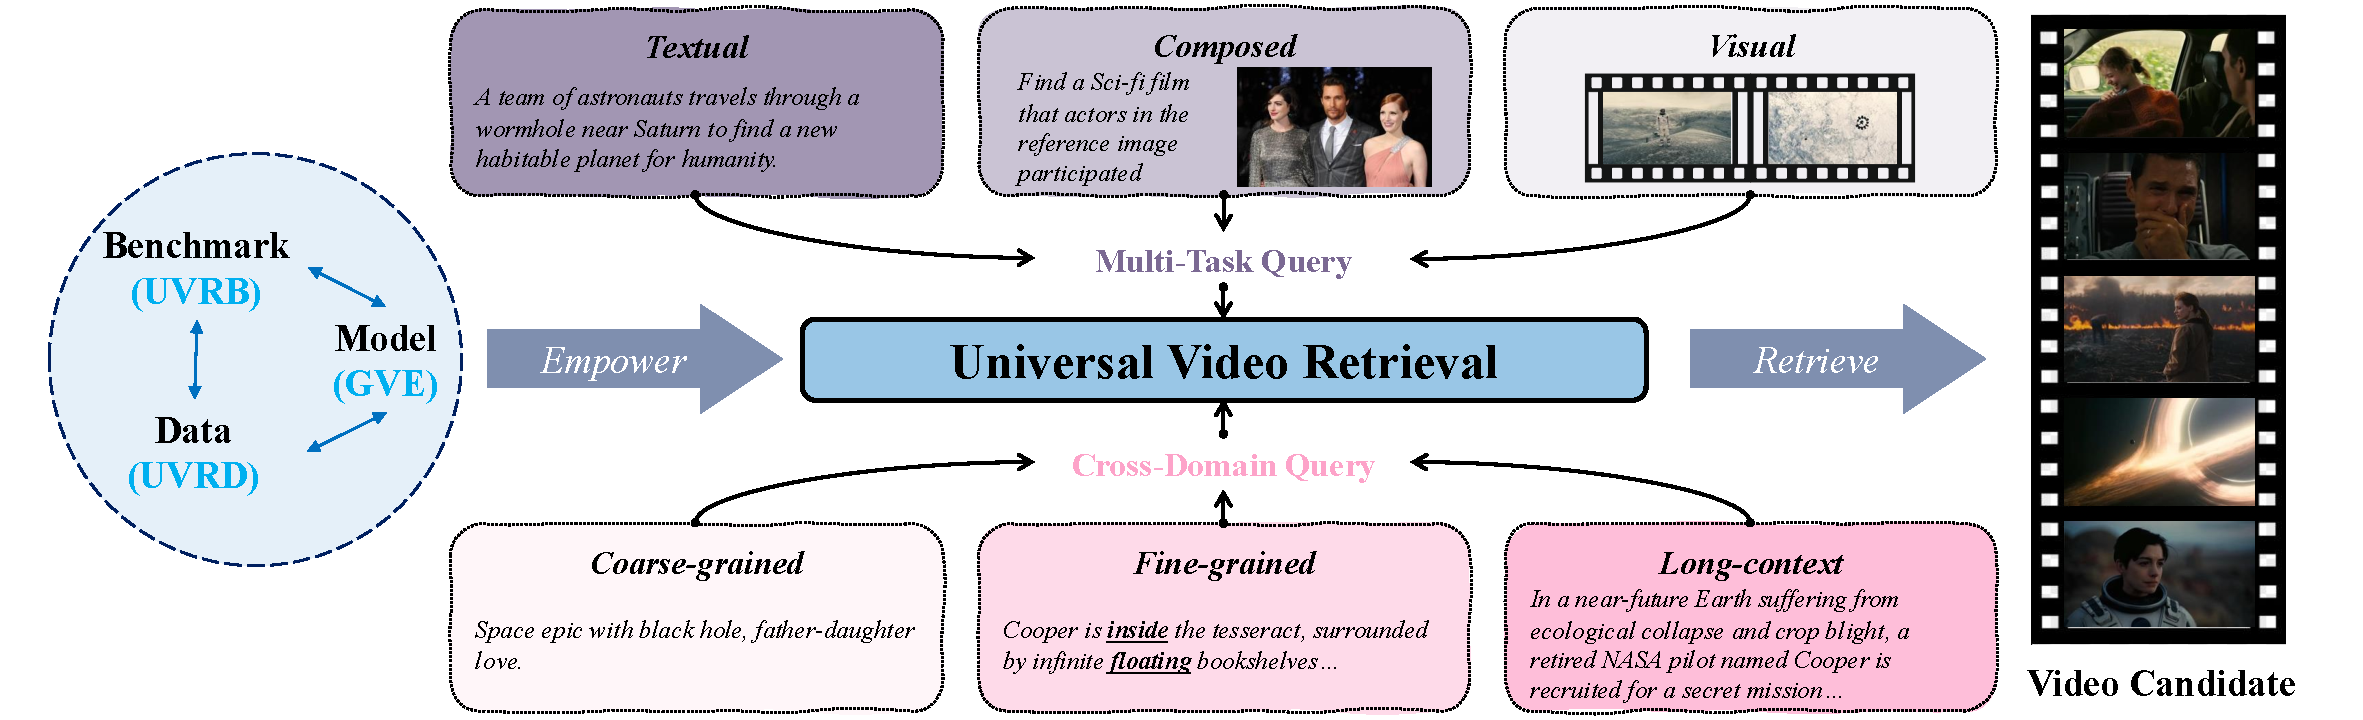
\includegraphics[width=\linewidth]{uvr.pdf}
    \caption{Universal Video Retrieval organizes heterogeneous retrieval settings into a unified capability space.}
    \label{fig:uvr}
\end{figure}

Therefore, to establish a framework for universal video retrieval that supports multi-domain, multi-granularity, and multi-task capabilities, \textit{two critical hurdles in data and modeling} must be addressed:  
(1)~\textit{Large-Scale Quality-Controlled Data Synthesis}: Existing datasets are either too small or are biased, while collecting a new, massive dataset is prohibitively expensive. Growing works attempt to synthesize data to address this challenge~\cite{chen2023vast,chai2024auroracap,ventura2024covr}. However, these resources often exhibit uneven quality and distribution. Therefore, gaining precise control over the properties of large-scale, cross-domain, multi-task data via a unified synthesis process is a primary challenge.  
(2)~\textit{Interconnected Multi-task Representation Learning}: A critical, often-ignored aspect is the inherent hierarchy among tasks. Foundational abilities such as spatial perception (e.g., object recognition) serve as building blocks for higher-order temporal reasoning (e.g., action recognition). This principle is evidenced by the remarkable success of image-only trained models like GME~\cite{Zhang_2025_CVPR} on video retrieval tasks (see Figure~\ref{gve:fig:radar_uvrb}), highlighting latent cross-task adaptability. Nevertheless, conventional models that assume task independence fail to capitalize on this structure, which is a key to unlocking superior generalization.

To this end, we propose a holistic framework that couples targeted data synthesis with stable modeling.  
First, to expose the concrete limitations of current approaches, we perform a standardized evaluation across $16$ established public datasets, assessing $14$ state-of-the-art models under unified preprocessing and metrics.  
Second, directly guided by the capability gaps identified in this evaluation (e.g., deficiencies in temporal and composed retrieval), we design \textbf{V-SynFlow}. This workflow transforms raw videos into a targeted, high-quality dataset, the \textbf{Universal Video Retrieval Dataset~(UVRD)}, consisting of over $1.55$ million multi-task pairs.  
Third, to ensure stability during heterogeneous training, we apply the \textbf{Modality Pyramid}, a training curriculum that leverages inherent task dependencies. It optimizes the \textbf{General Video Embedder (GVE)} by prioritizing foundational tasks before progressing to complex ones, facilitating smooth gradient convergence.

Extensive experiments validate the effectiveness of the GVE model~(Figure~\ref{gve:fig:radar_uvrb}). In addition to strong zero-shot performance, the analysis reveals that performance on conventional benchmarks correlates poorly with overall retrieval capability; meanwhile, partially relevant video retrieval can serve as a representative indicator of universal video retrieval.

\begin{figure}[t]
   \centering
   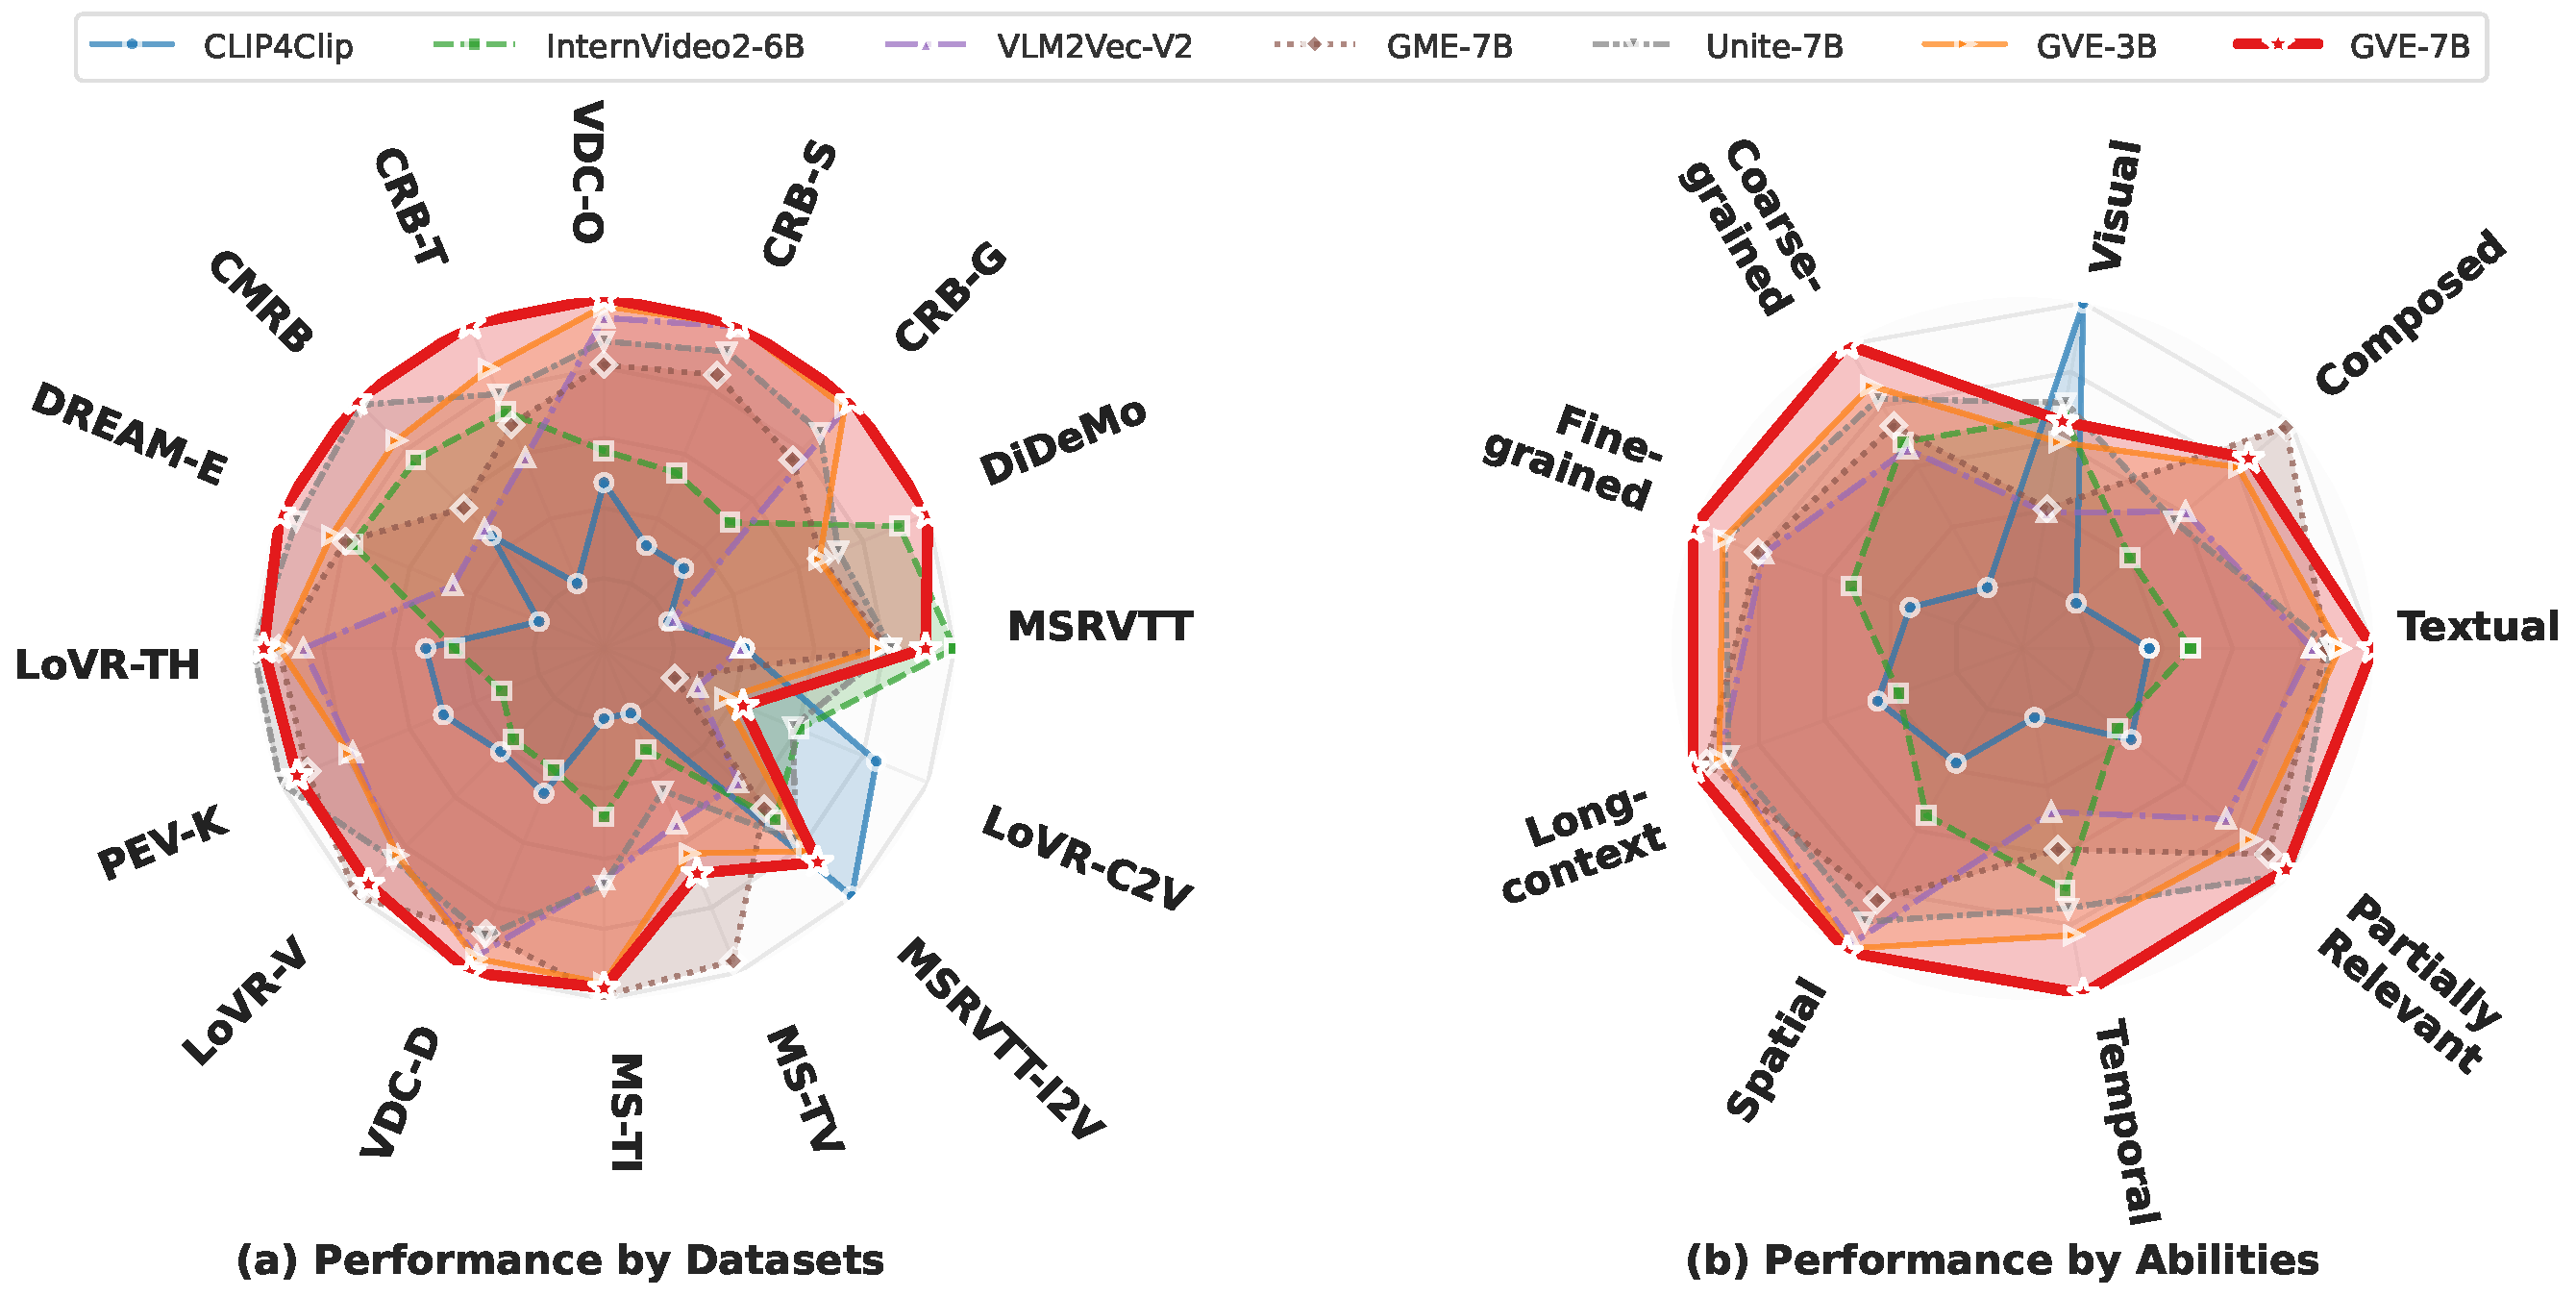
\includegraphics[width=\linewidth]{figures/gve/uvrb_dual_radar.pdf}
   \caption{Model performance on UVRB for 16 datasets and 9 abilities~(3 main tasks and 6 (sub-) domains).}
   \label{gve:fig:radar_uvrb}
\end{figure}

The contributions of this chapter are summarized as follows:
(1)~\textbf{Data}:~We propose V-SynFlow, a synthesis pipeline that produces UVRD with over $1.55$ million video-text pairs to explicitly address the data deficiencies identified in current models.
(2)~\textbf{Training}:~We introduce the Modality Pyramid curriculum, a training strategy that mitigates modality interference in heterogeneous multi-task learning, enabling the GVE model to achieve stable and strong zero-shot generalization.
(3)~\textbf{Analysis}:~Rather than proposing a novel benchmark, we establish a unified evaluation protocol across $16$ existing datasets. This standardized assessment systematically diagnoses model universality and offers new empirical insights beyond traditional evaluation paradigms.


\begin{figure}[t]
    \centering
    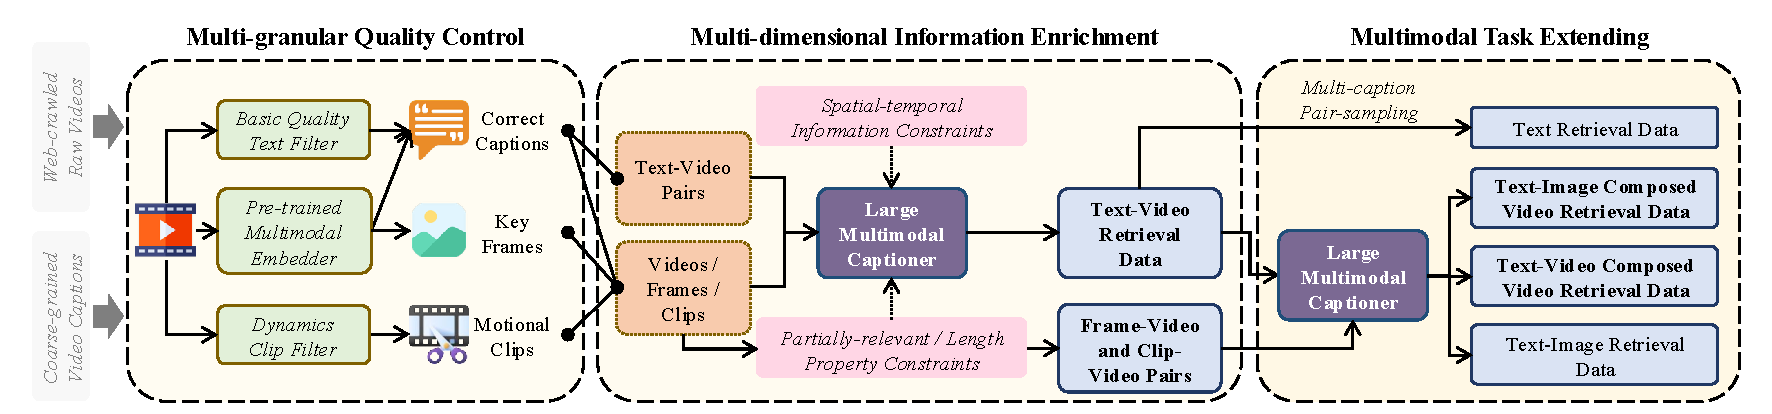
\includegraphics[width=\linewidth]{figures/gve/v-synflow.pdf}
    \caption{V-SynFlow: a multi-stage synthesis workflow for diverse video retrieval data.}
    \label{gve:fig:v-synflow}
\end{figure}

\section{Preliminary}\label{gve:sec:uvrb}

To bridge the persistent gap of fragmented evaluation protocols, we formulate the core problem from a holistic perspective by introducing the unified paradigm of Universal Video Retrieval~(UVR). This preliminary setup provides an objective diagnostic foundation to motivate our method contributions.

\subsection{Formulations}

The general ranking formulation in \S\ref{sec:bc-vr} is instantiated here across heterogeneous query formats and semantic domains. The query $q$, target video $v$, and cosine relevance score retain the meanings defined in Chapter~\ref{ch:related-work}. Here, the shared model $E_\theta$ instantiates the query and video embedding functions for heterogeneous inputs. UVR extends their scope by requiring consistent relevance ordering across the capability space defined below.

\begin{definition}[\textbf{Universal Video Retrieval~(UVR)}]\label{gve:def:universal_video_retrieval}
    Given a matching pair comprising a query $q$ and a video $v$, UVR aims to learn a $\theta$-parameterized model $E_\theta(\cdot)$ to compute a relevance score $s_{q \to v} = \cos(E_\theta(q), E_\theta(v))$. This score must be consistently higher than the similarity scores of irrelevant pairs across the query formats and data domains in the capability space defined below.
    Specifically, this paradigm categorizes the retrieval space into two primary dimensions:
    \textbf{(1)~Query Format} incorporates Textual~(TXT, e.g., natural language), Composed~(CMP, combinations such as text and image or text and video), and Visual~(VIS, pure image or video queries).
    \textbf{(2)~Data Domain} incorporates Coarse-grained~(CG, high-level semantics), Fine-grained categories including Spatial~(S, object), Temporal~(T, dynamics), and Partially Relevant~(PR, partial information), alongside Long-context~(LC, lengthy inputs).
\end{definition}

This formalization integrates isolated retrieval tasks into a comprehensive taxonomy, delineating the full spectrum of capabilities required for a truly universal video retrieval system.

\subsection{Unified Evaluation Protocol}

To operationalize the UVR paradigm and systematically diagnose generalization bottlenecks, we establish a standardized evaluation protocol across $16$ public video retrieval datasets. The consolidation of these existing resources into a unified evaluation suite, which we refer to as the Universal Video Retrieval Benchmark~(UVRB) protocol, provides a comprehensive framework for assessing model universality against the exhaustive query formats and domain complexities outlined in Definition~\ref{gve:def:universal_video_retrieval}.

To guarantee an objective assessment, all datasets undergo identical preprocessing, including uniform frame sampling, query normalization per task type, and strict adherence to a vision-only input scope. The evaluation follows a strictly model-agnostic protocol. Embeddings are extracted directly from the frozen representation space, and relevance is computed solely via cosine similarity without task-specific post-processing or learnable projections. This standardization eliminates heuristics and isolates the visual-semantic alignment capabilities of the backbones.

This comprehensive diagnostic framework exposes systemic capability deficiencies across current models, directly motivating the targeted data synthesis pipeline and heterogeneous task curriculum introduced in the subsequent methodology. The benchmark composition, dataset preparation, and execution pipeline are detailed below.

\subsubsection{Benchmark Composition and Dataset Preparation}

Figure~\ref{gve:fig:uvrb} visualizes how the 16 datasets cover the UVR capability space. Table~\ref{gve:tab:uvrb_dataset} summarizes their query and corpus sizes, video durations, and text lengths. All videos are evaluated using eight uniformly sampled frames. The datasets are grouped by query format and semantic domain according to Definition~\ref{gve:def:universal_video_retrieval}.

\begin{figure}[t]
    \centering
    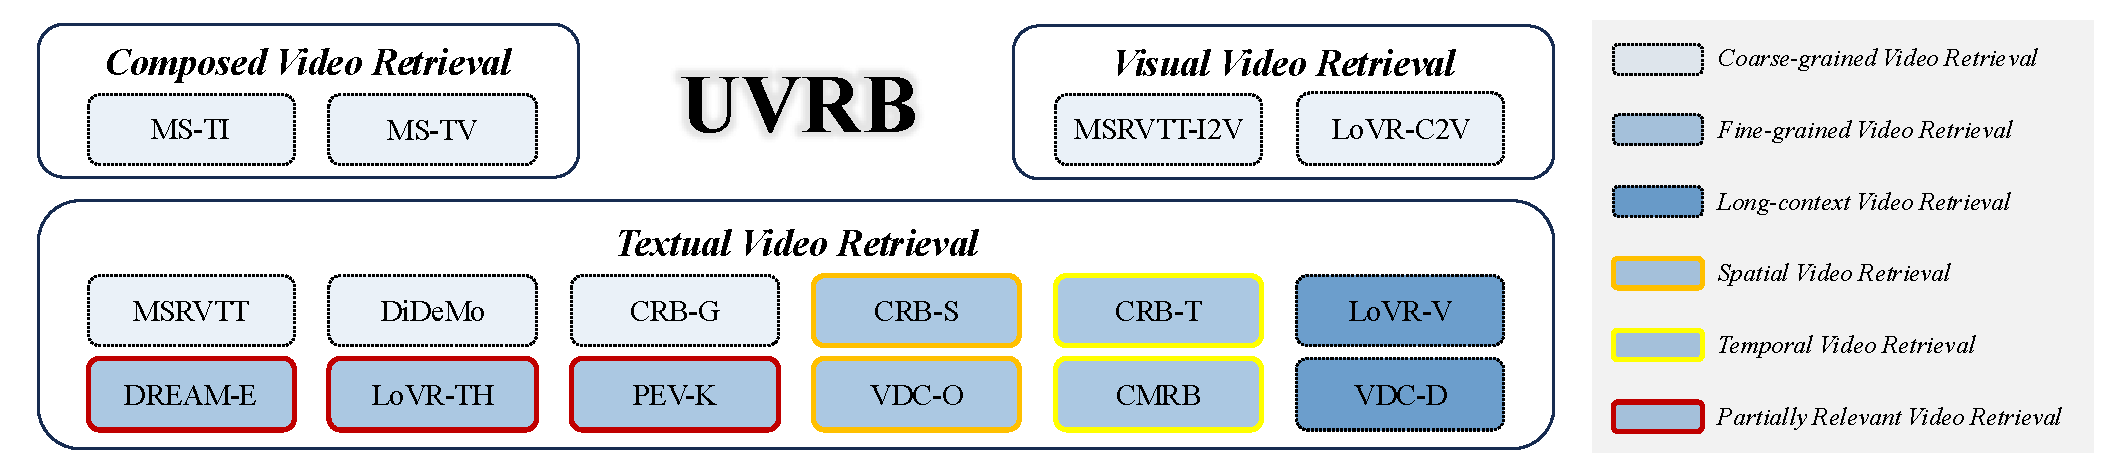
\includegraphics[width=\linewidth]{figures/gve/uvrb.pdf}
    \caption{Organization of the 16 public datasets in UVRB by query format and retrieval capability.}
    \label{gve:fig:uvrb}
\end{figure}

\begin{table}[t]
\centering
\caption{Statistics of the datasets in UVRB. All videos use eight uniformly sampled frames. Dur. denotes duration in seconds, and \# Word denotes query length in words.}
\label{gve:tab:uvrb_dataset}
\begin{tabular}{l r r r r}
\toprule
\textbf{Dataset} & \textbf{\# Query} & \textbf{\# Corpus} & \textbf{Dur.} & \textbf{\# Word} \\
\midrule
\multicolumn{5}{l}{\textbf{Textual Video Retrieval (Coarse-grained)}} \\
MSRVTT~\cite{xu2016msr} & 1,000 & 1,000 & 15.0 & 9.4 \\
DiDeMo~\cite{anne2017localizing} & 1,004 & 1,004 & 53.9 & 29.1 \\
CaReBench-General (CRB-G)~\cite{xu2025carebench} & 1,000 & 1,000 & 14.4 & 232.2 \\
\midrule
\multicolumn{5}{l}{\textbf{Textual Video Retrieval (Fine-grained Spatial)}} \\
CaReBench-Spatial (CRB-S)~\cite{xu2025carebench} & 1,000 & 1,000 & 14.4 & 115.0 \\
VDC-Object (VDC-O)~\cite{chai2024auroracap} & 1,027 & 1,027 & 30.1 & 91.4 \\
\multicolumn{5}{l}{\textbf{Textual Video Retrieval (Fine-grained Temporal)}} \\
CaReBench-Temporal (CRB-T)~\cite{xu2025carebench} & 1,000 & 1,000 & 14.4 & 103.2 \\
CameraBench (CMRB)~\cite{lin2025towards} & 728 & 1,071 & 5.7 & 24.8 \\
\multicolumn{5}{l}{\textbf{Textual Video Retrieval (Partially Relevant)}} \\
DREAM-1K-Event (DREAM-E)~\cite{wang2024tarsier} & 6,251 & 1,000 & 8.8 & 6.5 \\
LoVR-Theme2Clip (LoVR-TH)~\cite{cai2025lovr} & 8,854 & 8,854 & 16.9 & 48.1 \\
PE-Video-Keyword (PEV-K)~\cite{bolya2025perception} & 14,427 & 15,000 & 16.9 & 45.5 \\
\midrule
\multicolumn{5}{l}{\textbf{Textual Video Retrieval (Long-context)}} \\
LoVR-Text2Video (LoVR-V)~\cite{cai2025lovr} & 100 & 467 & 1560.3 & 17364.5 \\
VDC-Detail (VDC-D)~\cite{chai2024auroracap} & 1,000 & 1,027 & 30.1 & 508.0 \\
\midrule
\multicolumn{5}{l}{\textbf{Composed Video Retrieval}} \\
MomentSeeker-Text-Image (MS-TI)~\cite{yuan2025momentseeker} & 400 & 10 & 13.5 & 68.5 \\
MomentSeeker-Text-Video (MS-TV)~\cite{yuan2025momentseeker} & 400 & 10 & 13.5 & 68.5 \\
\midrule
\multicolumn{5}{l}{\textbf{Visual Video Retrieval}} \\
MSRVTT-ImageVideo (MSRVTT-I2V)~\cite{xu2016msr} & 1,000 & 1,000 & 15.0 & -- \\
LoVR-Clip-to-Video (LoVR-C2V)~\cite{cai2025lovr} & 467 & 467 & 1560.3 & -- \\
\bottomrule
\end{tabular}
\end{table}

We use the JSFusion split of MSRVTT~\cite{yu2018joint} and concatenate all descriptions of each DiDeMo video following~\cite{liu2019use}. For CaReBench, the general, spatial, and temporal caption fields define CRB-G, CRB-S, and CRB-T, respectively. VDC-O uses the object-centric captions from VDC, while CMRB uses camera-motion descriptions. DREAM-E, LoVR-TH, and PEV-K use event descriptions, theme annotations, and keyword fields to evaluate partially relevant retrieval. LoVR-V and VDC-D use long-form and detailed captions for long-context retrieval. Following the MomentSeeker adaptation in~\cite{meng2025vlm2vec}, MS-TI and MS-TV combine text with an image or a video clip to retrieve a target clip. For visual retrieval, MSRVTT-I2V uses one randomly sampled frame as the query, and LoVR-C2V uses a short clip to retrieve its source long video.

Table~\ref{gve:tab:uvrb_prompts_metric} lists the instruction and metric for each dataset. This explicit mapping keeps instruction-sensitive models under a common task definition while preserving the metric appropriate to each benchmark.

\begin{table}[t]
\centering
\caption{Query instructions and metrics for the datasets in UVRB.}
\label{gve:tab:uvrb_prompts_metric}
\begin{tabular}{l p{10cm} l}
\toprule
\textbf{Dataset} & \textbf{Query Instruction} & \textbf{Metric} \\
\midrule
MSRVTT & Find the clip that corresponds to the described scene in the given video. & R@1 \\
DiDeMo & Find a video that includes the following described scenes. & R@1 \\
CRB-G & Find the video according to the general text description. & R@1 \\
CRB-S & Find the video according to the spatial description. & R@1 \\
VDC-O & Find the video according to the object description. & R@1 \\
CRB-T & Find the video according to the temporal description. & R@1 \\
CMRB & Find the video according to the camera motion description. & R@10 \\
DREAM-E & Find the video according to the text description. & R@1 \\
LoVR-TH & Find the video according to text description about video theme information. & R@10 \\
PEV-K & Find the video according to the text description of a series of keywords. & R@1 \\
LoVR-V & Find the long video according to the long text description. & R@1 \\
VDC-D & Find the video according to the detailed text description. & R@1 \\
MS-TI & Find the video clip that corresponds to the given text and image. & P@1 \\
MS-TV & Find the video clip that corresponds to the given text and video. & P@1 \\
MSRVTT-I2V & Find the video according to the image. & R@1 \\
LoVR-C2V & Find the original long video according to the short video clip. & R@1 \\
\bottomrule
\end{tabular}
\end{table}

\subsubsection{Evaluation Pipeline}

The evaluation is implemented on MTEB~\cite{muennighoff2022mteb} and decouples the evaluation engine from the model architecture through a standardized interface. It proceeds through dynamic task orchestration, configurable model execution, and metric and diagnostic generation. Domain-specific prompts are injected for instruction-sensitive tasks, while dedicated loaders integrate custom benchmarks. Expensive tasks can be deferred, and model initialization abstracts precision and multi-GPU configuration. The data layer supports online and offline modes, and explicit multi-GPU management and clean shutdown handling improve reliability for large-scale evaluation.


\section{Methodology}

This section introduces a co-designed framework for universal video retrieval. Guided by UVR, we first propose V-SynFlow. This workflow synthesizes the Universal Video Retrieval Dataset~(UVRD), comprising $1.55$ million targeted video-text pairs to explicitly supplement general retrieval data. Subsequently, we introduce the \pyramid curriculum, a strategy designed to stabilize the optimization of the General Video Embedder~(GVE) by leveraging inherent task hierarchies across heterogeneous modalities.

\subsection{Scalable Synthesis of Cross-Domain Multi-Task Video Retrieval Data}\label{gve:sec:data_synthesis}
Training a universal video embedder is fundamentally impeded by a deficiency of high-quality supervision for divergent tasks. Guided by the concrete capability gaps identified in the preliminary diagnostics, such as severe shortcomings in fine-grained temporal reasoning and composed retrieval, we introduce \textbf{V-SynFlow}~(Figure~\ref{gve:fig:v-synflow}). This pipeline transforms weakly annotated web videos from raw datasets~(e.g., PVD~\cite{bolya2025perception}, InternVid-FLT~\cite{wang2023internvid}, and WebVid~\cite{bain2021frozen}) into structured, high-fidelity, and gap-targeted multi-task training instances. Through this targeted approach, we construct the \textbf{Universal Video Retrieval Dataset~(UVRD)}, containing over $1.55$ million descriptive pairs tailored for multidimensional training enhancement.
Specifically, the V-SynFlow workflow proceeds in three stages as follows. The construction implementation and complete generation prompts are provided after the three stages.

\paragraph{Multi-granular Quality Control.}
Given a raw corpus $\mathcal{D} = \{(v_i, t_i)\}$, we produce a high-fidelity asset pool, $\mathcal{A}_{tfc}$. The process applies a filter cascade. \textit{Annotation Rectification} removes non-descriptive text. \textit{Cross-Modal Consistency Filtering} discards pairs where the similarity measured by a pretrained embedder $\Phi(\cdot)$~(e.g., GME-7B~\cite{Zhang_2025_CVPR}) falls below a predefined threshold, empirically set to 0.25. \textit{Temporal Dynamics Filtering} removes static content to ensure sufficient temporal signals. The resulting asset pool $\mathcal{A}_{tfc}$ contains a set of validated videos $\{v_j\}$, the original captions $\{t_j\}$, and corresponding sets of extracted frames $\{f_{jk}\}$ alongside cropped clips $\{c_{jl}\}$.

\begin{figure}[t]
    \centering
    \begin{minipage}[b]{0.7\textwidth}
        \centering
        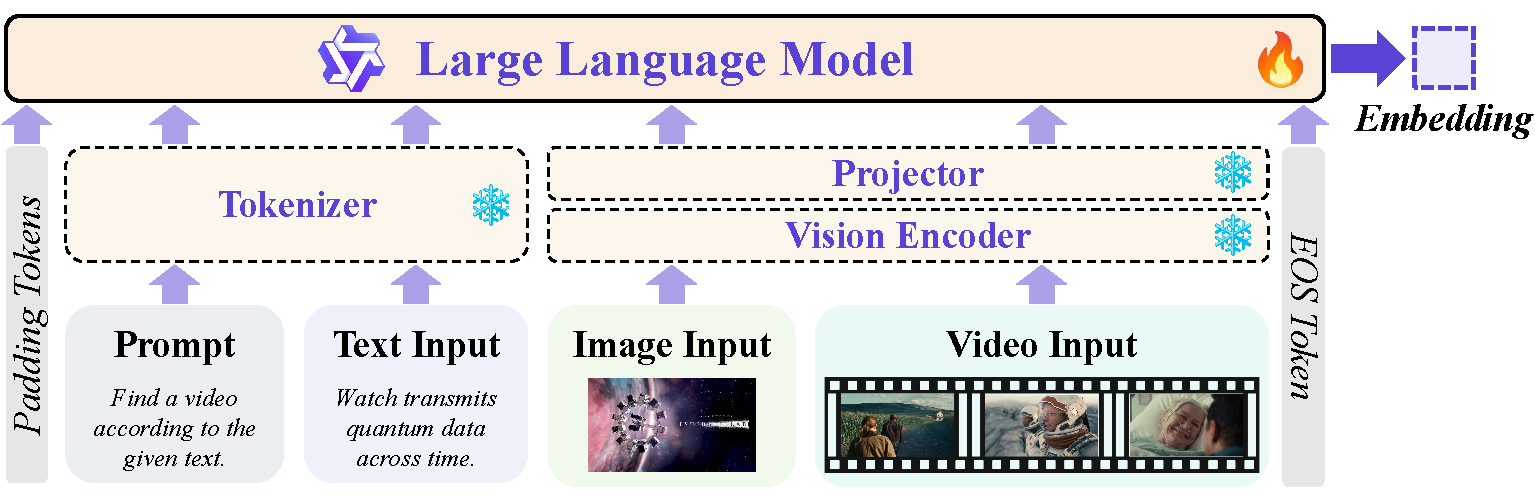
\includegraphics[width=\linewidth]{figures/gve/model.pdf}
        \caption{The architecture of GVE, an MLLM-based embedding model. We fine-tune only the LLM component. GVE accepts compositional multimodal inputs and produces a high-dimensional embedding.}
        \label{gve:fig:model}
    \end{minipage}
    \hfill
    \begin{minipage}[b]{0.26\textwidth}
        \centering
        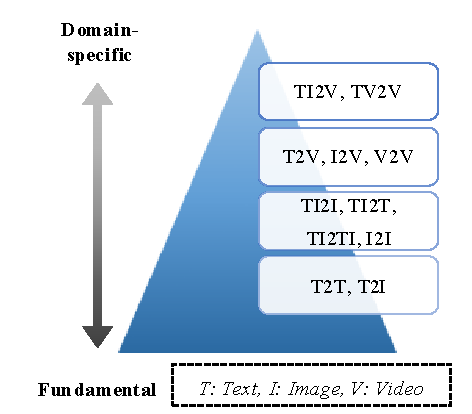
\includegraphics[width=\linewidth]{figures/gve/modality-pyramid.pdf}
        \caption{\pyramid: simpler tasks lay the foundation for specific ones.}
        \label{gve:fig:pyramid}
    \end{minipage}
\end{figure}

\paragraph{Multi-dimensional Information Enrichment.}
We leverage the filtered assets within $\mathcal{A}_{tfc}$ to generate richer data structures. To create an enriched text-video dataset $\mathcal{D}^{+}$, we utilize an MLLM, $\mathcal{M}_{\text{cap}}$~(e.g., Keye-VL-8B~\cite{team2025kwai}), as a conditional captioning engine. For each video $v_j$, the engine synthesizes multiple captions $\{t^{'}_{jk}\}$ conditioned by diagnostic-driven information profiles. Specifically, because the diagnostic evaluation revealed a pronounced spatial-temporal decoupling wherein temporal skills constitute the primary bottleneck, we deliberately skew the synthesis distribution: $60\%$ temporal, $30\%$ spatial, and $10\%$ targeted at partially relevant or abstract semantics, informed by our preliminary diagnostic results on UVRB. By sampling one caption for each video, we obtain a set of novel high-quality text-video pairs $\{(v_j, t^{'}_{jk})\}$. Furthermore, we pair videos with the corresponding visual components to construct collections of visual pairs $\mathcal{P}_{f \leftrightarrow v}$ and $\mathcal{P}_{c \leftrightarrow v}$, resulting in frame-to-video $\{(f_{jk}, v_j)\}$ and clip-to-video $\{(c_{jl}, v_j)\}$ instances. To mitigate potential hallucination biases inherent in generative MLLMs, we enforce strict instructional prompts and rely on the aforementioned cross-modal consistency filtering to automatically discard misaligned generations.

\paragraph{Multimodal Task Extension.}
The final stage assembles the unified training corpus, $\mathcal{D}_{\star}$. To explicitly address the composed retrieval deficiency, we synthesize complex composed tasks by leveraging $\mathcal{P}_{f \leftrightarrow v}$ and $\mathcal{P}_{c \leftrightarrow v}$. For each visual pair, such as $(f_{jk}, v_j)$, the engine $\mathcal{M}_{\text{cap}}$ generates a query text $t^{f_{jk} \to v_j}$ describing the temporal evolution, forming a training instance $((t^{f_{jk} \to v_j}, f_{jk}), v_j)$. Additionally, basic alignment tasks (e.g., text-image pairs) are sampled from $\mathcal{A}_{tfc}$. For each video, two candidates from the unselected synthesized captions are mapped as text-to-text pairs. The resulting dataset $\mathcal{D}_{\star}$ provides the comprehensive mixture of tasks essential for training a universal embedder.

\paragraph{Dataset-Construction Implementation.}
To support scalable and reproducible construction across these task types, we implement V-SynFlow as a unified object-oriented framework. Every retrieval task is represented by a canonical tripartite abstraction comprising a \textsc{Corpus}, a set of \textsc{Queries}, and a \textsc{Relevance Mapping}. An abstract base class enforces this structural invariant across text-to-video, visual, and composed retrieval datasets.

The framework supports three forms of specialization. First, modality is treated as configuration, allowing a dataset to transition among text, image, video, and composite queries by overriding its modality-specific access method. Second, complex tasks are derived through inheritance. For example, a text-and-image-to-video task extends a base retrieval task with an additional query component, while dataset variants override only the required data-access methods. Third, large sources such as InternVid-FLT are processed in parallel chunks, with automated validators checking resolution, frame count, and video integrity. Common media errors are repaired using \texttt{ffmpeg}, reducing the risk that downstream failures originate from corrupted input rather than retrieval difficulty.

\subsubsection{Prompt Specifications for Synthetic Data Generation}\label{gve:sec:prompt_specs}

To ensure high-quality, diverse, and controllable synthetic video retrieval data generation at scale, we design and deploy a suite of structured prompts to instruct MLLMs for captioning. Our pipeline operates in four parts:

\begin{enumerate}
    \item \textbf{Raw~(Or Weakly Annotated) Video (Re-)~Captioning}: Enhance raw or uncaptioned videos with rich, diverse textual descriptions.
    \item \textbf{Text-Image Composed Retrieval}: Generate queries that combine reference images with video content for fine-grained retrieval.
    \item \textbf{Text-Video Composed Retrieval}: Generate queries that combine short reference clips with target videos for practical temporal or perspective-based retrieval.
    \item \textbf{Frame Image Captioning}: Annotate individual video frames with dynamic-aware captions for auxiliary training signals.
\end{enumerate}

All prompts enforce strict output formatting, factual grounding, and stylistic diversity to ensure dataset quality and coverage. \texttt{\{raw\_caption\}} represents an optional, potentially low-quality human-provided or auto-generated caption associated with the video. Placeholders (e.g., \texttt{\{readability\}} and \texttt{\{education\_level\}}) are dynamically instantiated during batch generation.

We also generate text-to-text retrieval data by randomly pairing two descriptions from the video or frame caption list.

% ========================================
% Prompt 1: Video Captioning
% ========================================
\begin{promptbox}{Synthetic Video Captioning Prompt}
\begin{lstlisting}[style=promptstyle]
Generate 5 distinct and high-quality ENGLISH captions for the provided video. Please first visually understand the video file and analyze the video frame-by-frame in depth before captioning.

The original video caption is {raw_caption}. (Ignore if empty.)

Each caption must be:
  1. The final answer MUST only be a JSON dict of captions where the key is the caption number and the value is a single-paragraph caption.
  2. Factually accurate and descriptive - include only what is clearly visible or reasonably inferable from the video.
  3. Focus exclusively on visible content; do not mention absences or speculate about unseen elements.

Content Requirements (per caption):
  1. Spatial Details (30-60%): Describe location, setting, key environmental elements, objects, and their spatial relationships. Include notable visual features.
  2. Temporal Flow (30-60%): Capture event sequence and action dynamics - movements, interactions, transitions - as they unfold over time.
  3. Theme/Background/Style/Meaning/Highlight/Camera (0-20%): Describe observable emotional tone, narrative style, thematic elements, highlighting frames, or significant camera movements/angles.
  4. Others (0-10%).

Key Guidelines:
  1. Do not invent fictional elements, dialogue, or backstory not visible in the video.
  2. Use the following varied sentence styles (one per caption):
       - concise and punchy summary,
       - spatial-temporal richly descriptive,
       - abstract understanding,
       - keywords-only,
       - partially relevant information.
  3. Ensure diversity: avoid repetition in wording, focus, or rhythm; at least one caption must be <20 words and one >100 words; balance objectivity with vivid sensory language; randomly omit minor details in 1 or 2 captions.
  4. Ensure readability matches {readability} and is appropriate for {education_level} readers.

Now generate these captions in strict JSON format:
{
   "1": <caption text 1: concise and punchy summary, 10-25 words>,
   "2": <caption text 2: spatial-temporal richly descriptive, 80-200 words>,
   "3": <caption text 3: abstract understanding, 30-100 words>,
   "4": <caption text 4: keywords-only, 5-30 words>,
   "5": <caption text 5: partially relevant information, 10-70 words>
}
\end{lstlisting}
\end{promptbox}

% ========================================
% Prompt 2: Text-Image Composed Retrieval
% ========================================
\begin{promptbox}{Synthetic Text-Image Composed Video Retrieval Prompt}
\begin{lstlisting}[style=promptstyle]
You are an information retrieval expert specializing in high-value text-image composed queries. Your sole objective is to generate queries that significantly enhance video retrieval performance by effectively combining a reference image and video content.

## What Makes a HIGH-QUALITY Query (Non-Negotiable)
A truly valuable query must satisfy ALL of these criteria:

1. COMBINATION NECESSITY (Most Critical)
   - The query MUST become meaningless or significantly less specific if either the image or video is removed.
   - Example (HIGH-QUALITY): "the person FROM REFERENCE IMAGE wearing red jacket now skiing"
   - Example (LOW-QUALITY): "a person skiing" (works without image)

2. SEMANTIC PRECISION
   - Must accurately reflect BOTH the visual content of the reference image AND the video.
   - Must reference at least ONE specific visual attribute from the image (not generic descriptions).
   - Example (HIGH-QUALITY): "matching the blue hat FROM PHOTO, now running through park"
   - Example (LOW-QUALITY): "someone similar to image moving" (too vague)

3. RETRIEVAL EFFECTIVENESS
   - Must narrow search results by at least 50\% compared to text-only queries.
   - Must contain actionable constraints that differentiate from 90\% of videos in the database.
   - Example (HIGH-QUALITY): "the woman WITH PONYTAIL FROM IMAGE entering building at 2PM"
   - Example (LOW-QUALITY): "a woman walking" (too broad)

4. LOGICAL COHERENCE
   - Must maintain subject-verb-object consistency across modalities.
   - Must avoid semantic contradictions between image attributes and video actions.
   - Example (HIGH-QUALITY): "the dog FROM REFERENCE PHOTO chasing a ball"
   - Example (LOW-QUALITY): "the red jacket FROM IMAGE running down hill" (jackets don't run)

5. PRACTICAL UTILITY
   - Must solve a real-world ambiguity that neither text nor image could resolve alone.
   - Must reflect how actual users would express their information need.
   - Example (HIGH-QUALITY): "same person AS IN PHOTO but wearing blue instead of red"
   - Example (LOW-QUALITY): "the image shows a person and the video shows action" (no real combination)

## High-Value Query Generation Framework
Follow this structured approach:

1. DEEP ANALYSIS PHASE (Mandatory)
   a) Reference Image Analysis:
      - Identify 1-4 SPECIFIC visual attributes (e.g., "red jacket", "ponytail", "blue hat")
      - Determine primary subject with discriminative features
      - Note what CANNOT be determined from image (e.g., action, scene)

   b) Video Content Analysis:
      - Identify primary action using precise verbs (e.g., "running", "entering", "chasing")
      - Note scene context and temporal elements
      - Determine what CHANGES from the static image reference

2. COMBINATION STRATEGY SELECTION
   Choose ONE primary strategy:

   A) IDENTITY PRESERVATION + ACTION CHANGE
      - Structure: [Binding phrase] + [Image attribute] + [Video action]
      - Example: "the man FROM REFERENCE IMAGE in blue shirt now running"

   B) IDENTITY PRESERVATION + SCENE MIGRATION
      - Structure: [Binding phrase] + [Image attribute] + [Scene transition]
      - Example: "same person AS IN PHOTO moving from office to park"

   C) IDENTITY PRESERVATION + NEGATIVE CONSTRAINT
      - Structure: [Binding phrase] + [Negative constraint] + [Video state]
      - Example: "not wearing red jacket FROM IMAGE but blue, walking"

   D) RELATIONAL TRANSFER
      - Structure: [Binding phrase] + [Relationship description]
      - Example: "the dog FROM REFERENCE PHOTO chasing a ball"

3. QUALITY ENHANCEMENT TECHNIQUES
   - Binding Precision: Use "FROM REFERENCE IMAGE", not "like the picture"
   - Attribute Specificity: Use concrete features ("red jacket", not "clothing")
   - Action Verbs: Use present continuous tense ("running", not "runs")
   - Context Enrichment: Add 1 relevant scene descriptor ("in park", "near building")
   - Noise Handling: For low-quality inputs, use "resembling" but maintain specificity
   - Audience Adaptation: Ensure readability matches {readability} and suits {education_level} readers.

4. MANDATORY QUALITY CHECK
   Before finalizing, verify ALL:
   - [ ] Explicit binding to reference image
   - [ ] References SPECIFIC visual attribute from image
   - [ ] Describes DYNAMIC ELEMENT not in static image
   - [ ] Loses specificity if image removed
   - [ ] Contains actionable retrieval constraint
   - [ ] Maintains logical subject-action consistency
   - [ ] Solves real-world ambiguity

## What to AVOID
- Generic descriptions ignoring image specificity
- Redundant mentions of obvious image content
- Semantic contradictions (e.g., "the jacket is running")
- Overly precise details not visible in inputs
- Standalone video descriptions without image binding
- Vague terms: "something", "thing", "area"
- Excessive length without added value (>50 words)

## Output Format
- Output ONLY a JSON object with one key: "query"
- Value must be the generated query sentence
- No additional text or formatting

Generate the query for:
Reference Image: <image_input>
Video Clip: <video_input>
\end{lstlisting}
\end{promptbox}

% ========================================
% Prompt 3: Text-Video Composed Retrieval
% ========================================
\begin{promptbox}{Synthetic Text-Video Composed Video Retrieval Prompt}
\begin{lstlisting}[style=promptstyle]
You are an information retrieval expert specializing in practical text-video composed queries. Your objective is to generate queries that effectively combine a short reference clip with a target video for real-world retrieval.

## Practical Context Understanding
In real-world scenarios:
- Reference is typically a SHORT CLIP (2-10 seconds)
- Clip is usually HIGHLY RELEVANT to target video (same source or similar content)
- Common relationships: temporal continuation, perspective variation, quality differences, minor action variations
- Query should reflect how users actually search

## What Makes a HIGH-QUALITY Query (Practical Focus)
Must satisfy these criteria:

1. USEFUL COMBINATION (Most Important)
   - Leverages reference clip to specify what text alone cannot
   - Example (HIGH-QUALITY): "the same person FROM REFERENCE CLIP continuing to run after the jump"
   - Example (LOW-QUALITY): "a person running" (ignores reference)

2. PRACTICAL PRECISION
   - References at least ONE observable feature from reference clip
   - Example (HIGH-QUALITY): "matching the red jacket FROM REFERENCE, now entering building"
   - Example (LOW-QUALITY): "someone similar to clip moving" (too vague)

3. REAL-WORLD UTILITY
   - Helps find videos difficult to retrieve with text alone
   - Example (HIGH-QUALITY): "same action AS IN REFERENCE but from front angle"
   - Example (LOW-QUALITY): "the clip shows action" (no retrieval value)

4. NATURAL EXPRESSION
   - Sounds like how a real user would phrase it
   - Example (HIGH-QUALITY): "what happens right after this moment?"
   - Example (LOW-QUALITY): "temporal continuation of the current visual sequence" (too academic)

## Practical Query Generation Framework

1. REFERENCE CLIP ANALYSIS
   - Identify 1-3 KEY OBSERVABLE FEATURES (e.g., "red jacket", "starting pose", "mid-action")
   - Determine most distinctive visual or action element
   - Note what is CLEARLY VISIBLE (avoid guessing)

2. TARGET VIDEO RELATIONSHIP ASSESSMENT
   Determine relationship type:

   A) TEMPORAL CONTINUATION
      - Reference is earlier part of same sequence
      - Query focus: "what happens next" or "continuing action"

   B) PERSPECTIVE VARIATION
      - Same action from different angle/view
      - Query focus: "same action from different angle"

   C) QUALITY/CONDITION VARIATION
      - Same action with different lighting/resolution
      - Query focus: "same scene in better lighting"

   D) MINOR ACTION VARIATION
      - Slightly different execution of similar action
      - Query focus: "same person but running instead of walking"

3. QUERY CONSTRUCTION
   - Start with binding phrase: "FROM REFERENCE CLIP", "AS IN REFERENCE", etc.
   - Reference 1-2 specific observable features from clip
   - Describe relationship to target video clearly
   - Keep natural and practical (5-15 words typically)
   - For temporal: focus on "what happens next"
   - For perspective: specify desired viewpoint
   - For quality: specify desired condition
   - For action: specify the change

4. PRACTICAL QUALITY CHECK
   Ask before finalizing:
   - Would this help me find what I'm looking for?
   - Does it add value beyond describing the target?
   - Would a real user phrase it this way?
   - Is everything mentioned clearly visible in reference?

## What to AVOID
- Overly academic or technical language
- References to features NOT clearly visible
- Excessive precision about timing ("exactly 3.2 seconds later")
- Queries that work equally well without reference
- Generic descriptions: "similar video", "related content"
- Making unsupported assumptions

## Output Format
- Output ONLY a JSON object with key: "query"
- Value must be the generated query string
- No additional text, explanations, or formatting

Generate the query for:
Reference Clip: <reference_clip_input>
Target Video: <target_video_input>
\end{lstlisting}
\end{promptbox}

% ========================================
% Prompt 4: Frame Captioning
% ========================================
\begin{promptbox}{Synthetic Frame Captioning Prompt}
\begin{lstlisting}[style=promptstyle]
Generate 5 distinct and high-quality ENGLISH captions for the provided image (a frame extracted from a video) based solely on visual content. Please first visually understand the image and analyze it in depth before captioning.

Each caption must be:
  1. The final answer MUST only be a JSON dict of captions where the key is the caption number and the value is a single-paragraph caption.
  2. Factually accurate and descriptive - include only what is clearly visible; captions should also be consistent with the short-term video context.
  3. Focus exclusively on visible content; do not mention absences or speculate about unseen context.

Content Requirements (per caption):
  1. Spatial Details (50-70%): Describe location, setting, key objects, spatial relationships, colors, lighting, composition. Include instantaneous action states derived from visible posture/motion cues.
  2. Temporal Snapshots (0-30%): Describe the frozen moment's temporal state (movements, interactions, transitions) ONLY if visually provable. Avoid implying sequence, duration, or speed.
  3. Theme/Style/Composition (10-20%): Cover emotional tone, camera angle, lighting style, or artistic elements directly observable.
  4. Others (0-10%).

Key Guidelines:
  1. Do not invent fictional elements or backstory. If action is ambiguous, describe neutrally. Never use future/past tense or speculative phrases.
  2. Use varied sentence styles (randomly assign one per caption):
       - concise spatial-temporal snapshot,
       - spatially rich descriptive,
       - abstract spatial interpretation,
       - keywords with temporal anchors,
       - minimalist spatial focus.
  3. Ensure diversity: avoid repetition in wording, focus, or rhythm; at least one caption <20 words and one >100 words; balance objectivity with vivid sensory language; randomly omit minor details in 1-2 captions.
  4. Ensure readability matches {readability} and is appropriate for {education_level} readers.

Now generate these captions in strict JSON format:
{
   "1": <caption text 1: concise and punchy summary, 10-25 words>,
   "2": <caption text 2: spatial-temporal richly descriptive, 50-200 words>,
   "3": <caption text 3: abstract understanding, 30-100 words>,
   "4": <caption text 4: keywords-only, 5-30 words>,
   "5": <caption text 5: partially relevant information, 10-70 words>
}
\end{lstlisting}
\end{promptbox}

\paragraph{Prompt Utilization.}
These prompts are designed for a scalable, schema-constrained generation pipeline for synthesizing diverse video-centric annotations and queries. The system unifies four tasks under a single modular framework.
Each task is governed by a structured prompt template with dynamic control slots (e.g., readability, education level), ensuring linguistic and semantic diversity. Input modalities (image, video, or both) are automatically routed and embedded via a distributed multimodal LLM (Keye-VL-8B~\cite{team2025kwai}, 32K context), with outputs rigorously validated against JSON schemas for structural correctness.
The pipeline supports sharded, resumable batch generation with quality-aware sampling, enabling the production of millions of grounded, stylistically varied synthetic instances.

\subsubsection{Human Validation}
To assess the quality of the automatically generated UVRD, human expert evaluation was conducted on a random sample of $100$ instances. Validation confirmed a 95\% factual accuracy rate. The five erroneous instances comprised two minor overclaims or underclaims of visual details, two minor inaccuracies in camera-motion descriptions, and one subtle temporal-ordering error. While this human-verified sample is a preliminary subset, it corroborates the efficacy of our automated multi-granular quality control pipeline, which serves as the primary scalable safeguard for the entire 1.55 million-pair corpus.


\subsection{Modality Pyramid: Customized Curriculum Contrastive Learning}
\label{gve:sec:modality_pyramid}

The synthesized dataset provides a rich mixture of retrieval tasks spanning diverse query formats and data domains. To embed these multimodal inputs into a unified space, we introduce the \textbf{General Video Embedder~(GVE)}~(Figure~\ref{gve:fig:model}), a multimodal encoder derived from Qwen2.5-VL~\cite{bai2025qwen25vl} to inherit the pretrained vision-language alignment of the backbone model.

\paragraph{GVE Architecture.}
For arbitrary modality combinations, GVE fuses tokenized prompt and text inputs with projected visual features into a joint sequence. Text is represented as $\mathbf{X}_t \in \mathbb{Z}^{B \times T_t}$, while images and video frames are encoded as $\mathbf{X}_v \in \mathbb{R}^{B \times T_v \times d}$. For images, $T_v=\mathrm{THW}/p_s^2$. For videos with $K$ uniformly sampled frames, $T_v=K\cdot(\mathrm{THW}/p_s^2)$, and absolute temporal encodings are added to the frame embeddings. The frame count satisfies $K \bmod p_t=0$, with $p_t=p_s=2$ by default, to maintain alignment with the 3D spatiotemporal grid of the vision encoder. Replacing the visual placeholders in the text sequence with these visual tokens produces $\mathbf{X}_{\mathrm{fused}} \in \mathbb{R}^{B \times T \times d}$, where $T=T_t+\sum T_v$. This scatter-based fusion preserves positional coherence for interleaved modality composition.

The LLM processes the fused sequence, and the embedding for the $i$-th instance is extracted from the last attended token and normalized as
\begin{equation}
    \mathbf{e}^{(i)} = \frac{\mathbf{h}^{(i)}_{p_i}}{\|\mathbf{h}^{(i)}_{p_i}\|_2}, \qquad
    p_i = \max \{j \mid \mathbf{M}^{(i)}_j=1\},
\end{equation}
where $\mathbf{M}^{(i)}$ is the attention mask. This position corresponds to the EOS token in left-padded sequences or the final non-padding token in right-padded sequences. The resulting fixed-dimensional representation supports retrieval across arbitrary modality compositions.

However, naively mixing this highly heterogeneous data leads to severe modality interference and optimization instability. In early training stages under random scheduling, gradient signals from complex temporal and composed tasks are frequently submerged by simpler spatial alignment tasks, leading to erratic loss convergence and suboptimal performance on complex tasks.
To ensure stable optimization across heterogeneous formats, we propose \textbf{Modality Pyramid}~(Figure~\ref{gve:fig:pyramid}), a curriculum that schedules training from atomic to composite tasks for progressive knowledge acquisition. This bottom-up design is grounded in empirical evidence: after a single epoch, a clear task hierarchy emerges based on alignment scores, descending from text-image ($0.65$) down to text-video ($0.46$) and composed video ($0.43$) tasks (Table~\ref{gve:tab:task_alignment}). The curriculum functions as a stabilizing strategy, guiding the embedding model to master perceptual primitives prior to advancing to complex integration, thereby mitigating gradient submergence.

\paragraph{Alignment-aware Dynamic Scheduling.}
At the beginning of each epoch $t$, we estimate the alignment of every task $k \in \mathcal{K}$ using a \textit{prober model} $\Psi_t$. For $t=1$, $\Psi_1$ is a robust off-the-shelf embedder (e.g., GME-7B~\cite{Zhang_2025_CVPR}). The selection of a robust, MLLM-based prober is deliberate to ground the curriculum in reliable and semantically rich task difficulty estimates for a stable initial anchor. For $t>1$, $\Psi_t$ utilizes the GVE checkpoint from the conclusion of epoch $t-1$. To prevent computational bottlenecks, this probing evaluation is performed offline using a randomly downsampled subset. For each task, we sample $N_p=1000$ positive pairs and compute the relevance score as the average cosine similarity:
\begin{equation*}
R_k^{(t)} = \frac{1}{N_p} \sum_i \cos\!\left(\Psi_t(x_i), \Psi_t(y_i)\right).
\end{equation*}
A higher $R_k^{(t)}$ indicates better current alignment.
During epoch $t$, tasks are sampled according to
\begin{equation*}
P^{(t)}(k) \propto \exp\!\left(\frac{R_k^{(t)}}{\sigma(t)}\right),
\end{equation*}
where the temperature $\sigma(t)$ increases linearly from $\sigma_{\min}$ to $\sigma_{\max}$ ($\sigma_{\min}=0.1$ and $\sigma_{\max}=1.0$ by default) across the total duration of the training epochs. This topological progression ensures an initial focus on well-aligned tasks while progressively encouraging challenging exploration.

\paragraph{Unified Contrastive Optimization.}
The GVE model is trained using a symmetric InfoNCE loss~\cite{oord2018representation} across all scheduled tasks. To strengthen discrimination, we augment in-batch negatives with hard negatives mined from a large external corpus utilizing the identical prober $\Psi_t$. To mitigate the risk of false negatives (i.e., visually similar but distinct videos that happen to share target semantics), we apply a strict similarity margin constraint during mining, discarding any candidates that exceed a similarity threshold of $0.90$ with the query. For a query–target pair $(q, v^+)$, the loss contrasts $v^+$ against both other positive samples in the batch and the top-$K$ retrieved hard negatives.
The similarity is computed as $s_{q \to v} = \cos(E_\theta(q), E_\theta(v))$, and the final loss is symmetrized over the query and target directions:
\begin{equation}
\mathcal{L}_{i}^{(q \to y)} = -\log
\frac{\exp(s_{q_i \to y_i^+}/\tau_l)}
{\exp(s_{q_i \to y_i^+}/\tau_l) + \sum_{j \neq i}\exp(s_{q_i \to y_j^+}/\tau_l) + \sum_{y_k^- \in \mathcal{H}_i}\exp(s_{q_i \to y_k^-}/\tau_l)}.
\end{equation}
where $s_{q \to v} = \cos(E_\theta(q), E_\theta(v))$ (with $q$ and $y$ denoting the query and target modalities, respectively), and $\tau_l$ represents a pre-defined temperature. The total loss is the symmetric sum
\begin{equation*}
\mathcal{L}_i = \frac{1}{2}\left(\mathcal{L}_i^{(q \to y)} + \mathcal{L}_i^{(y \to q)}\right).
\end{equation*}


\FloatBarrier
\section{Experiments}\label{gve:sec:exp}

\subsection{Experimental Setups}\label{gve:sec:setup}

This subsection specifies the training data, comparison models, optimization configuration, metrics, and unified evaluation implementation used in the experiments.

\paragraph{Training Data.}
GVE is trained on a diverse mixture of text, image, and video data, with all tasks formulated as instruction-guided retrieval. The mixture combines public datasets (Table~\ref{gve:tab:main_training_data}) with the synthesized UVRD data (Table~\ref{gve:tab:uvrd_data}).

\begin{table}[!t]
\centering
\caption{Configuration of the public training-data mixture for GVE-3B and GVE-7B. K and M denote thousands and millions. T, I, and V denote text, image, and video. Neg. is the number of explicit hard negatives per positive, and BS is the per-task batch size.}
\label{gve:tab:main_training_data}
\footnotesize
\begin{tabular}{@{}p{0.42\linewidth}crrcc@{}}
\toprule
\textbf{Dataset} & \textbf{Task} & \multicolumn{2}{c}{\textbf{Sample Size}} & \textbf{Neg.} & \textbf{BS} \\
\cmidrule(lr){3-4}
& & \textbf{3B} & \textbf{7B} & & \\
\midrule
\multicolumn{6}{l}{\textbf{Part 1: Text-only Data}} \\
MSMARCO & T$\to$T & 300K & 500K & 2 & 64 \\
HotpotQA & T$\to$T & \multicolumn{2}{c}{69K} & 1 & 64 \\
WebQA & T$\to$T & \multicolumn{2}{c}{11K} & 1 & 32 \\
\midrule
\multicolumn{6}{l}{\textbf{Part 2: Image-centric Data}} \\
CIRR & TI$\to$T & \multicolumn{2}{c}{16K} & 1 & 32 \\
Fashion200K & T$\to$I & \multicolumn{2}{c}{4K} & 1 & 32 \\
Nights & I$\to$I & \multicolumn{2}{c}{13K} & 1 & 32 \\
OVEN & TI$\to$TI & 20K & 30K & 1 & 64 \\
OVEN & TI$\to$T & 20K & 30K & 1 & 64 \\
VisualNews & T$\to$I & 40K & 60K & 1 & 64 \\
EDIS & T$\to$TI & \multicolumn{2}{c}{12K} & 1 & 32 \\
FashionIQ & TI$\to$I & \multicolumn{2}{c}{4K} & 1 & 32 \\
MSCOCO & I$\to$T & \multicolumn{2}{c}{4K} & 1 & 32 \\
REMUQ & TI$\to$T & \multicolumn{2}{c}{5K} & 1 & 32 \\
WebQA & T$\to$TI & \multicolumn{2}{c}{12K} & 1 & 32 \\
LLAVA & TI$\to$T & 20K & 30K & 1 & 64 \\
EVQA & TI$\to$TI & 20K & 30K & 1 & 64 \\
CC3M & T$\to$I & 200K & 300K & 3 & 32 \\
CC3M & I$\to$T & 100K & 200K & 2 & 64 \\
Laion & T$\to$I & 300K & 500K & 3 & 32 \\
Laion & I$\to$T & \multicolumn{2}{c}{200K} & 2 & 64 \\
ImageNet & I$\to$T & 100K & 200K & 2 & 32 \\
VL3-Syn7M (short) & T$\to$I & 300K & 500K & 3 & 32 \\
VL3-Syn7M (short) & I$\to$T & 100K & 200K & 2 & 64 \\
VL3-Syn7M (detailed) & T$\to$I & 200K & 300K & 3 & 32 \\
VL3-Syn7M (detailed) & I$\to$T & 100K & 200K & 2 & 64 \\
VISTA & TI$\to$I & \multicolumn{2}{c}{100K} & 2 & 32 \\
VISTA & T$\to$TI & \multicolumn{2}{c}{20K} & 1 & 64 \\
\midrule
\multicolumn{6}{l}{\textbf{Part 3: Video-centric Data}} \\
VAST & T$\to$V & \multicolumn{2}{c}{1.6M} & 0 & 32 \\
InternVid-FLT & T$\to$V & \multicolumn{2}{c}{1.7M} & 0 & 32 \\
PE-Video & T$\to$V & \multicolumn{2}{c}{104K} & 1 & 64 \\
WebVid & T$\to$V & \multicolumn{2}{c}{5.4M} & 0 & 32 \\
\bottomrule
\end{tabular}
\end{table}

Following existing embedding models~\cite{li2023towards,Zhang_2025_CVPR}, we include text-only and image-centric tasks. For video data, we randomly select one visual caption per VAST video, remove approximately $300$K low-quality InternVid-FLT videos, use the human-refined captions from PE-Video, and filter approximately $5$M non-general WebVid captions. Pre-mined explicit hard negatives are combined with in-batch negatives. Fixed-size sampling controls very large datasets, while selected high-value or complex datasets are upsampled.

\begin{table}[t]
\centering
\caption{Configuration of UVRD. Sample sizes are identical for GVE-3B and GVE-7B.}
\label{gve:tab:uvrd_data}
\begin{tabular}{l c c c c}
\toprule
\textbf{Dataset} & \textbf{Task} & \textbf{Size} & \textbf{Neg.} & \textbf{BS} \\
\midrule
UVRD-T2T & T$\to$T & 100K & 0 & 64 \\
UVRD-T2I & T$\to$I & 210K & 0 & 32 \\
UVRD-T2V & T$\to$V & 879K & 1 & 64 \\
UVRD-TI2V & TI$\to$V & 89K & 1 & 64 \\
UVRD-TV2V & TV$\to$V & 35K & 1 & 64 \\
UVRD-I2V & I$\to$V & 200K & 0 & 64 \\
UVRD-V2V & V$\to$V & 36K & 0 & 64 \\
\bottomrule
\end{tabular}
\end{table}

The resulting mixture contains $12.55$M instances for GVE-3B and $13.73$M for GVE-7B. The larger model uses higher sampling rates for several large public datasets, while both models use the same $1.55$M-instance UVRD mixture (Table~\ref{gve:tab:data_summary}).

\begin{table}[t]
\centering
\caption{Number of training instances by data category.}
\label{gve:tab:data_summary}
\begin{tabular}{@{}lrr@{}}
\toprule
\textbf{Data Category} & \textbf{GVE-3B} & \textbf{GVE-7B} \\
\midrule
Public text-only & 380K & 580K \\
Public image-centric & 1.82M & 2.80M \\
Public video-centric & 8.80M & 8.80M \\
Synthesized UVRD & 1.55M & 1.55M \\
\midrule
\textbf{Total} & \textbf{12.55M} & \textbf{13.73M} \\
\bottomrule
\end{tabular}
\end{table}

\paragraph{Baselines.}
\begingroup\emergencystretch=2em
Our evaluation benchmarks $14$ prominent baselines. Our selection spans a wide range of architectures, parameter sizes (from $87$M to $8.3$B), and training data compositions. The models are broadly divided into two categories:
First, traditional \textit{CLIP-based} embedding models include \texttt{CLIP4Clip}~\cite{luo2022clip4clip}, \texttt{ViCLIP}~\cite{wang2023internvid}, \texttt{VideoCLIP-XL}~\cite{wang2024videoclip}, \texttt{LanguageBind}~\cite{zhu2024languagebind}, and the \texttt{InternVideo2} series ($1$B and $6$B)~\cite{wang2024internvideo2}.
Second, a more recent category of \textit{MLLM-based} embedding models includes \texttt{GME-2B}~\cite{Zhang_2025_CVPR}, \texttt{Unite-2B}~\cite{kong2025modality}, \texttt{VLM2Vec-V2}~\cite{meng2025vlm2vec}, \texttt{BGE-VL}~\cite{zhou2024megapairs}, \texttt{UniME-7B}~\cite{gu2025breaking}, \texttt{B3-7B}~\cite{thirukovalluru2025breaking}, \texttt{GME-7B}~\cite{Zhang_2025_CVPR}, and \texttt{Unite-7B}~\cite{kong2025modality}.
While we prioritize evaluating zero-shot generalization, we acknowledge that models extensively trained on in-domain data, such as Qwen3-VL-Embedding~\cite{qwen3vlembedding}, establish a supervised upper bound. They are therefore not included in the zero-shot comparison in this chapter.
\par\endgroup

Table~\ref{gve:tab:models} records the architecture, parameter scale, and training-modality coverage of the evaluated models. This information supports the capability analysis by separating the effects of architecture and multimodal training coverage from model size alone.

\begin{table}[t]
\centering
\caption{Architecture, parameter scale, and training-data types of the evaluated models. A checkmark indicates that the model was trained on the corresponding pair type.}
\label{gve:tab:models}
\begin{tabular}{@{}p{0.28\linewidth}p{0.20\linewidth}lccc@{}}
\toprule
\textbf{Model} & \textbf{Architecture} & \textbf{Size} & \textbf{T--T} & \textbf{T--I} & \textbf{T--V} \\
\midrule
CLIP4Clip & CLIP-based & 87M & -- & -- & \checkmark \\
ViCLIP & CLIP-based & 0.4B & -- & -- & \checkmark \\
VideoCLIP-XL & CLIP-based & 0.4B & -- & -- & \checkmark \\
LanguageBind & CLIP-based & 1.2B & -- & -- & \checkmark \\
InternVideo2-1B & CLIP-based & 1.4B & -- & -- & \checkmark \\
InternVideo2-6B & CLIP-based & 6.4B & -- & -- & \checkmark \\
\midrule
GME-2B & MLLM-based & 2.2B & \checkmark & \checkmark & -- \\
Unite-2B & MLLM-based & 2.2B & \checkmark & \checkmark & \checkmark \\
VLM2Vec-V2 & MLLM-based & 2.2B & \checkmark & \checkmark & \checkmark \\
BGE-VL & MLLM-based & 7.6B & \checkmark & \checkmark & -- \\
UniME-7B & MLLM-based & 8.0B & \checkmark & \checkmark & -- \\
B3-7B & MLLM-based & 8.3B & \checkmark & \checkmark & -- \\
GME-7B & MLLM-based & 8.3B & \checkmark & \checkmark & -- \\
Unite-7B & MLLM-based & 8.3B & \checkmark & \checkmark & \checkmark \\
\midrule
GVE-3B & MLLM-based & 3.8B & \checkmark & \checkmark & \checkmark \\
GVE-7B & MLLM-based & 8.3B & \checkmark & \checkmark & \checkmark \\
\bottomrule
\end{tabular}
\end{table}

\FloatBarrier
\paragraph{Training Implementation.}
We apply LoRA~\cite{hu2021lora} to the \texttt{q\_proj}, \texttt{k\_proj}, \texttt{v\_proj}, \texttt{up\_proj}, \texttt{down\_proj}, and \texttt{gate\_proj} modules of the language backbone while freezing the vision encoder and token embeddings. FlashAttention-2~\cite{dao2023flashattention}, BF16 mixed precision, gradient checkpointing, and DeepSpeed are used for efficient distributed training. Cross-device embedding gathering expands the in-batch negative pool across all GPUs. The model is optimized for three epochs with AdamW~\cite{loshchilov2017decoupled}, a cosine learning-rate schedule, and an InfoNCE temperature of $0.03$. Video inputs use eight uniformly sampled frames at 1 FPS. Training uses 32 NVIDIA A100 80GB GPUs with an overall batch size of at least $1024$. Table~\ref{gve:tab:training_hyperparameters} summarizes the configuration.

\begin{table}[t]
\centering
\caption{Key model and training hyperparameters.}
\label{gve:tab:training_hyperparameters}
\begin{tabular}{@{}p{0.34\linewidth}p{0.58\linewidth}@{}}
\toprule
\textbf{Parameter} & \textbf{Value} \\
\midrule
Base Model & \texttt{Qwen2.5-VL-3B-Instruct} or \texttt{Qwen2.5-VL-7B-Instruct} \\
PEFT Method & LoRA \\
LoRA Rank / Alpha / Dropout & 16 / 32 / 0.1 \\
LoRA Target Modules & \texttt{q\_proj, k\_proj, v\_proj, up\_proj, down\_proj, gate\_proj} \\
Frozen Components & Visual backbone and token embeddings \\
Optimizer / Learning Rate & AdamW / $3\times10^{-5}$ \\
Weight Decay / Scheduler & 0.1 / cosine \\
Training Epochs / Precision & 3 / BF16 \\
Gradient Checkpointing & Enabled \\
Seed & 42 \\
Contrastive Temperature & 0.03 \\
In-batch / Cross-device Negatives & Enabled / enabled \\
Frames / Sampling Rate & 8 frames / 1.0 FPS \\
Dataloader Workers & 1 \\
\bottomrule
\end{tabular}
\end{table}

\FloatBarrier
\paragraph{Metrics.}
Our primary metric is Recall@1~(R@1), which measures whether the most relevant item is the correct one. For more challenging datasets with fuzzy queries~(e.g., CMRB and LoVR-TH), we choose to report Recall@10~(R@10). Additionally, we use Precision@1~(P@1) for the MS-TI and MS-TV with multiple positive candidates.

\paragraph{Evaluation Implementations.}
All models are evaluated under the aforementioned unified protocol~(UVRB) to ensure fair and reproducible comparisons across diverse domains. To isolate core representational power, we standardize the output pipeline: model parameters are loaded in \texttt{bf16} precision, all embeddings are $\ell_2$-normalized, and cosine similarity serves as the universal metric, with no model-specific post-processing or re-ranking. Critically, we follow~\cite{xu2025carebench} to remove any learnable projection heads (e.g., the MLP head in the InternVideo2 series), using the hidden state from the final backbone layer as the general-purpose embedding. On the input side, the evaluation is vision-only, with each video uniformly sampled into exactly $8$ frames. To balance fairness with architectural diversity, CLIP-based models process frames at a fixed $224 \times 224$ resolution, while MLLM-based models are constrained to a budget of $<200$ visual tokens per frame via adaptive resizing. All input sequences are capped at $8192$ tokens, and for models without native video support (e.g., BGE-VL), we implement a multi-image pipeline to ensure comparability. Given the substantial computational overhead of training 7B models over 13 million pairs, our main results are reported from a single definitive run. This aligns with standard evaluation protocols for large-scale MLLMs, where the massive scale of both training and zero-shot test sets naturally minimizes small-sample stochastic variance.

\subsection{Main Results}\label{gve:sec:main_results}

\begin{table}[t]
\centering
\caption{Video retrieval performance on the 16 UVRB datasets. AVG is averaged over all datasets. The highest and second-highest results in each column are bolded and underlined, respectively.}
\label{gve:tab:main_by_datasets}
\footnotesize
\setlength{\tabcolsep}{2pt}
\begin{tabularx}{\linewidth}{X|>{\columncolor{gray!15}}c|*{8}{c}}
\toprule
\textbf{Model} & \textbf{AVG} & \textbf{MSRVTT} & \textbf{DiDeMo} & \textbf{CRB-G} & \textbf{CRB-S} & \textbf{VDC-O} & \textbf{CRB-T} & \textbf{CMRB} & \textbf{DREAM-E} \\
& & R@1 & R@1 & R@1 & R@1 & R@1 & R@1 & R@10 & R@1 \\
\midrule
CLIP4Clip & 0.390 & 0.333 & 0.297 & 0.511 & 0.497 & 0.620 & 0.289 & 0.280 & 0.191 \\
ViCLIP & 0.352 & 0.386 & 0.306 & 0.447 & 0.437 & 0.530 & 0.349 & 0.229 & 0.235 \\
VideoCLIP-XL & 0.491 & 0.443 & 0.403 & 0.828 & 0.839 & 0.735 & 0.487 & 0.274 & 0.263 \\
LanguageBind & 0.487 & \underline{0.479} & \underline{0.421} & 0.716 & 0.687 & 0.759 & 0.466 & 0.290 & 0.280 \\
InternVideo2-1B & 0.404 & 0.449 & 0.404 & 0.586 & 0.568 & 0.644 & 0.470 & 0.355 & 0.242 \\
InternVideo2-6B & 0.427 & \textbf{0.485} & 0.418 & 0.608 & 0.612 & 0.650 & 0.455 & 0.346 & 0.271 \\
GME-2B & 0.488 & 0.390 & 0.303 & 0.690 & 0.718 & 0.715 & 0.400 & 0.298 & 0.240 \\
Unite-2B & 0.480 & 0.367 & 0.298 & 0.699 & 0.723 & 0.727 & 0.409 & 0.284 & 0.223 \\
VLM2Vec-V2 & 0.508 & 0.330 & 0.299 & 0.828 & 0.843 & 0.775 & 0.410 & 0.286 & 0.228 \\
BGE-VL & 0.443 & 0.337 & 0.318 & 0.690 & 0.688 & 0.639 & 0.359 & 0.225 & 0.212 \\
UniME-7B & 0.521 & 0.351 & 0.335 & 0.815 & 0.827 & 0.743 & 0.476 & 0.317 & \underline{0.293} \\
B3-7B & 0.511 & 0.282 & 0.350 & 0.815 & 0.825 & 0.768 & 0.415 & 0.312 & 0.216 \\
GME-7B & 0.530 & 0.436 & 0.377 & 0.740 & 0.767 & 0.731 & 0.442 & 0.304 & 0.274 \\
Unite-7B & 0.538 & 0.439 & 0.386 & 0.798 & 0.804 & 0.753 & 0.472 & 0.351 & 0.279 \\
\midrule
GVE-3B & \underline{0.544} & 0.431 & 0.376 & \underline{0.850} & \underline{0.846} & \underline{0.786} & \underline{0.496} & \underline{0.363} & 0.280 \\
GVE-7B & \textbf{0.573} & 0.464 & \textbf{0.433} & \textbf{0.865} & \textbf{0.847} & \textbf{0.794} & \textbf{0.539} & \textbf{0.398} & \textbf{0.302} \\
\bottomrule
\end{tabularx}

\begin{tabularx}{\linewidth}{X|*{8}{c}}
\toprule
\textbf{Model} & \textbf{LoVR-TH} & \textbf{PEV-K} & \textbf{LoVR-V} & \textbf{VDC-D} & \textbf{MS-TI} & \textbf{MS-TV} & \textbf{MSRVTT-I2V} & \textbf{LoVR-C2V} \\
& R@10 & R@1 & R@1 & R@1 & P@1 & P@1 & R@1 & R@1 \\
\midrule
CLIP4Clip & 0.338 & 0.179 & 0.360 & 0.566 & 0.173 & 0.183 & \textbf{0.924} & \underline{0.503} \\
ViCLIP & 0.202 & 0.075 & 0.230 & 0.395 & 0.283 & 0.243 & 0.846 & 0.433 \\
VideoCLIP-XL & 0.439 & 0.229 & 0.380 & 0.820 & 0.230 & 0.223 & 0.861 & 0.403 \\
LanguageBind & 0.425 & 0.303 & 0.540 & 0.679 & 0.228 & 0.233 & 0.827 & 0.463 \\
InternVideo2-1B & 0.298 & 0.026 & 0.280 & 0.485 & 0.265 & 0.230 & 0.794 & 0.368 \\
InternVideo2-6B & 0.302 & 0.086 & 0.330 & 0.516 & 0.235 & 0.205 & 0.868 & 0.452 \\
GME-2B & 0.446 & 0.354 & 0.530 & 0.839 & \textbf{0.350} & \textbf{0.340} & 0.827 & 0.366 \\
Unite-2B & 0.445 & 0.355 & 0.570 & 0.792 & 0.250 & 0.233 & 0.863 & 0.445 \\
VLM2Vec-V2 & 0.492 & 0.324 & 0.610 & 0.913 & 0.275 & 0.250 & 0.841 & 0.385 \\
BGE-VL & 0.387 & 0.184 & 0.550 & 0.722 & 0.303 & 0.233 & 0.779 & 0.465 \\
UniME-7B & 0.504 & 0.323 & 0.480 & 0.847 & 0.310 & 0.305 & 0.867 & \textbf{0.537} \\
B3-7B & 0.462 & 0.387 & 0.590 & 0.853 & 0.275 & 0.265 & 0.884 & 0.471 \\
GME-7B & 0.523 & 0.396 & \textbf{0.710} & 0.865 & \underline{0.348} & \underline{0.333} & 0.860 & 0.370 \\
Unite-7B & \textbf{0.555} & \textbf{0.440} & 0.620 & 0.871 & 0.278 & 0.230 & 0.883 & 0.448 \\
\midrule
GVE-3B & 0.522 & 0.330 & 0.610 & \underline{0.918} & 0.340 & 0.268 & 0.891 & 0.403 \\
GVE-7B & \underline{0.542} & \underline{0.413} & \underline{0.680} & \textbf{0.948} & 0.343 & 0.280 & \underline{0.899} & 0.415 \\
\bottomrule
\end{tabularx}
\end{table}

\begin{table}[t]
\centering
\footnotesize
\caption{Video retrieval performance by task, domain, and sub-domain on UVRB. AVG is averaged across the reported abilities. The highest and second-highest results in each column are bolded and underlined, respectively.}
\label{gve:tab:main_by_abilities}
\setlength{\tabcolsep}{2pt}
\begin{tabularx}{\linewidth}{X|>{\columncolor{gray!40}}c|ccc|ccc|ccc}
\toprule
& & \multicolumn{3}{c|}{\textbf{Tasks}} & \multicolumn{3}{c|}{\textbf{Domains}} & \multicolumn{3}{c}{\textbf{Sub-domains}} \\
\midrule
\textbf{Model} & \textbf{AVG} & \textbf{TXT} & \textbf{CMP} & \textbf{VIS} & \textbf{CG} & \textbf{FG} & \textbf{LC} & \textbf{S} & \textbf{T} & \textbf{PR} \\
\midrule
CLIP4Clip        & 0.416 & 0.401 & 0.178 & \textbf{0.714} & 0.380 & 0.360 & 0.463 & 0.559 & 0.285 & 0.236 \\
ViCLIP           & 0.375 & 0.336 & 0.263 & 0.640 & 0.380 & 0.315 & 0.313 & 0.484 & 0.289 & 0.171 \\
VideoCLIP-XL     & 0.510 & 0.550 & 0.227 & 0.632 & \underline{0.558} & 0.493 & 0.600 & 0.787 & 0.381 & 0.310 \\
LanguageBind     & 0.508 & 0.543 & 0.231 & 0.645 & 0.539 & 0.479 & 0.610 & 0.723 & 0.378 & 0.336 \\
InternVideo2-1B  & 0.420 & 0.422 & 0.248 & 0.581 & 0.480 & 0.403 & 0.383 & 0.606 & 0.413 & 0.189 \\
InternVideo2-6B  & 0.445 & 0.448 & 0.220 & 0.660 & 0.504 & 0.417 & 0.423 & 0.631 & 0.400 & 0.220 \\
GME-2B           & 0.416 & 0.539 & \textbf{0.345} & 0.597 & 0.461 & 0.471 & 0.685 & 0.716 & 0.349 & 0.347 \\
Unite-2B         & 0.507 & 0.536 & 0.242 & 0.654 & 0.455 & 0.471 & 0.681 & 0.725 & 0.347 & 0.341 \\
VLM2Vec-V2       & 0.538 & 0.587 & 0.263 & 0.613 & 0.498 & 0.502 & 0.762 & 0.809 & 0.348 & 0.348 \\
BGE-VL           & 0.480 & 0.497 & 0.268 & 0.622 & 0.448 & 0.406 & 0.636 & 0.664 & 0.292 & 0.261 \\
UniME-7B         & 0.542 & 0.561 & 0.308 & \underline{0.702} & 0.500 & 0.518 & 0.664 & 0.785 & 0.396 & 0.373 \\
B3-7B            & 0.538 & 0.570 & 0.270 & 0.678 & 0.482 & 0.505 & 0.722 & 0.797 & 0.364 & 0.355 \\
GME-7B           & 0.562 & 0.604 & \underline{0.341} & 0.615 & 0.518 & 0.507 & \underline{0.788} & 0.749 & 0.373 & 0.398 \\
Unite-7B         & 0.559 & 0.609 & 0.254 & 0.666 & 0.541 & 0.539 & 0.746 & 0.779 & 0.412 & \textbf{0.425} \\
\midrule
GVE-3B           & \underline{0.571} & \underline{0.619} & 0.304 & 0.647 & 0.552 & \underline{0.541} & 0.764 & \underline{0.816} & \underline{0.430} & 0.377 \\
GVE-7B           & \textbf{0.600} & \textbf{0.657} & 0.312 & 0.657 & \textbf{0.587} & \textbf{0.570} & \textbf{0.814} & \textbf{0.821} & \textbf{0.469} & \underline{0.419} \\
\bottomrule
\end{tabularx}
\end{table}

\paragraph{Overall Performance.}
We evaluate \texttt{GVE} on the UVRB benchmark under a strictly zero-shot setting without any exposure to in-domain data during training.
Although some competing models are exposed to training data corresponding to several test sets, our results in Table~\ref{gve:tab:main_by_datasets} and Table~\ref{gve:tab:main_by_abilities} show clear superiority and confirm the strong generalization of \texttt{GVE}.
Specifically, \texttt{GVE-7B} achieves state-of-the-art results with mean scores of $0.573$ across datasets and $0.600$ across task categories. It outperforms \texttt{Unite-7B} by $+6.5\%$ and $+7.3\%$ even though \texttt{Unite-7B} may have seen in-domain data. \texttt{GVE-7B} leads in every major dimension including TXT at $0.657$ versus $0.609$, CMP at $0.312$ versus $0.254$, CG at $0.587$, FG at $0.570$, and LC at $0.814$ versus $0.746$. It also leads in fine-grained subdomains with S at $0.821$ versus $0.779$ and T at $0.469$ versus $0.412$. \texttt{Unite-7B} shows strength in VIS and PR tasks but underperforms in compositional and temporal reasoning. Its performance is uneven and relies heavily on specific training data. The compact \texttt{GVE-3B} with $3.8$B parameters scores $0.571$, higher than \texttt{Unite-7B} at $0.559$ with over $7$B parameters. This shows our gains come from better data synthesis and curriculum design not from model size or data leakage. Our smaller models match or beat larger ones under fair zero-shot evaluation. This advantage translates to top results while \texttt{Unite-7B}'s strength on a few datasets reflects narrow capability.
While the foundational backbone (Qwen2.5-VL) underwent large-scale pre-training, our GVE training strictly excludes any samples from the UVRB training and test sets, and the retrieval is performed in a model-agnostic, zero-shot manner without task-specific fine-tuning on the target domains.

\paragraph{Ablation Studies.}\label{gve:sec:ablation}
To dissect the individual contributions of UVRD and \pyramid, we conduct a series of ablation studies.
First, we analyze their impact in Table~\ref{gve:tab:ablation}.
We define \texttt{GVE-i} as a baseline trained on public data with random task scheduling, and \texttt{GVE-s} as the same model enhanced with our synthesized UVRD.
As the results show, integrating UVRD (\texttt{GVE-s} vs. \texttt{GVE-i}) yields a significant performance gain ($+2.3\%$ for GVE-3B). The benefit is particularly pronounced on complex tasks underrepresented in public data, with a remarkable $+27\%$ relative improvement on CMP. Subsequently applying the \pyramid curriculum (\texttt{GVE} vs. \texttt{GVE-s}) further enhances performance across the board, confirming the benefit of structured learning.

\begin{table}[t]
\centering
\caption{Ablation study for UVRD and \pyramid. \colorbox{gray!15}{\textbf{AVG of D}}: average across datasets, \colorbox{gray!40}{\textbf{AVG of A}}: average across abilities. For each column of each size of model~(3B or 7B): highest score is \textbf{bolded}, second-highest is \underline{underlined}.}
\label{gve:tab:ablation}
\setlength{\tabcolsep}{2pt}
\begin{tabularx}{\linewidth}{X|>{\columncolor{gray!15}}c|>{\columncolor{gray!40}}c|ccc|ccc|ccc}
\toprule
& \textbf{D} & \textbf{A} & \multicolumn{3}{c|}{\textbf{Tasks}} & \multicolumn{3}{c|}{\textbf{Domains}} & \multicolumn{3}{c}{\textbf{Sub-domains}} \\
\midrule
\textbf{Model} & \textbf{AVG} & \textbf{AVG} & \textbf{TXT} & \textbf{CMP} & \textbf{VIS} & \textbf{CG} & \textbf{FG} & \textbf{LC} & \textbf{S} & \textbf{T} & \textbf{PR} \\
\midrule
\texttt{GVE-i-3B} & 0.528 & 0.558 & \textbf{0.620} & 0.237 & \underline{0.632} & 0.532 & 0.521 & \textbf{0.808} & 0.781 & 0.402 & \textbf{0.379} \\
\texttt{GVE-s-3B} & \underline{0.537} & \underline{0.564} & 0.617 & \underline{0.301} & 0.617 & \underline{0.539} & \underline{0.536} & \underline{0.775} & \underline{0.811} & \underline{0.421} & \underline{0.377} \\
\texttt{GVE-3B} & \textbf{0.544} & \textbf{0.571} & \underline{0.619} & \textbf{0.304} & \textbf{0.647} & \textbf{0.552} & \textbf{0.541} & 0.764 & \textbf{0.816} & \textbf{0.430} & \underline{0.377} \\
\midrule
\texttt{GVE-i-7B} & 0.563 & 0.587 & 0.643 & 0.274 & \textbf{0.678} & 0.567 & \underline{0.566} & 0.795 & 0.812 & \underline{0.459} & \textbf{0.426} \\
\texttt{GVE-s-7B} & \underline{0.568} & \underline{0.594} & \underline{0.648} & \textbf{0.313} & \underline{0.662} & \underline{0.576} & 0.563 & \underline{0.804} & \underline{0.814} & 0.458 & 0.418 \\
\texttt{GVE-7B} & \textbf{0.573} & \textbf{0.600} & \textbf{0.657} & \underline{0.312} & 0.657 & \textbf{0.587} & \textbf{0.570} & \textbf{0.814} & \textbf{0.821} & \textbf{0.469} & \underline{0.419} \\
\bottomrule
\end{tabularx}
\end{table}

\FloatBarrier
Second, to specifically validate the hierarchical design of the curriculum, we compare our full model (\texttt{GVE}) against several variants with different training strategies according to their average scores across datasets, presented in Table~\ref{gve:tab:curriculum_ablation_main}. These variants include random scheduling (\texttt{GVE-s}), a reverse top-down curriculum (\texttt{GVE-r}), and models trained on only video (\texttt{GVE-ov}) or non-video (\texttt{GVE-nv}) data. The performance ranking is that \texttt{GVE} $>$ \texttt{GVE-s} $>$ \texttt{GVE-ov} $>$ \texttt{GVE-r} $>$ \texttt{GVE-nv}. The order offers two key insights. (1)~\textit{The learning sequence is critical:} Our structured curriculum (\texttt{GVE}) significantly outperforms both random (\texttt{GVE-s}) and reversed (\texttt{GVE-r}) scheduling. (2)~\textit{A synergy exists between modalities:} The full model (\texttt{GVE}) also surpasses training on uni-modal data sources alone (\texttt{GVE-ov} and \texttt{GVE-nv}). These findings confirm that a hierarchical integration of diverse data modalities is essential for optimal performance.

\begin{table}[t]
    \centering
    \caption{Ablation on curriculum strategies at 3B scale.}
    \label{gve:tab:curriculum_ablation_main}
    \begin{tabular}{lc}
    \toprule
    Model Variant & Score \\
    \midrule
    \texttt{GVE} (Ours) & \textbf{0.571} \\
    \texttt{GVE-s} (Random) & 0.564 \\
    \texttt{GVE-r} (Reverse) & 0.545 \\
    \texttt{GVE-ov} (Video-Only) & 0.550 \\
    \texttt{GVE-nv} (Non-Video) & 0.521 \\
    \bottomrule
\end{tabular}
\end{table}

\FloatBarrier
Third, we directly examine the two design assumptions of the curriculum. Before training, the average cosine similarity of $100$ positive pairs decreases monotonically from foundational text-to-text alignment to composed text-video retrieval (Table~\ref{gve:tab:task_alignment}). This empirical ordering supports the bottom-up task hierarchy used by the Modality Pyramid. We also compare the linear temperature schedule with a fixed, manually tuned temperature of $\sigma=0.5$. The linear schedule attains a slightly higher score, $0.571$ versus $0.569$ (Table~\ref{gve:tab:temp_schedule}), showing that the data-driven schedule does not require a manually selected fixed temperature.

\begin{table}[t]
\centering
\caption{Average cosine similarity of positive pairs across task types at initialization. T, I, and V denote text, image, and video, respectively.}
    \label{gve:tab:task_alignment}
\begin{tabular}{lcccccccc}
\toprule
Task Type & T2T & T2I & T2TI & I2TI & TI2TI & T2V & TI2V & TV2V \\
\midrule
Similarity & 0.68 & 0.65 & 0.59 & 0.53 & 0.52 & 0.46 & 0.45 & 0.43 \\
\bottomrule
\end{tabular}
\end{table}

\begin{table}[t]
\centering
\caption{Performance comparison of temperature scheduling strategies at 3B scale.}
\label{gve:tab:temp_schedule}
\begin{tabular}{lc}
\toprule
Scheduling Strategy & Score \\
\midrule
Linear Schedule (Ours) & \textbf{0.571} \\
Constant Temperature ($\sigma=0.5$) & 0.569 \\
\bottomrule
\end{tabular}
\end{table}

\FloatBarrier
\subsection{Analysis of Dimensional Capabilities}
\label{gve:sec:analysis}

The main results establish the overall performance of GVE, while a capability-level analysis is required to understand which retrieval settings best reveal model universality and which bottlenecks remain. Figures~\ref{gve:fig:corr_ability} and~\ref{gve:fig:corr_task_data} measure these relationships primarily through Pearson correlation ($\rho$).

\begin{figure}[t]
    \centering
    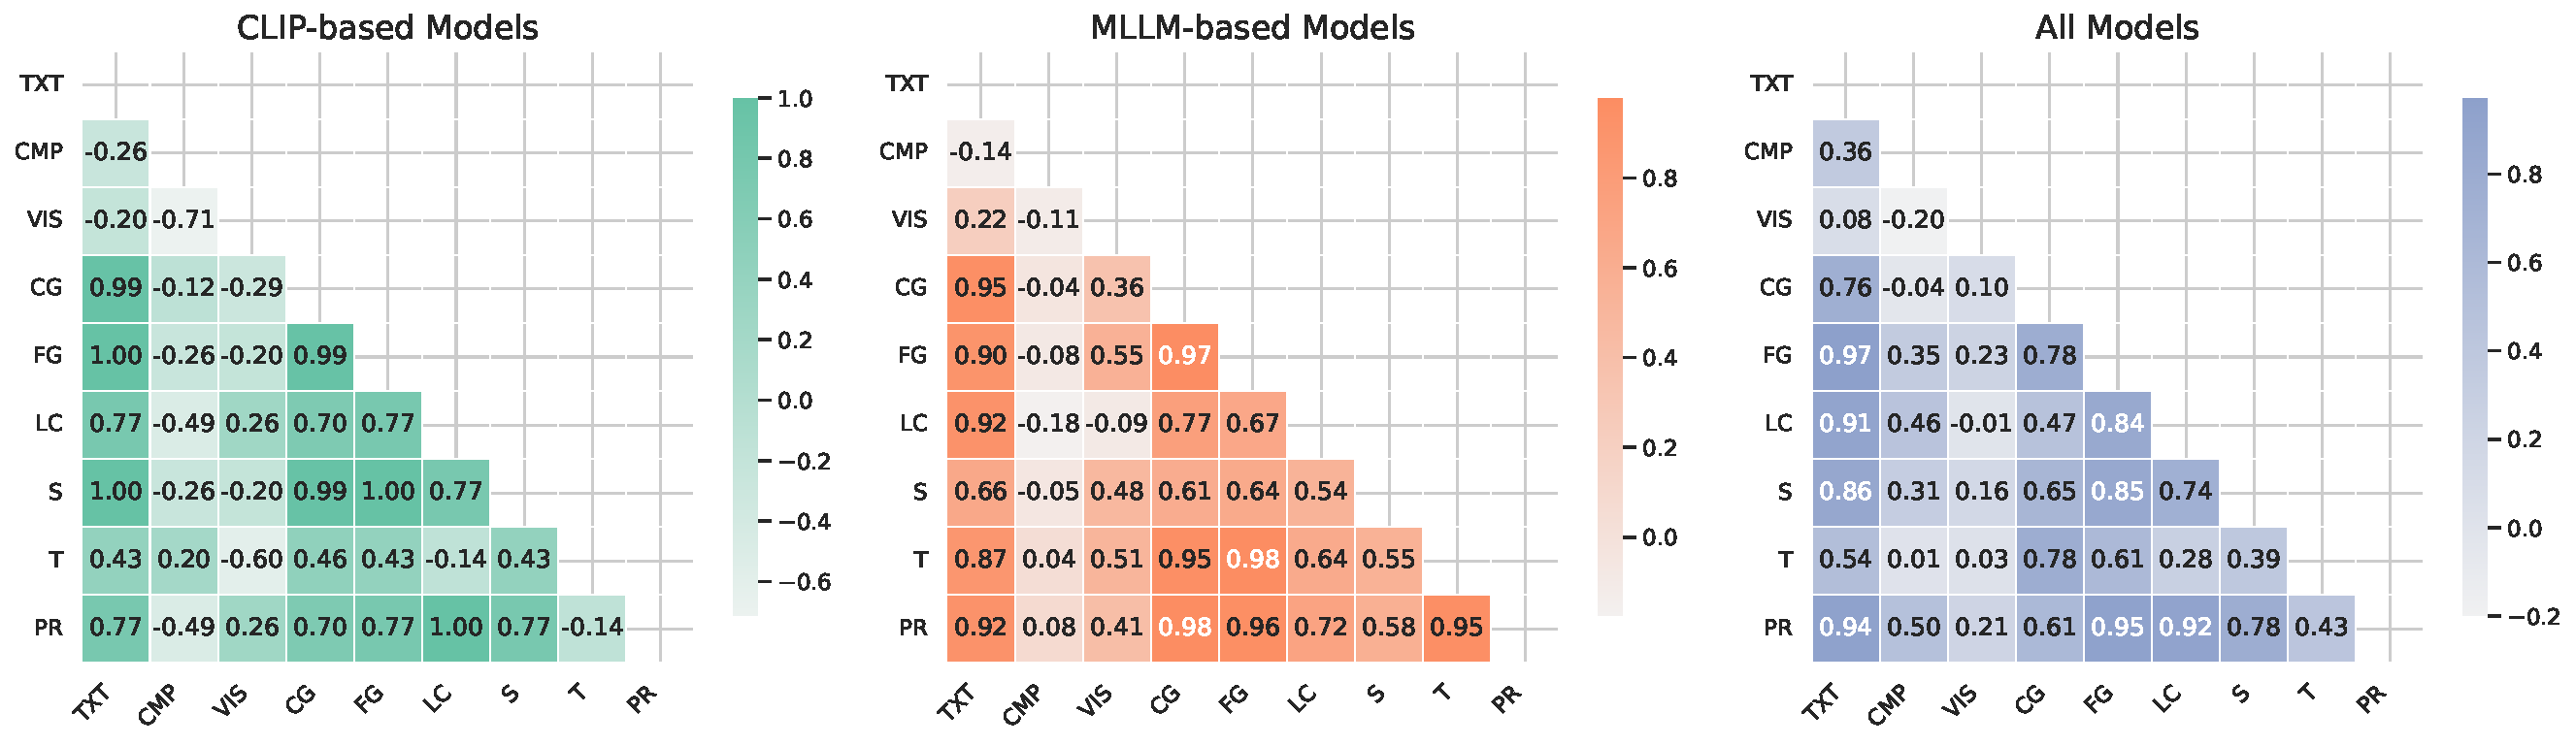
\includegraphics[width=\linewidth]{figures/gve/corr_matrices.pdf}
    \caption{Correlation between dimensional abilities on UVRB for CLIP- and MLLM-based models.}
    \label{gve:fig:corr_ability}
\end{figure}

\begin{figure}[t]
    \centering
    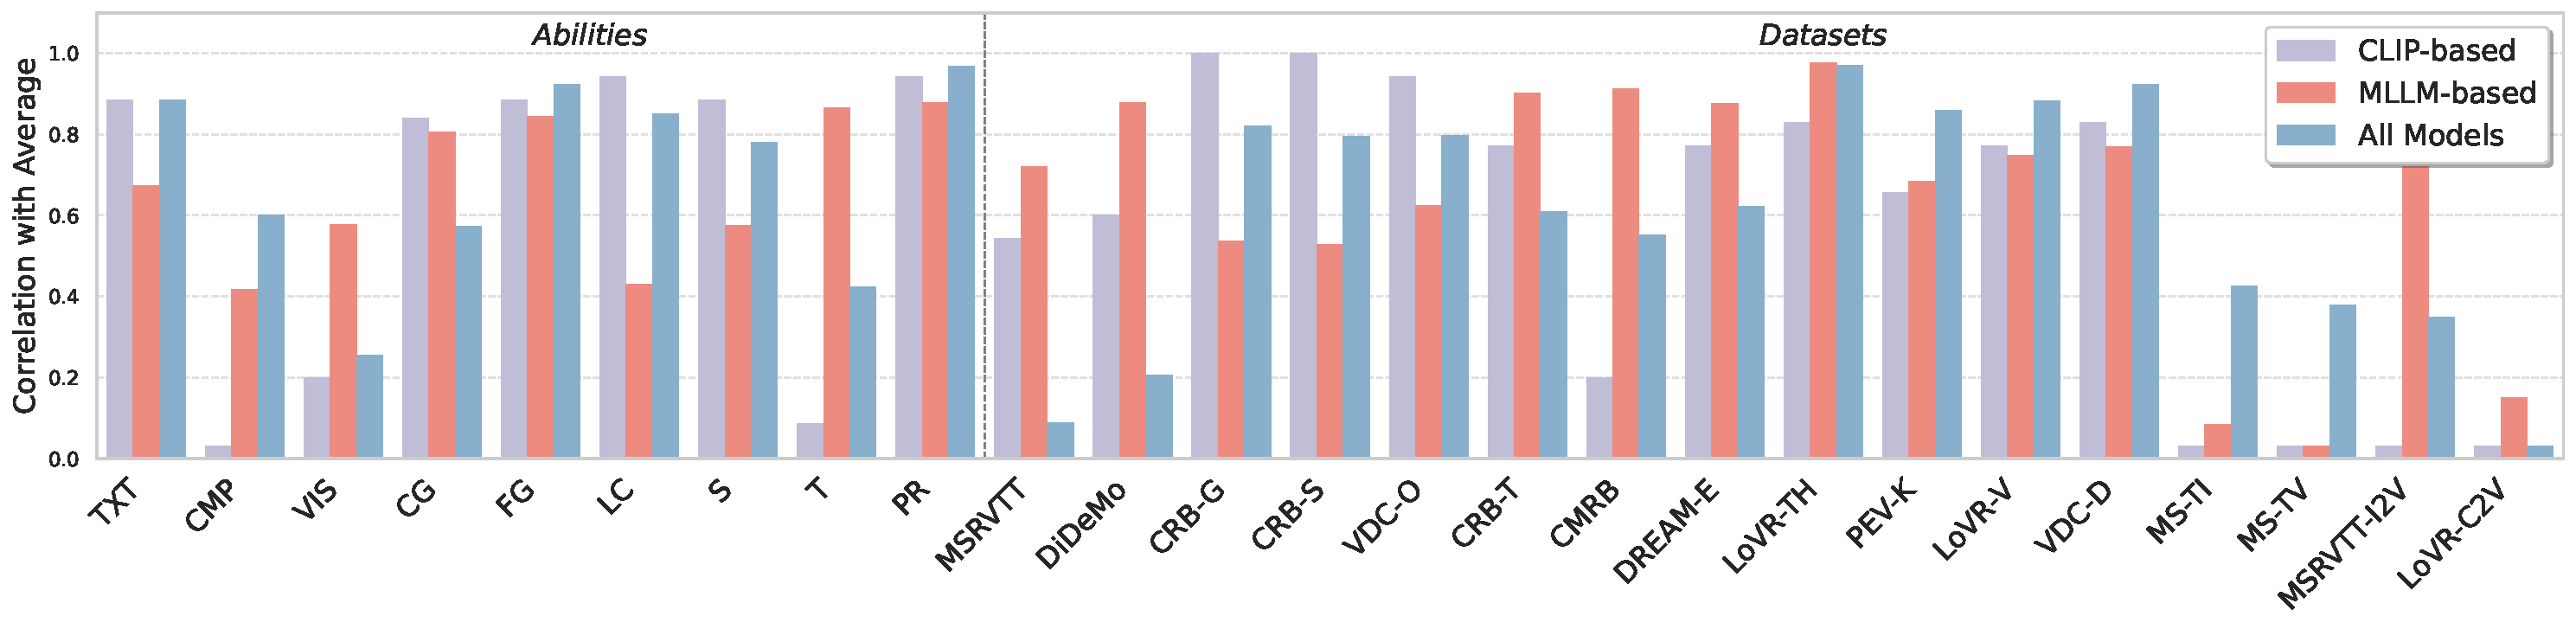
\includegraphics[width=\linewidth]{figures/gve/corr_ability_and_data.pdf}
    \caption{Correlation between averaged performance and individual abilities or datasets on UVRB.}
    \label{gve:fig:corr_task_data}
\end{figure}

\paragraph{Finding 1: Partially Relevant Video Retrieval Better Reflects Universality than Traditional Benchmarks.}
Standard benchmarks such as MSRVTT show a low correlation with average UVR performance ($\rho_{\text{avg}} = 0.58$), suggesting limited representativeness, likely due to overfitting or simplified task design. In contrast, fine-grained (FG), partially relevant (PR), and long-context (LC) retrieval exhibit strong mutual correlations ($\rho \geq 0.90$). More importantly, PR retrieval, although understudied, achieves the highest average correlation with overall performance ($\rho_{\text{avg}} = 0.97$), positioning it as the most reliable proxy for universal capability. We hypothesize this is because successful PR retrieval demands an embedding space that preserves a rich spectrum of information, e.g., from global context to subtle, localized details, rather than collapsing video semantics into a single ``gist''. The ability to maintain this multi-granular semantic richness is a core tenet of universal capability.

\paragraph{Finding 2: Disentangled Spatial and Temporal Representations.}
Models exhibit a marked decoupling between spatial (S) and temporal (T) representation ($\rho = 0.12$). This asymmetry is critical because temporal skills dominate fine-grained understanding ($\rho_{\text{T-FG}} = 0.98$), while spatial skills contribute minimally ($\rho_{\text{S-FG}} = 0.39$). This suggests that current models fail to jointly model \textit{when} and \textit{where}, highlighting the requirements for inductive biases that encourage spatiotemporal integration in video embedding.

\paragraph{Finding 3: Performance Divergence Between CLIP and MLLM-based Models.}
Model failures are architecture-dependent. For example, CLIP-based models are spatially biased ($\rho_{\text{S-CG}} = 0.99$) but temporally weak ($\rho_{\text{T-CG}} = 0.46$), leading to ability trade-offs. Compositional representation inversely correlates with visual accuracy ($\rho_{\text{CMP-VIS}} = -0.71$), and there is a near-zero link between temporal and long-context skills ($\rho_{\text{T-LC}} = -0.14$). In contrast, MLLM-based models demonstrate more balanced and integrated learning: superior semantic matching (PR-CG: MLLM $\rho = 0.98$ vs. CLIP $0.70$) and stronger temporal-long-context coupling ($\rho_{\text{LC-T}} = 0.64$). Therefore, architecture fundamentally shapes the development of capability, and MLLMs have become increasingly popular because of their generalizability in video embedding modeling.

\paragraph{Finding 4: Scaling Has Limited Impact on Visual Perception.}
Parameter scaling improves high-level semantic coherence, but yields negligible gains in low-level visual perception. Notably, the $87$M-parameter \texttt{CLIP4Clip} (VIS: $0.714$) defeats the $8$B-parameter \texttt{Unite-7B} (VIS: $0.702$). Given the weak correlation between visual fidelity and overall retrieval success ($\rho_{\text{AVG-VIS}} = 0.26$), future progress requires targeted improvements in visual grounding.

\FloatBarrier
\subsection{Additional Scaling and Optimization Analyses}

The capability analysis identifies the semantic dimensions that remain difficult. We next examine how training-data scale, inference-time input density, and optimization behavior affect these dimensions. These analyses extend the main comparison by explaining where additional scale helps, where it saturates, and whether the heterogeneous curriculum remains stable during training.


\begin{figure}[t]
    \centering
    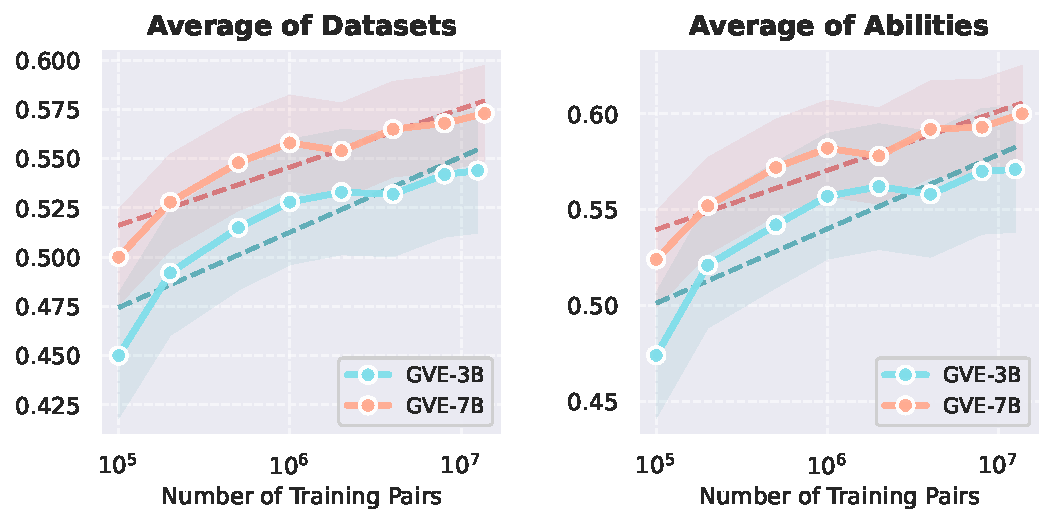
\includegraphics[width=\linewidth]{figures/gve/scaling_avg.pdf}
    \caption{Average performance as a function of training data scale for the GVE series.}
    \label{gve:fig:scaling_avg}
\end{figure}

\subsubsection{Training-Data Scaling}\label{gve:sec:data_scaling}
Figure~\ref{gve:fig:scaling_avg} shows the training-time scaling behavior that performance logarithmically improves with more data, but with diminishing returns.
We quantify scaling efficiency by fitting a logarithmic model $y = a \ln x + b$~($x$: data size, $y$: performance) and report the absolute and relative gain per $10\times$ data increase.
On average across datasets~(abilities), \texttt{GVE-3B} improves by $+7.4\%$~($+7.1\%$) per decade, while \texttt{GVE-7B} gains $+5.4\%$~($+5.4\%$).
While \texttt{GVE-3B} exhibits higher scaling efficiency in relative terms, \texttt{GVE-7B} starts from a higher baseline, suggesting a trade-off between scaling slope and absolute capability.
This result highlights the potential for scaling a more powerful video embedding model with training data at a larger scale.
Figure~\ref{gve:fig:scaling_detail} further decomposes this trend by capability. GVE-3B improves more rapidly on semantic and compositional tasks, including a $14.7\%$ relative gain on CMP and an $11.1\%$ gain on CG per decade of data. GVE-7B shows smaller relative gains on these tasks but benefits more on long-context retrieval, where it improves by $5.4\%$ compared with $3.8\%$ for GVE-3B. This task-dependent pattern suggests that model size affects not only absolute capability but also the scaling profile of different retrieval abilities.

\begin{figure}[t]
    \centering
    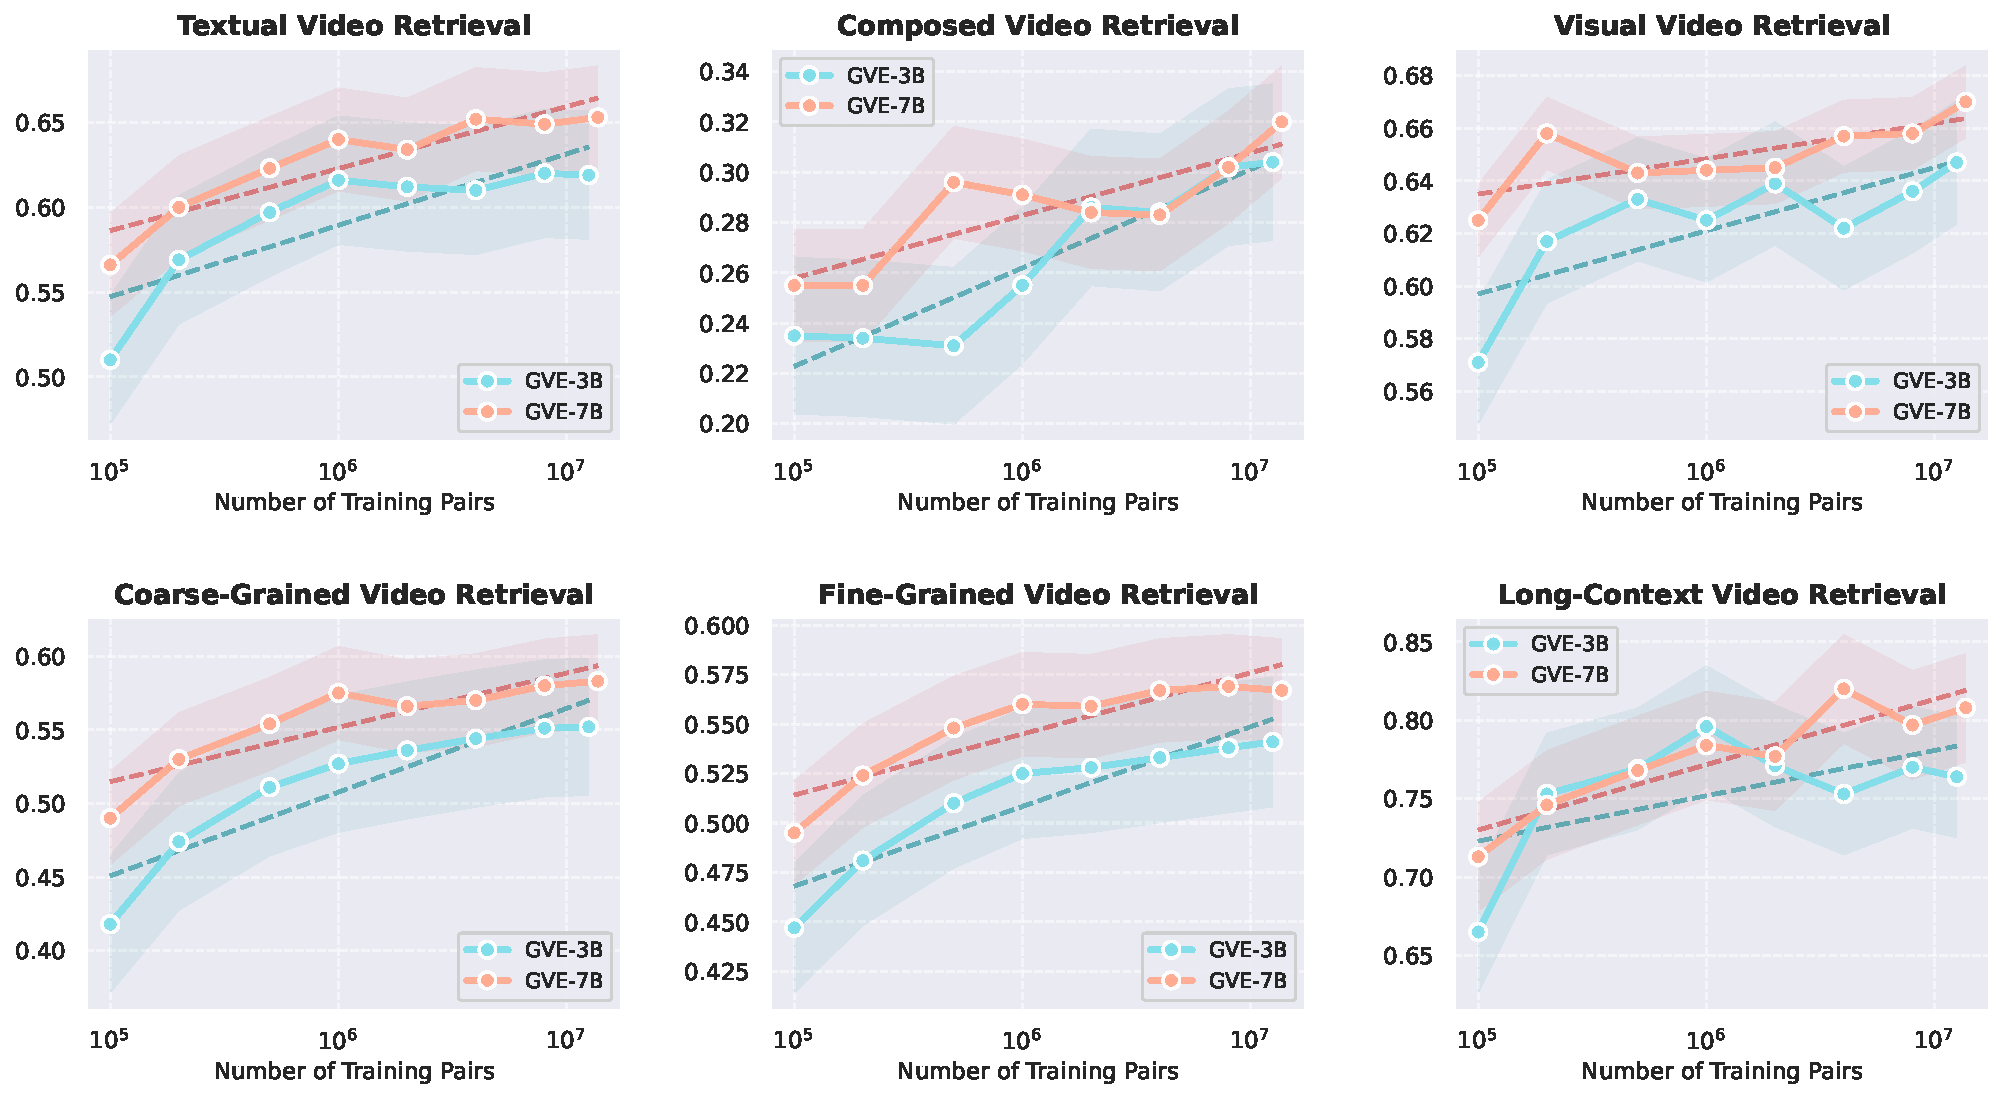
\includegraphics[width=\linewidth]{figures/gve/scaling_detail.pdf}
    \caption{Capability-specific training-data scaling results for GVE-3B and GVE-7B. Shaded bands show $\pm1$ standard deviation, and dashed curves are log-linear fits.}
    \label{gve:fig:scaling_detail}
\end{figure}

\subsubsection{Test-Time Scaling}
We investigate two inference-time parameters for GVE: the number of sampled frames and the maximum number of tokens per frame, which determines the effective spatial resolution. We vary each parameter independently. When the frame count increases from $8$ to $48$, the maximum token count is fixed at $200$. When the token count increases from $200$ to $800$, the frame count is fixed at $8$.

\textit{Temporal scaling.}
As shown in Figure~\ref{gve:fig:scaling_frame}, increasing the number of sampled frames generally improves performance. The largest gains appear in Long-Context retrieval (GVE-3B: $+19.6\%$, GVE-7B: $+12.8\%$), underscoring the value of denser temporal sampling for long-range reasoning. Composed retrieval instead shows a slight degradation, suggesting sensitivity to redundant visual cues from excessive frames. Although GVE-7B consistently outperforms GVE-3B, the average gap across datasets narrows from $0.029$ to $0.024$ as the frame count increases. This indicates that the larger model extracts information more efficiently from sparse inputs.

\textit{Spatial scaling.}
Increasing the token budget yields non-monotonic returns (Figure~\ref{gve:fig:scaling_resolution}). Performance for most tasks peaks around $400$ tokens and then declines. This suggests an optimal level of spatial detail for semantic retrieval. Beyond that point, redundant fine-grained features can dilute the effective semantic signal within the context window. Composed retrieval again deteriorates as the token count increases, reinforcing its sensitivity to input redundancy.

\textit{Implications.}
The results show that temporal scaling provides reliable but diminishing gains, particularly for long-range tasks. Spatial scaling instead exhibits a clear optimum around $400$ tokens, after which additional detail becomes a distraction. The smaller GVE-3B model benefits more from input scaling, whereas GVE-7B shows greater intrinsic efficiency under sparse inputs. These model-specific observations motivate the systematic study of spatiotemporal allocation and density mismatch in Chapter~\ref{ch:spatiotemporal-scaling}.

\begin{figure}[!t]
    \centering
    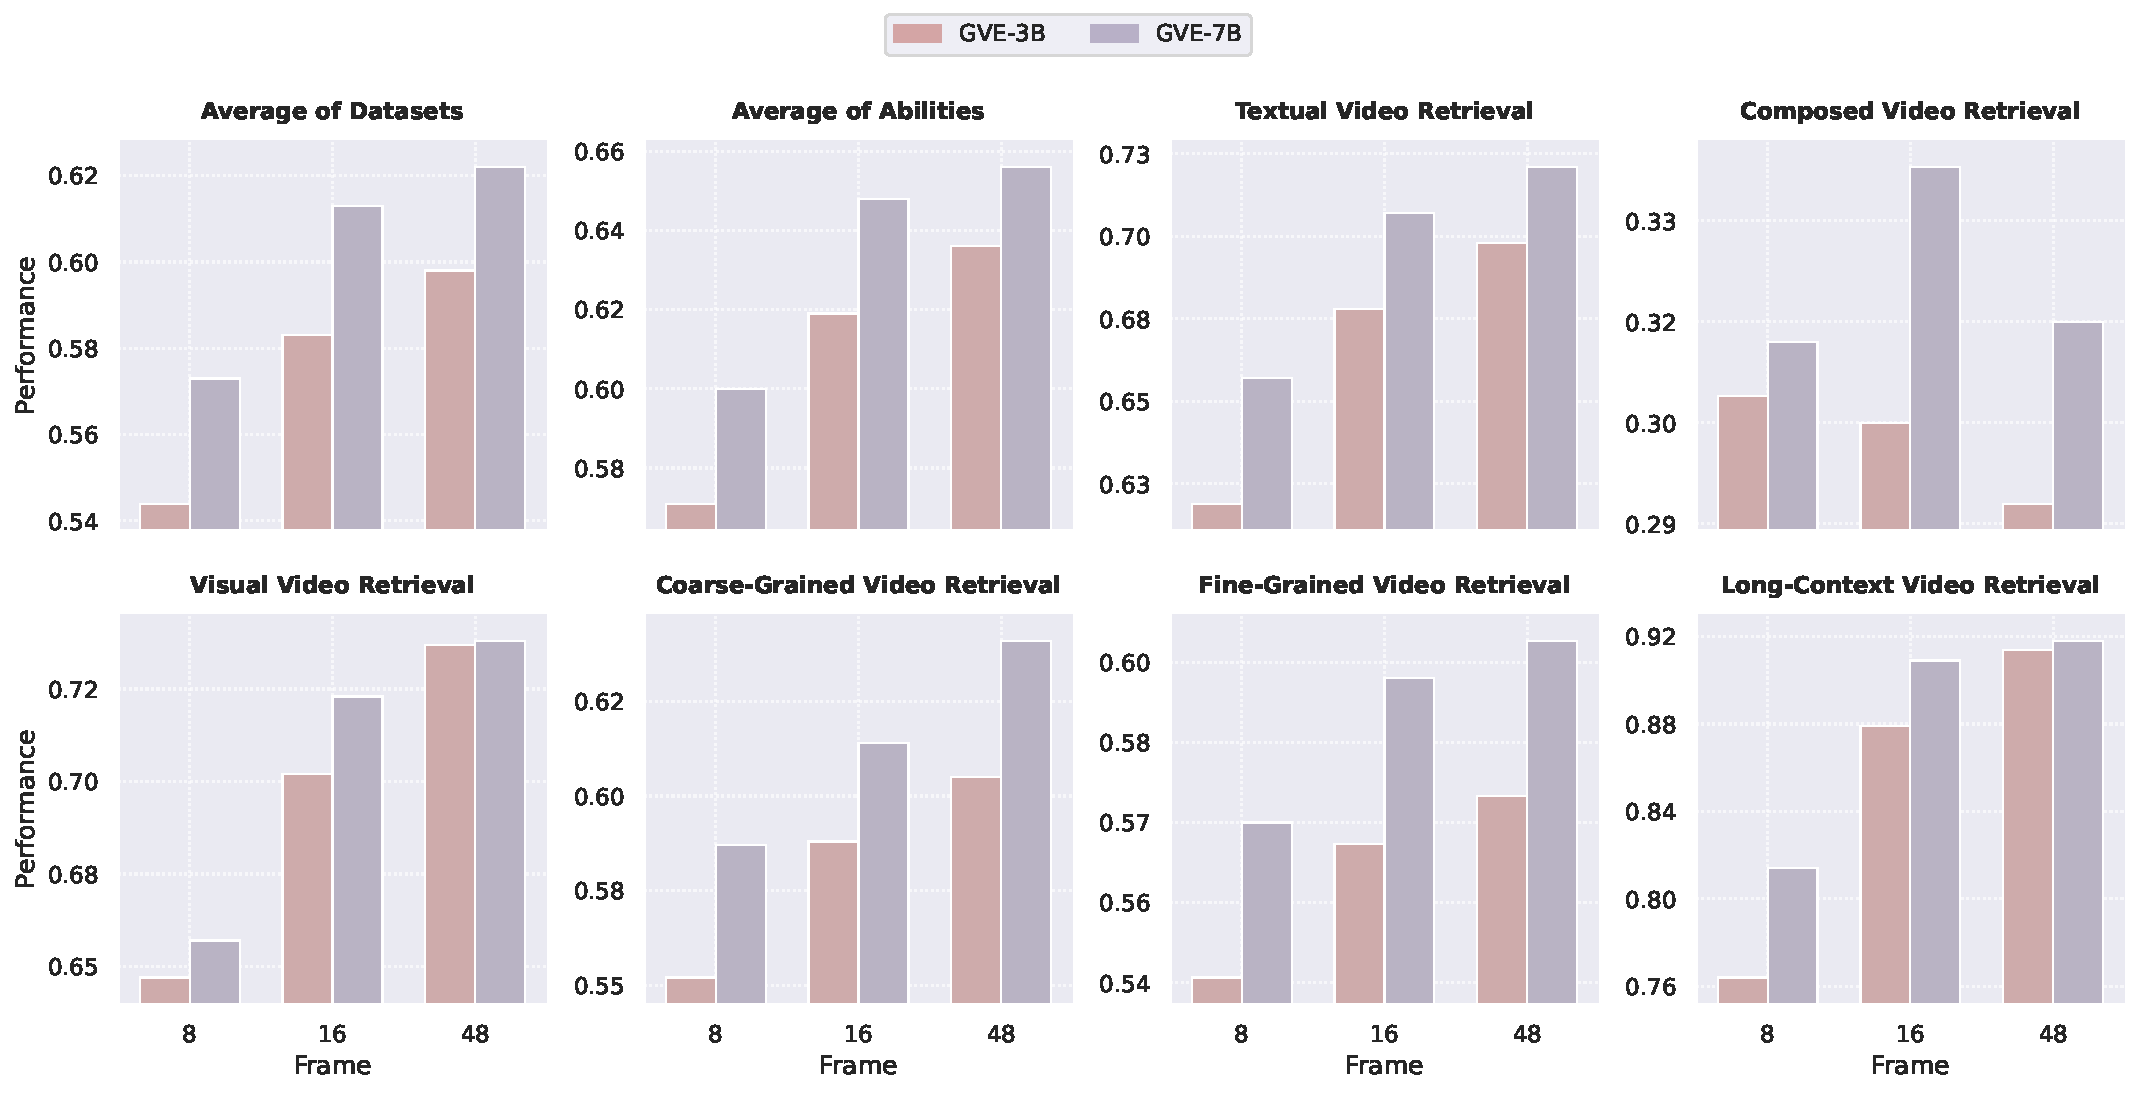
\includegraphics[width=\linewidth]{figures/gve/scaling_frame.pdf}
    \caption{GVE performance as a function of the number of sampled frames at inference time, with the maximum token count fixed at $200$.}
    \label{gve:fig:scaling_frame}

    \vspace{0.5em}
    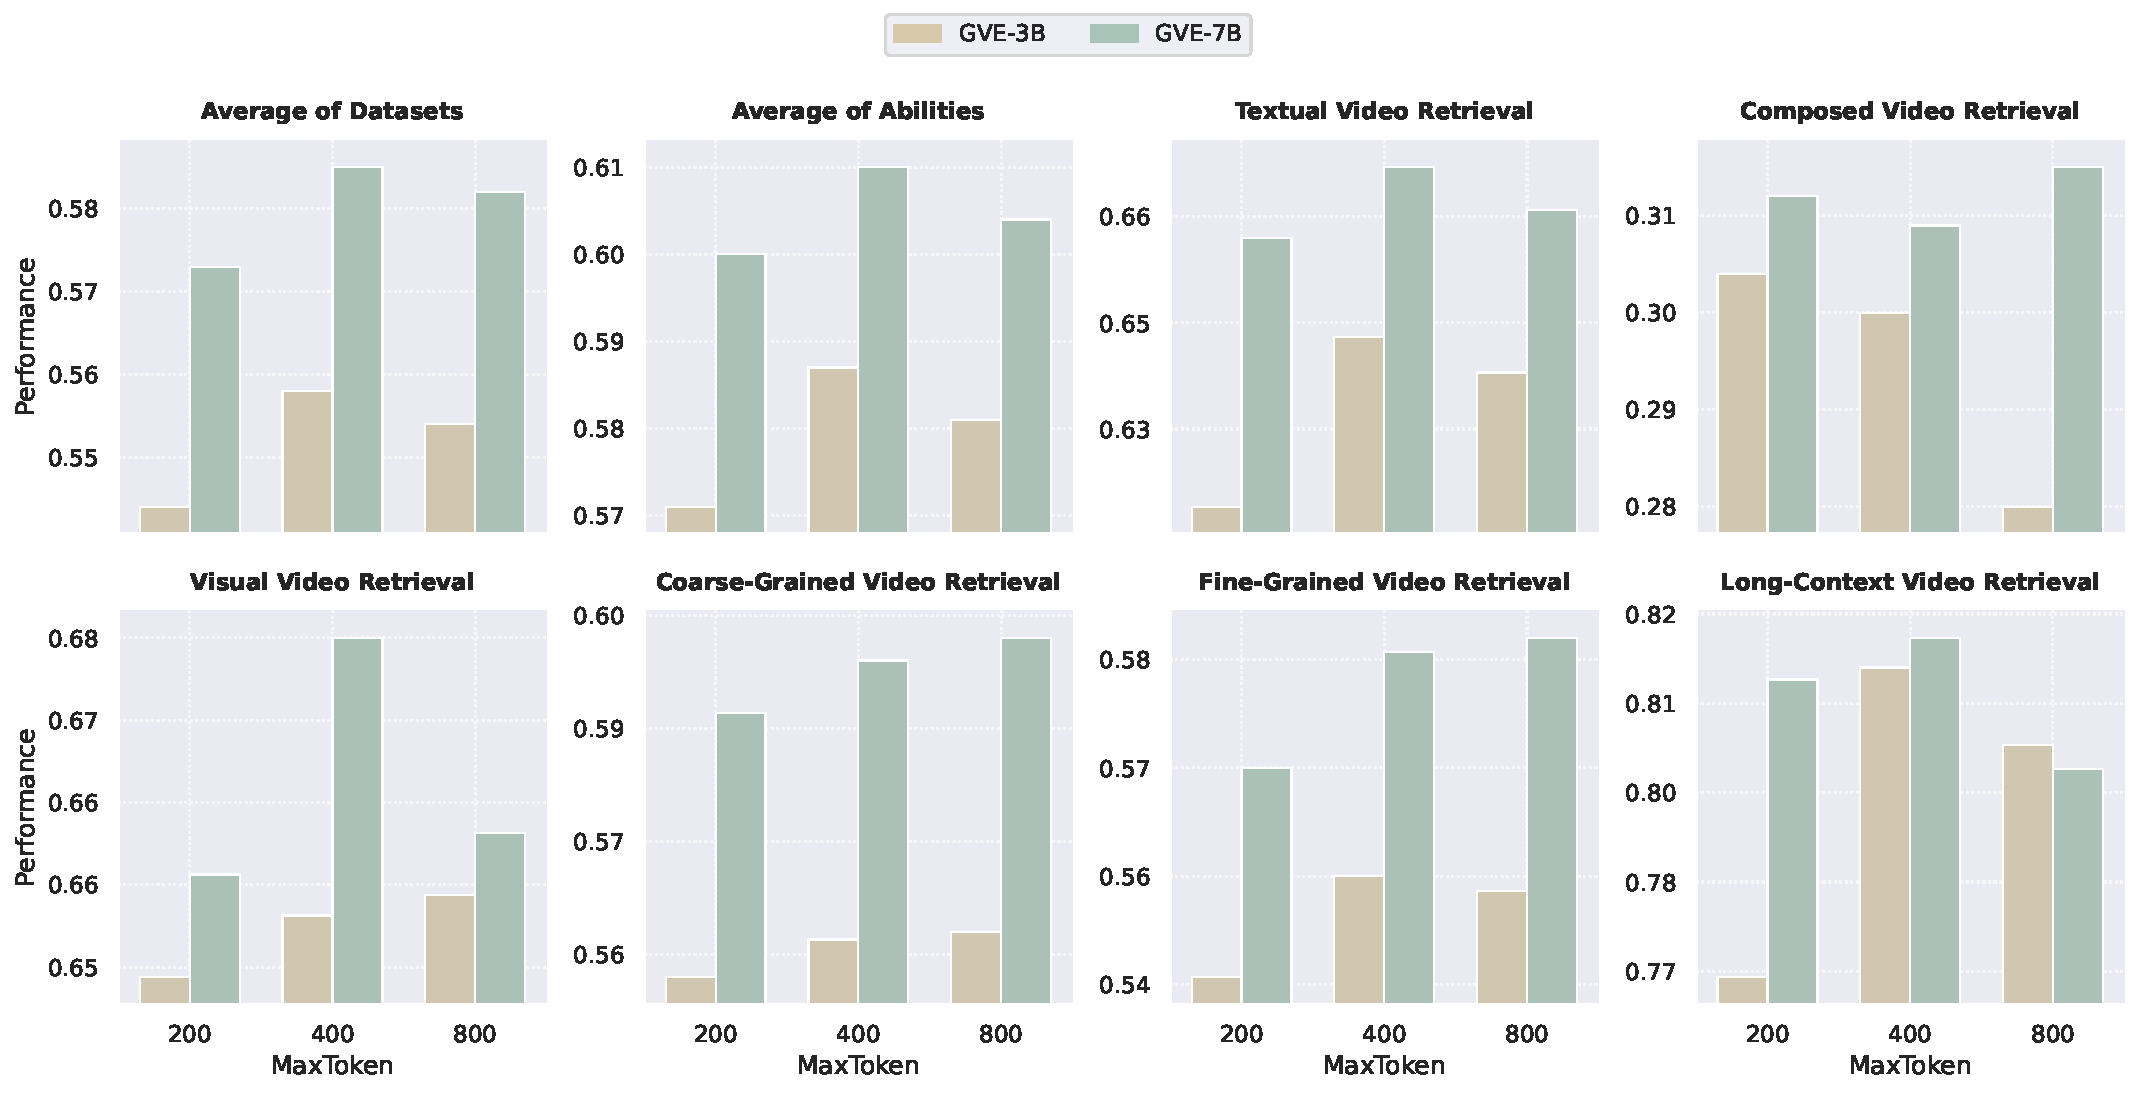
\includegraphics[width=\linewidth]{figures/gve/scaling_resolution.pdf}
    \caption{GVE performance versus the maximum number of tokens per frame, with the frame count fixed at $8$.}
    \label{gve:fig:scaling_resolution}
\end{figure}

\subsubsection{Training Dynamics}
Finally, we inspect optimization stability through four logged quantities: \textit{Training Loss}, \textit{Mean Score}, \textit{Max Negative Gap}, and \textit{Mean Positive Score}. Figure~\ref{gve:fig:training_dynamics} reports the trajectories for GVE-3B and GVE-7B. To reduce the visual influence of isolated outliers, the plots include a $200$-step moving average together with original trajectories subsampled every $100$ steps. Shaded bands indicate $\pm1$ local standard deviation.

\begin{figure}[!t]
    \centering
    \subfloat[GVE-3B.]{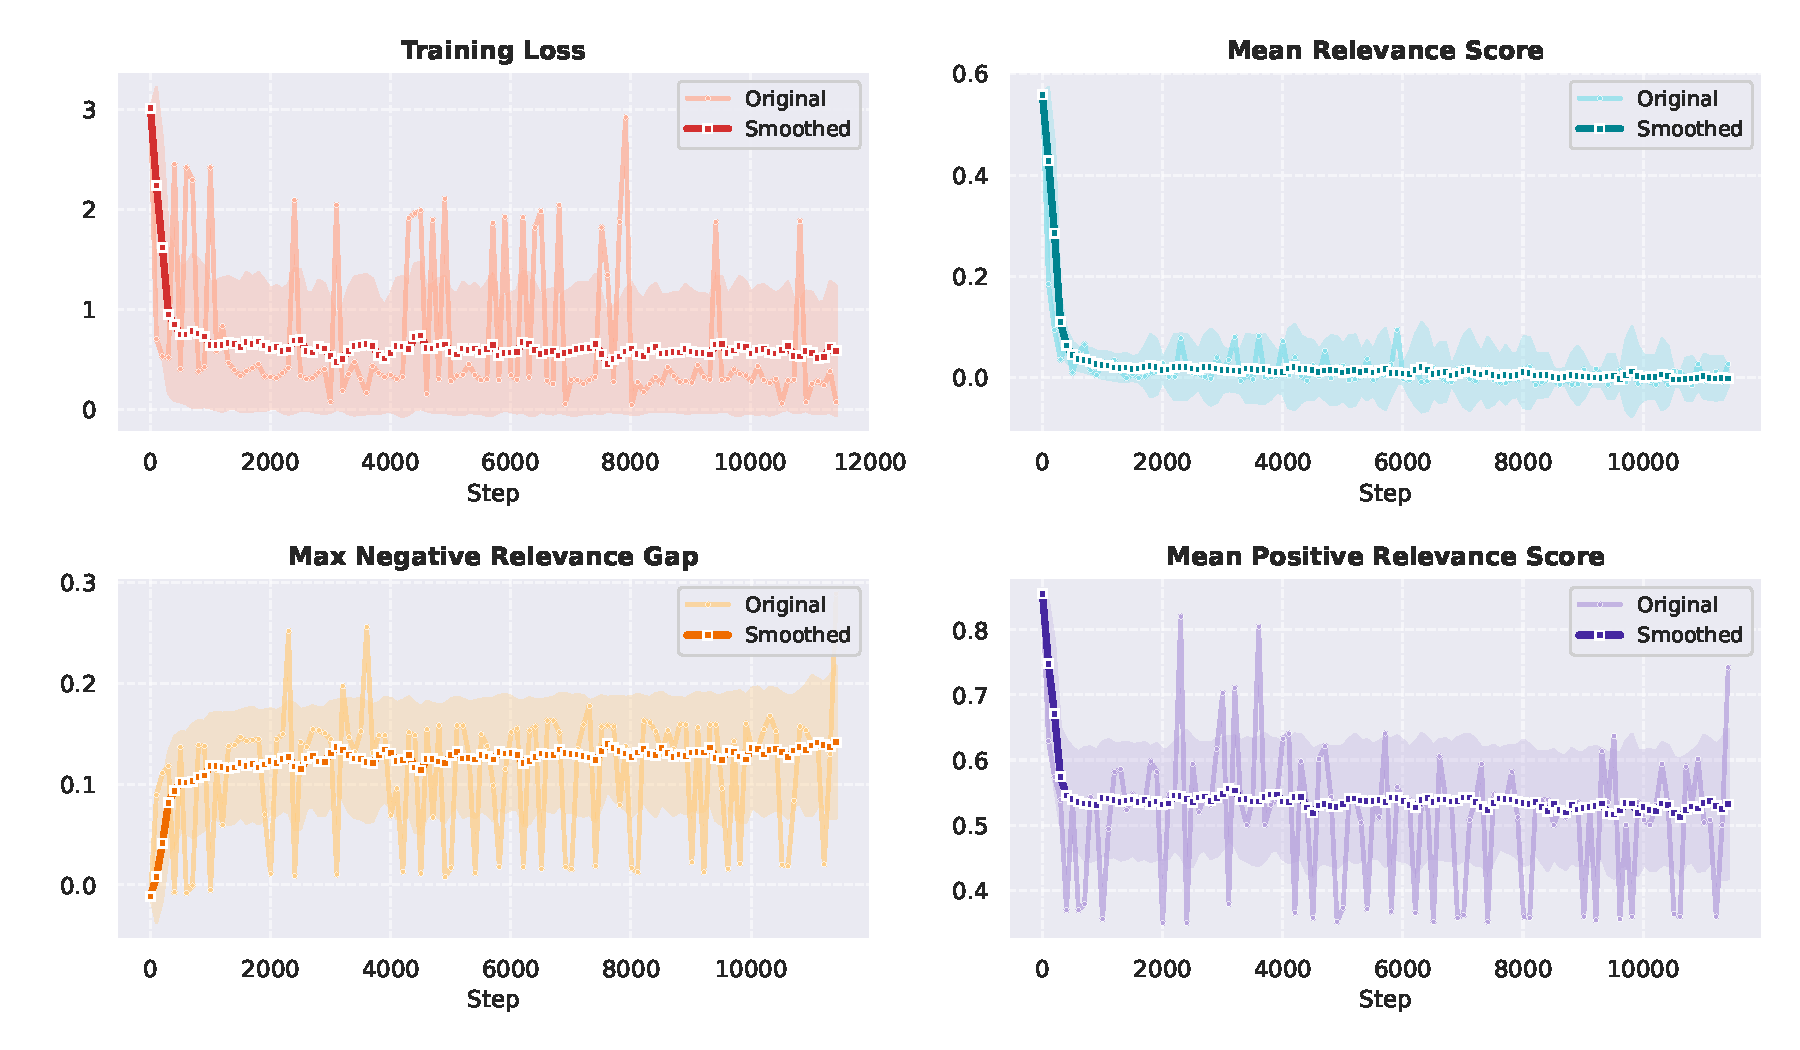
\includegraphics[width=\linewidth]{figures/gve/train_stat-qwen25vl_3b_all_0911.pdf}}\\[-0.5ex]
    \subfloat[GVE-7B.]{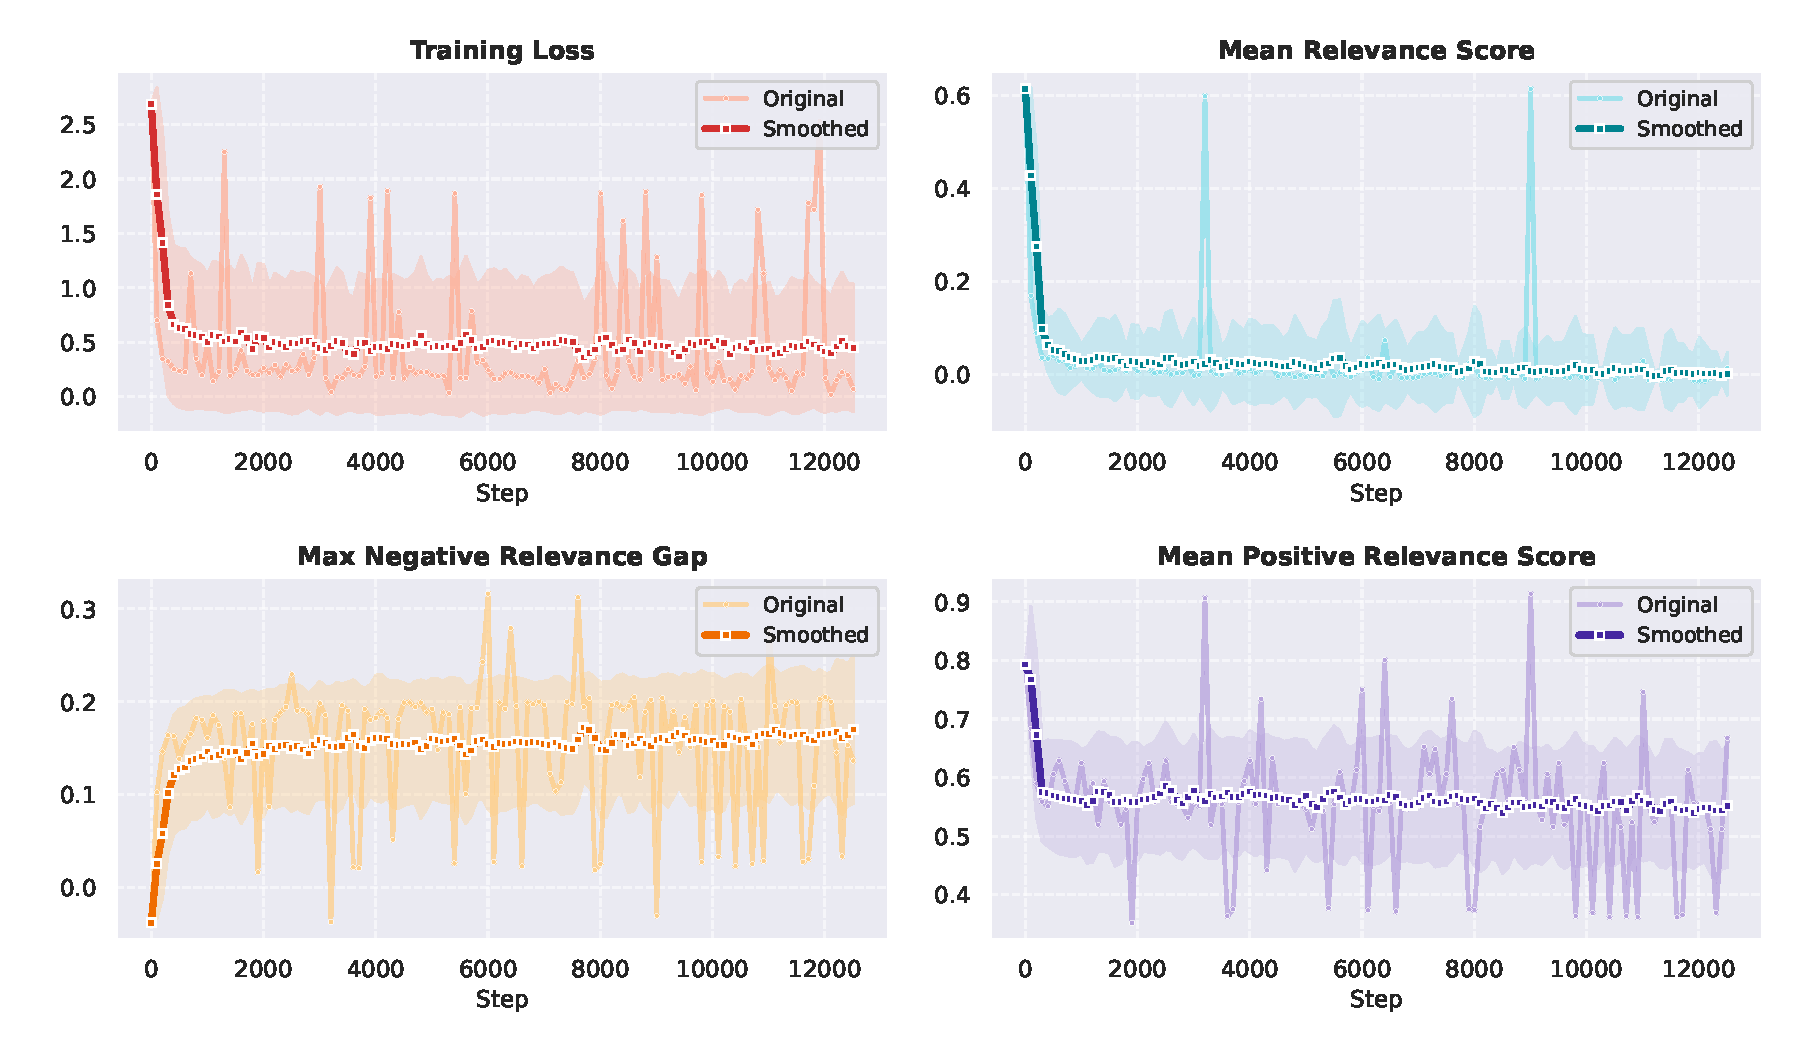
\includegraphics[width=\linewidth]{figures/gve/train_stat-qwen25vl_7b_all_0912.pdf}}
    \caption{Training dynamics of the GVE models across four optimization metrics.}
    \label{gve:fig:training_dynamics}
\end{figure}

\FloatBarrier
\subsection{Zero-Shot Video Classification}

\begingroup\emergencystretch=2em
The preceding experiments evaluate generalization within the UVR capability space. To test whether the learned representation also transfers beyond retrieval, we evaluate GVE on Kinetics-700 (K700)~\cite{carreira2019short}, UCF101~\cite{soomro2012ucf101}, HMDB51~\cite{kuehne2011hmdb}, Something-Something-V2 (SSV2)~\cite{goyal2017something}, and Breakfast~\cite{kuehne2014language}, following MMEB-V2~\cite{meng2025vlm2vec}. Each task is cast as video-to-text retrieval over the complete label set using the standard validation or test split, without training on the target datasets.
\par\endgroup

Table~\ref{gve:tab:video_classification} shows that GVE-7B and InternVideo2-6B attain the highest mean accuracy of $0.526$. GVE-7B also achieves the best UCF101 accuracy and competitive results on the other datasets, indicating that the unified embedding transfers to label-space matching without task-specific adaptation. The lower results on temporally complex datasets such as Breakfast and SSV2 are consistent with the temporal modeling bottleneck identified by the dimensional analysis. The classification results therefore provide an external transfer check while preserving the same zero-shot evaluation principle used throughout the chapter.

\begin{table}[t]
\centering
\caption{Zero-shot video classification accuracy. The highest and second-highest results in each column are bolded and underlined, respectively.}
\label{gve:tab:video_classification}
\begin{tabular}{@{}l|>{\columncolor{gray!15}}c|*{5}{c}@{}}
\toprule
\textbf{Model} & \textbf{AVG} & \textbf{K700} & \textbf{UCF101} & \textbf{HMDB51} & \textbf{SSV2} & \textbf{Breakfast} \\
\midrule
CLIP4Clip       & 0.378 & 0.395 & 0.596 & 0.413 & 0.308 & 0.176 \\
InternVideo2-6B & \textbf{0.526} & \textbf{0.554} & 0.572 & 0.480 & \textbf{0.569} & \textbf{0.453} \\
VLM2Vec-V2      & 0.393 & 0.380 & 0.600 & 0.409 & 0.428 & 0.148 \\
GME-7B          & 0.374 & 0.397 & 0.547 & 0.479 & 0.306 & 0.143 \\
UniME-7B        & 0.306 & 0.388 & 0.377 & 0.407 & 0.190 & 0.166 \\
Unite-7B        & \underline{0.519} & 0.537 & \underline{0.752} & \textbf{0.534} & 0.513 & 0.261 \\
\midrule
GVE-3B          & 0.476 & 0.489 & 0.661 & 0.483 & 0.471 & 0.277 \\
GVE-7B          & \textbf{0.526} & \underline{0.540} & \textbf{0.757} & \underline{0.525} & \underline{0.521} & \underline{0.289} \\
\bottomrule
\end{tabular}
\end{table}

\FloatBarrier
\section{Chapter Summary}

This chapter addressed the semantic-scaling stage of the thesis by asking how one video embedding model can generalize across heterogeneous query formats, domains, and levels of semantic detail. It formulated universal video retrieval and organized 16 public datasets into the UVRB evaluation protocol. The chapter then introduced V-SynFlow and UVRD to supply targeted supervision for underrepresented retrieval capabilities, together with the Modality Pyramid curriculum to stabilize learning across heterogeneous tasks. The main results and ablations showed that both the synthesized data and the curriculum contribute to the performance of GVE under zero-shot evaluation.

The dimensional analysis further showed that conventional benchmarks alone do not adequately represent universal retrieval capability. Partially relevant, fine-grained, and long-context retrieval provide stronger diagnostic signals, while spatial and temporal abilities remain weakly coupled. The scaling, training-dynamics, and video-classification studies clarified how these capabilities respond to additional data, denser inputs, and transfer beyond retrieval. Within the thesis, this chapter establishes broad semantic coverage as the first requirement for scalable video retrieval. It also exposes a remaining limitation: a semantically general representation can only use evidence that is present in its sampled input. This limitation motivates the observational-scaling study in Chapter~\ref{ch:spatiotemporal-scaling}.

\chapter{Observational Scaling for Multi-Granular Long-Video Retrieval}
\label{ch:spatiotemporal-scaling}

\section{Introduction}

Chapter~\ref{ch:universal-video-retrieval} broadens the semantic conditions that a video representation is expected to support. Yet even a generalizable representation remains bounded by the visual evidence supplied to the model. This chapter therefore addresses observational scaling: how faithfully an embedding preserves the evidence required by queries at different temporal granularities under constrained sampling.

Real-world videos are increasingly long and informationally dense, spanning tens of minutes to hours~\cite{henschel2025streamingt2v,weng2024longvlm}, while a query may describe anything from the overall theme to a brief moment~\cite{xiao2022video,chen2023joint}. Since encoding every frame at full resolution is computationally prohibitive~\cite{hu2022mmsampler}, spatiotemporal sampling determines which evidence is available to the representation~\cite{guo2025gve}. Too few frames or too low a resolution can cause the target moment to be missed entirely. Although previous work has demonstrated sensitivity to sampling~\cite{guo2025gve,zhu2025dynamic}, its interaction with query granularity remains underexplored because no existing benchmark provides a multi-granular and controllable testbed. The relevant benchmark and embedding literature is reviewed centrally in \S\ref{sec:lr-benchmarks} and \S\ref{sec:lr-embedding}.

\begin{figure}[t]
    \centering
    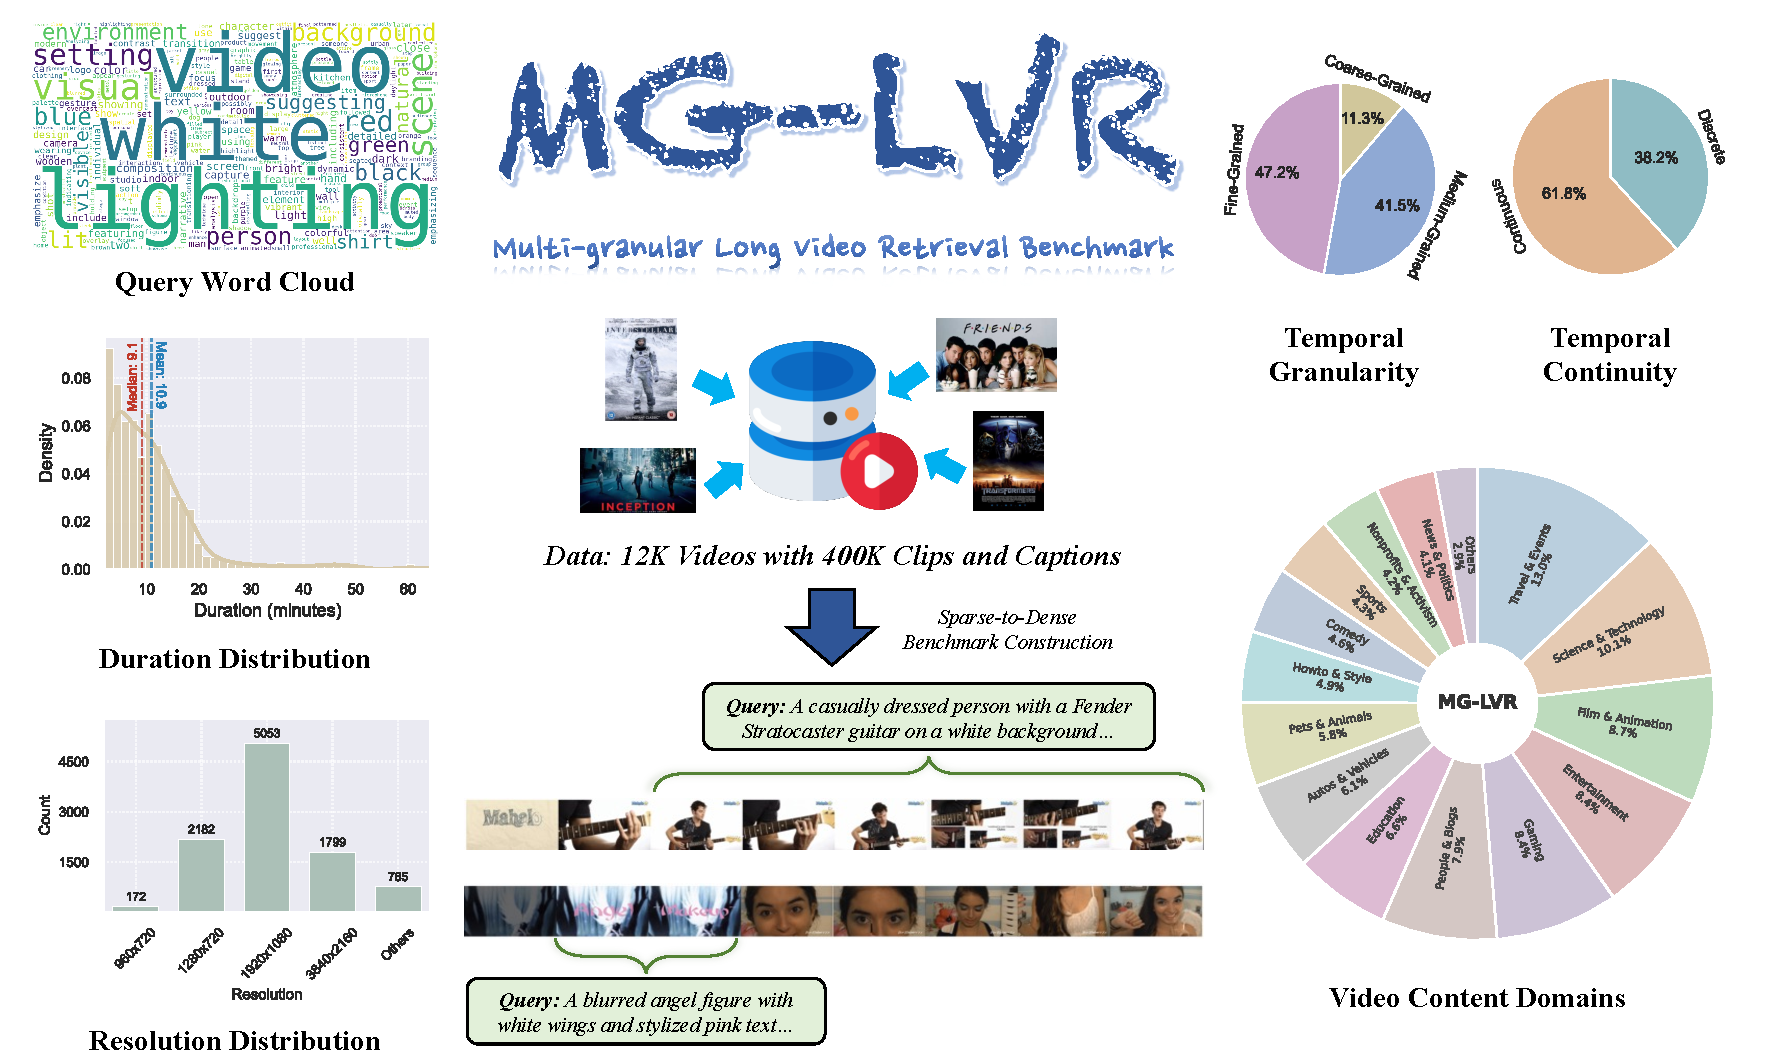
\includegraphics[width=\linewidth]{figures/mglvr/statistics.pdf}
    \caption{Overview of Multi-granular Long Video Retrieval (MG-LVR) benchmark.}
    \label{mglvr:fig:statistics}
\end{figure}

Current benchmarks are insufficient for this purpose. Short-clip datasets such as MSR-VTT~\cite{xu2016msr} and DiDeMo~\cite{anne2017localizing} are too brief for sampling density to have a meaningful impact. Recent long-video retrieval benchmarks~\cite{cai2025lovr} extend the temporal scope but evaluate at a single query granularity, making it impossible to determine whether sampling configurations should vary with query specificity. No existing setting jointly provides long-form videos and multi-granular query categorization within a unified evaluation framework. Such a combination is essential for exploring spatiotemporal scalability across diverse semantic scales.

To address this gap, we introduce the Multi-Granular Long Video Retrieval (\benchmarkname) benchmark shown in Figure~\ref{mglvr:fig:statistics}. \benchmarkname pairs long-form videos with queries categorized by temporal granularity, defined as the fraction of the video duration that a query covers. Importantly, the benchmark allows the relevant evidence for a query to be grounded either in a single clip or across multiple clips that may occur at different timestamps, reflecting realistic retrieval scenarios. Evaluation across 23 models reveals a pronounced granularity gap: fine-grained retrieval lags coarse-grained performance by over 75\% under sparse sampling and recovers only marginally as frame count increases. This provides a clear signal for studying how sampling configurations affect retrieval performance across different semantic granularities.

Using \benchmarkname, we conduct a comprehensive spatiotemporal scaling analysis across both Contrastive Language-Image Pretraining (CLIP)-based~\cite{gorti2022x} and Multimodal Large Language Model (MLLM)-based families~\cite{kong2025modality}. At test time, increasing spatial resolution helps most when frames are few, while its benefit saturates at higher frame counts. Under a fixed token budget, the optimal spatial-temporal allocation shifts with query granularity. Coarse queries favor fewer frames at higher resolution, while fine-grained queries favor more frames at lower resolution. At training time, the interaction between spatial and temporal density is asymmetric. Spatial representations are resolution-robust, maintaining accuracy across varying input resolutions. Temporal representations exhibit frame-count anchoring, where performance peaks when the inference frame count matches the training configuration and degrades significantly when they diverge, particularly for fine-grained queries.

This analysis highlights a key insight: the knowledge required for effective low-density inference is already latent within high-density models, but it does not automatically transfer when the sampling configuration changes. To address this, we propose Video Embedding Waterfall (VEterfall), a progressive dense-to-sparse self-distillation framework. Inspired by the waterfall effect, our method cascades high-fidelity semantic knowledge from densely sampled embeddings down to sparser representations. In this way, VEterfall achieves up to a 20\% relative recall gain on fine-grained queries while operating in a 4$\times$ to 16$\times$ more efficient inference setting. Our experiments confirm that the scaling behaviors identified by \benchmarkname can be directly and effectively exploited in practice.

The contributions of this chapter are summarized as follows.
(1)~We introduce \benchmarkname, the first benchmark for multi-granular long-video retrieval that enables scalable research into spatiotemporal sampling.
(2)~We conduct a multi-dimensional scaling analysis that identifies key principles such as frame-count anchoring and granularity-dependent token allocation.
(3)~We propose VEterfall, a self-distillation method that enhances video embeddings under sparse sampling by unlocking multi-granular knowledge already latent within the models.


\begin{table}[t]
    \centering
    \caption{Comparison of text-video retrieval benchmarks. \textbf{MG-LVR} is the first benchmark supporting multi-granular queries for retrieving long-form videos. \textbf{Gran.}: Temporal granularity of queries, including fine~(FN), medium~(MD), and coarse~(CR) -grained; \textbf{Cont.}: Temporal continuity of queries, including discrete~(DC) and continuous~(CT).}
    \label{mglvr:tab:benchmark_comparison}
    \setlength{\tabcolsep}{2.5pt}
    \begin{tabular}{@{}l*{6}{c}@{}}
    \toprule
    \textbf{Dataset} & \textbf{\#~Query} & \textbf{\#~Corpus} & \textbf{Dur~(s)} & \textbf{\#~Word} & \textbf{Gran.} & \textbf{Cont.} \\
    \midrule
    MSRVTT~\cite{xu2016msr} & 1,000 & 1,000 & 15.0 & 9.4 & CR & CT \\
    DiDeMo~\cite{anne2017localizing} & 1,004 & 1,004 & 53.9 & 29.1 & CR & CT \\
    TVR~\cite{lei2020tvr} & 10,895 & 2,179 & 76.2 & 13.4 & FN, MD & CT \\
    ActivityNet Captions~\cite{krishna2017dense} & 18,000 & 4,917 & 117.6 & 14.8 & FN, MD & CT \\
    LoVR~\cite{cai2025lovr} & 100 & 467 & 1560.3 & 17364.5 & CR & CT \\
    VDC~\cite{chai2024auroracap} & 1,000 & 1,027 & 30.1 & 508.0 & CR & CT \\
    \midrule
    \textbf{MG-LVR (Ours)} & 9,971 & 4,844 & 705.9 & 44.7 & All & Both \\
    \bottomrule
    \end{tabular}
\end{table}

\section{Rethinking Text-Video Retrieval Evaluation}
\label{mglvr:sec:benchmark}

Text-video retrieval has historically been formulated as a global-matching task, where each query describes the entirety of its paired video. This convention reflects the structural limitations of existing benchmarks: queries are either brief summaries of short clips or document-level aggregations of dense captions, making the query and video co-extensive by construction and effectively sidestepping the challenge of temporal scale. In the era of long, multi-scene video, this paradigm is insufficient. User intent may range from identifying a moment of a few seconds within an hour-long lecture to capturing the overarching theme of an entire documentary, imposing qualitatively different demands on spatiotemporal sampling and representation density.

As shown in Figure~\ref{mglvr:fig:statistics}, the \textbf{Multi-Granular Long Video Retrieval (MG-LVR)} benchmark is designed to bridge this gap by formalizing \textit{temporal granularity} as an explicit evaluation axis. Unlike traditional datasets~\cite{lei2020tvr,krishna2017dense} where granularity emerges as a byproduct of annotator bias and video readability~(e.g., length, dynamics, complexity), \benchmarkname employs an automated pipeline that explicitly controls query granularity by analyzing semantic relationships among clips within each video, enabling a systematic study of how models navigate the spectrum from localized events to global narratives. The resulting benchmark contains $9,971$ queries paired with a corpus of $4,844$ videos averaging $705.9$ seconds in duration. As summarized in Table~\ref{mglvr:tab:benchmark_comparison}, \benchmarkname is the only benchmark that jointly covers all three granularity levels while supporting both single-clip and multi-clip evidence structures. The dataset and code of MG-LVR will be publicly released upon acceptance. This section first formalizes the evaluation setting, then describes the construction pipeline, and concludes with the complete prompt specifications used for query and caption synthesis.

\subsection{Formulations}
\label{mglvr:sec:formulation}

This chapter retains the query $q$, corpus $\mathcal{V}$, and ranking objective from the unified formulation in \S\ref{sec:bc-vr}. It specializes that formulation to text queries over long-form videos and introduces temporal granularity as an observational variable rather than a different retrieval objective.

Accordingly, the target is $v^{*} = \arg\max_{v \in \mathcal{V}} s(q,v)$. The query may refer to any portion of the video, from a brief localized event to the overall theme, with the fraction of relevant content serving as a variable difficulty factor.

\begin{definition}[\textbf{Temporal Granularity}]
Temporal granularity $G$ is defined as the ratio of relevant content duration to total video length:
\begin{equation}
    G = \frac{|\mathcal{S}(v^{*},\,q)|}{d_{\mathrm{video}}} \in (0,\,1].
    \label{mglvr:eq:granularity}
\end{equation}
As $G \to 0$, retrieval approaches a needle-in-a-video problem in which the target moment occupies a vanishingly small fraction of the video. For systematic evaluation, we partition the granularity spectrum into three categories: \textbf{Fine-grained (FN)}, \textbf{Medium-grained (MD)}, and \textbf{Coarse-grained (CR)}.
\end{definition}

In this work, granularity thresholds are set to $G \in [0.001, 0.01]$ for FN and $G \in [0.1, 0.3]$ for MD, ensuring high inter-class distinctiveness and enabling clear observation of how model performance scales with task difficulty.

For the temporal distribution of relevant content, we further define temporal continuity $C$ to characterize the structural complexity of each retrieval target:
\begin{equation}
    C = \frac{\sum_{i=1}^{k}(e_i - s_i)}{e_k - s_1} \in (0,\,1],
    \label{mglvr:eq:continuity}
\end{equation}
where $[s_i, e_i]$ are the $k$ disjoint intervals composing $\mathcal{S}$. A value of $C=1$ indicates a single contiguous event, while $C<1$ represents fragmented content distributed across multiple disjoint segments, such as a recurring theme.

\begin{figure}[t]
    \centering
    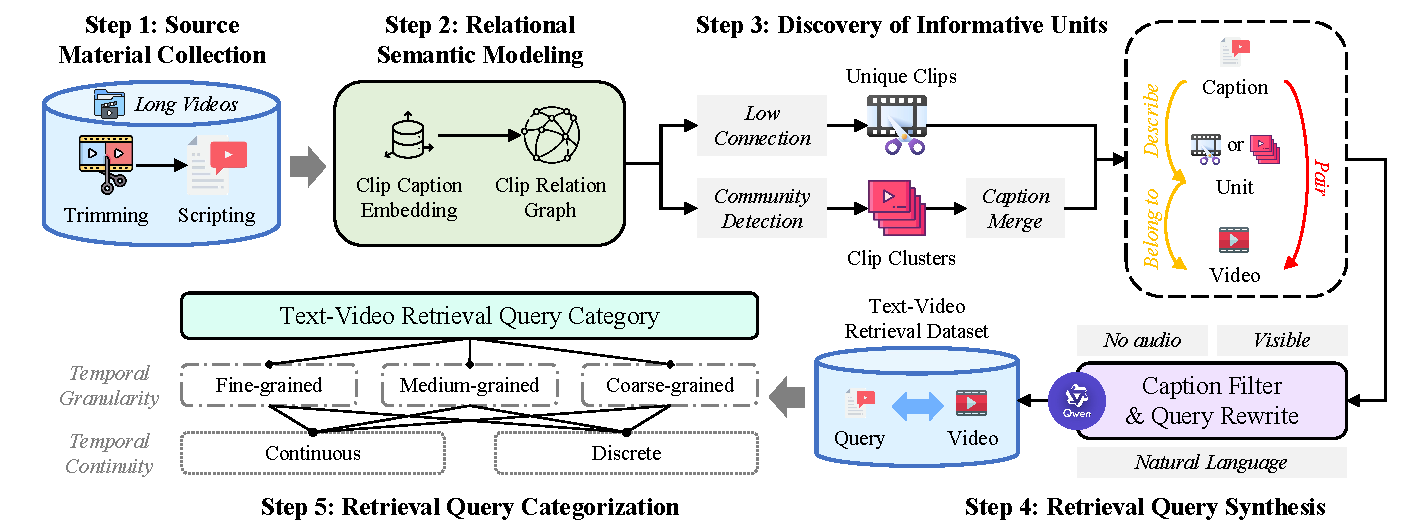
\includegraphics[width=\linewidth]{figures/mglvr/mg-lvr.pdf}
    \caption{The \benchmarkname construction pipeline. We model long videos as \textit{Clip Relation Graphs} to transform unstructured content into a quantifiable semantic topology. This structural foundation allows for the systematic discovery of retrieval units across varying temporal granularities and continuity levels, which are then synthesized by an LLM into natural language queries.}
    \label{mglvr:fig:mg-lvr}
\end{figure}

\subsection{MG-LVR: Sparse-to-Dense Benchmark Construction}
\label{mglvr:sec:construction}

As summarized in Figure~\ref{mglvr:fig:mg-lvr}, we construct \benchmarkname through a semantics-aware pipeline that formalizes video retrieval as a sampling task over structured semantic relationships among clips. The core insight is to represent each video as a similarity graph, enabling the identification of retrieval units that vary in temporal granularity and evidence composition. This approach ensures that \benchmarkname covers scenarios where relevant evidence is grounded either in a single clip or across multiple clips that may occur at different timestamps.

\paragraph{Step 1: Material Curation.}
We build upon the Vript dataset~\cite{yang2024vript}, selecting long videos ($>120$s) with dense, high-quality GPT-4V clip-level captions. These captions serve as semantic proxies, allowing the pipeline to model video content without the prohibitive cost of pixel-level processing during construction.

\paragraph{Step 2: Semantic Topology Modeling.}
To provide a structural basis for unit extraction, each video is represented as a \textit{Clip Relation Graph}, where nodes correspond to clips, and edges correspond to the cosine similarity values between two clip caption embeddings produced by Qwen3-Embedding-8B~\cite{qwen3embedding}. This graph captures semantic relationships among clips: clusters of highly connected nodes often correspond to dominant themes, while weaker connections may indicate localized or transient events.

\paragraph{Step 3: Discovery of Informative Units.}
Retrieval units are extracted from the clip relation graph by applying structural constraints that correspond to our granularity and evidence composition settings. This graph-based discovery allows the benchmark to include both single-clip evidence and semantically related clips that appear at different timestamps.
\textit{Single-Clip Units:} Individual nodes with nearly zero external connections are selected as standalone retrieval units, yielding $32,984$ units.
\textit{Multi-Clip Units:} Identified via Louvain community detection to capture thematically consistent clips that may be dispersed across the timeline, yielding $7,764$ units.

\paragraph{Step 4: Retrieval Query Synthesis.}
An LLM (Qwen3-32B~\cite{yang2025qwen3}) synthesizes the metadata of each unit into a natural language query. For multi-clip units, the model is prompted to generate a holistic description covering the relationships among multiple relevant clips. A subsequent refinement pass filters out ambiguous descriptions and removes references to audio content to ensure a focus on visual information.

\paragraph{Step 5: Retrieval Query Categorization.}
Each query-video pair is assigned to a granularity level (FN, MD, or CR) based on the computed value of $G$. The final benchmark retains $9,971$ queries in total, comprising $4,706$, $4,142$, and $1,123$ queries for FN, MD, and CR, respectively.

\paragraph{Human Validation.}
To ensure retrieval uniqueness, a cross-modal collision check is applied: queries exhibiting high semantic similarity to non-target clips within the same video are pruned. Human validation confirms a $96\%$ accuracy rate over $50$ query-video pairs.


\subsection{Prompt Specifications for MG-LVR Construction}
\label{mglvr:sec:prompt_specs}
% ============================================================

Step~4 of the MG-LVR construction pipeline uses two LLM prompts: one generates retrieval queries from clip-level captions (\S\ref{mglvr:sec:prompt_query}), and the other synthesizes a consolidated visual description of each video (\S\ref{mglvr:sec:prompt_caption}). Both prompts were executed with Qwen3-32B.

\subsubsection{Retrieval Query Synthesis}
\label{mglvr:sec:prompt_query}

This prompt is used in Step~4. It receives the aggregated captions of a retrieval unit together with its granularity $G$ and continuity $C$ values, and produces three natural-language queries of increasing descriptive depth.

\begin{promptbox}{Retrieval Query Synthesis from Captions}
\begin{lstlisting}[style=promptstyle]
## ROLE
You are an expert Search Query Synthesizer. Your primary goal is to read a descriptive video caption and generate three high-quality, divergent search queries that are strictly grounded in the visual information provided.

## CRITICAL RULES & PROCESSING LOGIC

### 1. Core Mandate: Grounded and Diverse Queries
- **Strictly Visual & Factual**: All generated queries, regardless of their complexity, MUST be derived solely from the visual information described in the "Raw Caption". Do not invent details not present (e.g., specific brand names unless visible, people's names unless specified as visual text). Explicitly ignore any mention of audio, speech, voice-overs, sound effects, or metadata. Queries must be declarative sentences, not questions or commands.
- **Three Distinct Perspectives**: For each valid caption, generate exactly three queries. These queries must be genuinely different, reflecting diverse user intents and levels of detail.
  - **Query 1 (Librarian/Factual)**: A concise, objective summary of the core visual elements. Length: 20-50 words.
  - **Query 2 (Everyday User/Descriptive)**: A more narrative and descriptive query, using richer vocabulary to describe the scene, actions, and atmosphere. Length: 30-100 words.
  - **Query 3 (Researcher/Analytical)**: A detailed, analytical query that examines visual composition, spatial-temporal details, potential technical aspects, or the narrative storytelling of the scene. Length: 70-200 words.

### 2. Content Quality Filter: Identify and Discard Invalid Inputs
- Before generating queries, you MUST first assess the "Raw Caption" against the following filters. If a caption falls into any of these categories, you MUST return an empty list `[]` for "refined_queries".
- **A clip is considered INVALID if its caption describes:**
  1.  **No Visual Content**: An entirely blank, black, white, or single-color screen with no other discernible objects, text, or shapes.
  2.  **Irretrievably Low Quality**: Content that is explicitly stated to be too blurry, corrupted, pixelated, or overexposed to identify any subjects, objects, or actions.
  3.  **Purely Abstract/Non-Representational**: Content consisting only of abstract patterns, fractals, kaleidoscope effects, or color fields without any concrete, recognizable subjects. (e.g., "a swirling vortex of psychedelic colors").
  4.  **Extremely Low Information Density**: A single, simple, static, or looping scene with minimal change over a long duration, making the generation of three diverse, meaningful queries impossible. (e.g., "a 10-minute video of a spinning fan" or "a static image of a single apple on a table").
  5.  **Dense Text/Code as Primary Content**: Screen recordings that primarily show large, scrolling blocks of code, documents, or dense text where the main subject is the textual information itself, not a visual narrative or action. (This does not apply to simple title cards or logos).
  6.  **Refusals or Error Messages**: The caption is an apology, a refusal to describe (e.g., "I'm sorry, I cannot describe..."), or an error message.

### 3. Special Handling for Minimalist Content
- If the caption describes a very simple scene (e.g., a plain background) but **also contains a key visual element** like a logo, a title card, or a single piece of text (e.g., 'LATINO' on a black screen), it is considered **VALID**.
- In such cases, your queries must **focus intently on these minimal elements**. Describe their visual properties (font, color, style, placement) and, for the researcher query, analyze their likely function (e.g., branding, title sequence, call-to-action).

## OUTPUT FORMAT
You MUST return ONLY a single, strict JSON object. No explanations or conversational text. The required format is:
{"refined_queries": ["Librarian query text", "Everyday user query text", "Researcher query text"]}

- If the input is deemed invalid based on the "Content Quality Filter", the output MUST be:
{"refined_queries": []}

**Metadata**: Granularity={granularity}, Continuity={continuity}
**Raw Caption**: {caption}

**JSON Output**:
\end{lstlisting}
\end{promptbox}

\subsubsection{Clip Caption Merging}
\label{mglvr:sec:prompt_caption}

This prompt produces a consolidated visual-only description of each video from its clip-level captions. The output serves as the semantic proxy for building the Clip Relation Graph ($\mathcal{G}$) in Step~2, and is also used during the refinement pass in Step~4 to filter out queries that reference non-visual content.

\begin{promptbox}{Clip Caption Merging in Groups}
\begin{lstlisting}[style=promptstyle]
## Role & Core Principle
You are a master video summarizer, operating as a **Visual Purist**. Your absolute primary goal is to create a single, flowing paragraph that describes only what a person would see if they watched the video with the sound completely off.

**Your Most Important Rule: Proactive Filtering.**
You MUST critically analyze the input `caption` for each clip and proactively filter out any information that is not strictly visual. **Completely ignore and do not mention**:
-   **Spoken Content**: Dialogue, narration, interviews, or any transcribed speech (e.g., "the narrator explains...", "discusses the importance of...").
-   **Character/Object Names & Backstories**: Proper names of people, places, or things (e.g., "Midas the mouse," "the Napa fires"), unless they are clearly visible as text in the scene (e.g., a brand name on a product).
-   **Abstract Concepts & Inferred Knowledge**: Intentions, emotions, technical jargon (e.g., "'Inverted Single Stroke Four' drum fill"), or specialized knowledge that cannot be seen directly (e.g., "the car's engine is powerful").
-   **Audio Cues**: Descriptions of music, sound effects, or tone of voice.

## Input Analysis & Synthesis Logic
Follow this structured three-step process to generate the summary:

**Step 1: Identify the Core Subject & Setting.**
-   Quickly scan all clip captions to determine the recurring central subject (e.g., a person, an animal, an object) and the primary environment (e.g., a kitchen, a forest, a studio). This forms the foundation of your summary.

**Step 2: Construct the Narrative Flow.**
-   Start your summary by introducing the core subject and setting you identified.
-   Chronologically process the clips, describing the **progression of visual events**. Use temporal cues like "The video begins with...", "As the demonstration progresses...", "Later, the scene shifts to...", and "The video concludes by showing..." to create a coherent narrative.
-   Give more descriptive weight to clips with a higher `temporal_ratio`, as they represent more of the video's runtime.
-   **Crucially**, also integrate unique, visually striking details from shorter clips, especially if they show a distinct action, a close-up of a key object, or a significant change in the scene. This ensures the summary is both representative and rich in detail.

**Step 3: Refine and Polish.**
-   Ensure the final text is a single, well-written paragraph.
-   Read through your summary one last time to confirm it is 100 percent based on visual information and flows logically from beginning to end.

## Handling Inconsistencies & Corner Cases
-   **Conflicting Visuals**: If clips describe conflicting details (e.g., wall color changes from 'purple' to 'beige'), either describe the most dominant/frequently-seen version or briefly acknowledge the change (e.g., "...in a room with walls that appear alternately purple and beige."). **Do not** create an inaccurate hybrid description.
-   **Invalid/Empty Clips**: If a clip's caption is an error message, a refusal, or contains no visual information, ignore it completely.

## Output Specification
-   Your output MUST be ONLY a single, valid JSON object.
-   The JSON object must have two keys: `video_id` (string) and `caption` (string).
-   The `caption` should be a single paragraph, typically between 30 and 200 words.

## Input
Video ID: {video_id}
Clips (clip_id | caption | span | ratio):
{clips}
\\

\#\# Output:
\end{lstlisting}
\end{promptbox}

\FloatBarrier
\section{Spatiotemporal Scaling Laws: Experiments, Analysis, and Discoveries}
\label{mglvr:sec:scaling}

Leveraging \benchmarkname as a controlled testbed, we systematically analyze how spatiotemporal sampling density affects retrieval performance across query granularity levels. The analysis proceeds in four phases. We first compare baselines under default configurations. We then study test-time scaling by varying spatial and temporal densities during inference, followed by training-time scaling to examine how the training density affects the learned embeddings. Finally, case studies illustrate representative limitations behind the aggregate results.

\subsection{Experimental Setup}

\paragraph{Model Selection.}
Twenty-three models from two paradigms are evaluated: 6 CLIP-based models and 17 MLLM-based models.

\begingroup\emergencystretch=2em
CLIP-based models:
CLIP4Clip~\cite{luo2022clip4clip} (87M);
ViCLIP~\cite{wang2023internvid} (0.4B);
VideoCLIP-XL~\cite{wang2024videoclip} (0.4B);
LanguageBind-Video-Huge-V1.5~\cite{zhu2024languagebind} (1.2B);
InternVideo2-Stage2-1B~\cite{wang2024internvideo2} (1.4B);
InternVideo2-Stage2-6B~\cite{wang2024internvideo2} (6.4B).

MLLM-based models:
gme-Qwen2-VL-2B-Instruct~\cite{Zhang_2025_CVPR} (GME-2B, 2.2B);
Unite-Base-Qwen2-VL-2B~\cite{kong2025modality} (Unite-2B, 2.2B);
VLM2Vec-V2.0~\cite{meng2025vlm2vec} (VLM2Vec-V2, 2.2B);
Ops-MM-embedding-v1-2B~\cite{ops} (Ops-MM-2B, 2.2B);
GVE-3B~\cite{guo2025gve} (GVE-3B, 3.8B);
Qwen3-VL-Embedding-2B~\cite{qwen3vlembedding} (Qwen3-VL-Emb-2B, 2.1B);
BGE-VL-v1.5-mmeb~\cite{zhou2024megapairs} (BGE-VL, 7.6B);
UniME-V2-LLaVA-OneVision-8B~\cite{gu2025unime} (UniME-V2, 8.0B);
B3-Qwen2-7B~\cite{thirukovalluru2025breaking} (B3-7B, 8.3B);
gme-Qwen2-VL-7B-Instruct~\cite{Zhang_2025_CVPR} (GME-7B, 8.3B);
Unite-Base-Qwen2-VL-7B~\cite{kong2025modality} (Unite-7B, 8.3B);
Ops-MM-embedding-v1-7B~\cite{ops} (Ops-MM-7B, 8.3B);
U-MARVEL-Qwen2VL-7B-Instruct~\cite{li2026umarvel} (U-MARVEL, 8.3B);
LamRA-Ret-Qwen2.5VL-7B~\cite{liu2025lamra} (LamRA-Ret, 8.3B);
GVE-7B~\cite{guo2025gve} (GVE-7B, 8.3B);
RzenEmbed-7B~\cite{jian2025rzenembed} (RzenEmbed, 8.3B);
Qwen3-VL-Embedding-8B~\cite{qwen3vlembedding} (Qwen3-VL-Emb-8B, 8.1B).
\par\endgroup

\paragraph{Evaluation Protocol.}
Retrieval performance is measured using Recall@1 (R@1) and Mean Reciprocal Rank (MRR) across three query granularity levels: Fine-grained (FN), Medium-grained (MD), and Coarse-grained (CR). The total visual token budget per video is defined as $N_{\text{total}} = F \times T$, where $F$ denotes the number of uniformly sampled frames and $T$ denotes the number of spatial tokens per frame as determined by the visual encoder. In the analyses that follow, $F$ and $T$ are varied independently while all other experimental factors are held constant to isolate the effect of sampling density.

\subsection{Baseline Comparison}
\label{mglvr:sec:baseline}

Tables~\ref{mglvr:tab:main_results_8f}, \ref{mglvr:tab:main_results_32f}, and~\ref{mglvr:tab:main_results_128f} present the available results at 8, 32, and 128 frames in increasing order. The 8-frame comparison covers all twenty-three models, while the larger-budget tables report the models evaluated at those settings. Performance degrades consistently from CR to FN across the reported architectures, regardless of model family, parameter scale, or training data composition. For Qwen3-VL-Emb-8B, R@1 drops from $0.8557$ on CR to $0.2102$ on FN at 8 frames, a relative decline of over 75\%. At 32 frames, the corresponding FN score rises to $0.2641$, while the CR score rises to $0.8976$. Even at 128 frames, FN R@1 improves only modestly to $0.2871$, a gain of less than 8 percentage points over the 8-frame result despite a $16\times$ increase in temporal sampling density. This pronounced granularity gradient indicates that additional frames improve temporal coverage but yield strongly diminishing returns on fine-grained retrieval.

\begin{table}[t]
    \centering
    \caption{Multi-granularity retrieval performance of all baselines at 8 uniformly sampled frames per video. Bold and underline indicate the best and second-best results within each model group, respectively.}
    \label{mglvr:tab:main_results_8f}
    \setlength{\tabcolsep}{2pt}
    \begin{tabular}{@{}l*{8}{c}@{}}
\toprule
Model & \multicolumn{2}{c|}{Overall} & \multicolumn{2}{c|}{FN} & \multicolumn{2}{c|}{MD} & \multicolumn{2}{c}{CR} \\
      & R@1   & MRR   & R@1   & MRR   & R@1   & MRR   & R@1   & MRR \\
\midrule
InternVideo2-1B         & 0.2398 & 0.3216 & 0.0803 & 0.1383 & 0.3390 & 0.4435 & 0.5423 & 0.6398 \\
ViCLIP                  & 0.2659 & 0.3491 & 0.1054 & 0.1714 & 0.3790 & 0.4772 & 0.5209 & 0.6207 \\
CLIP4Clip               & 0.2696 & 0.3561 & 0.1067 & 0.1703 & 0.3660 & 0.4757 & 0.5966 & 0.6938 \\
InternVideo2-6B         & 0.2890 & 0.3757 & 0.1069 & 0.1756 & 0.4029 & 0.5093 & 0.6322 & 0.7215 \\
VideoCLIP-XL            & \underline{0.3914} & \underline{0.4794} & \underline{0.1687} & \underline{0.2488} & \underline{0.5449} & \underline{0.6466} & \textbf{0.7587} & \textbf{0.8293} \\
LanguageBind            & \textbf{0.4194} & \textbf{0.5046} & \textbf{0.1997} & \textbf{0.2811} & \textbf{0.5787} & \textbf{0.6728} & \underline{0.7524} & \underline{0.8204} \\
\midrule
GME-2B                  & 0.2793 & 0.3642 & 0.1128 & 0.1783 & 0.3754 & 0.4816 & 0.6224 & 0.7101 \\
Unite-2B                & 0.2875 & 0.3728 & 0.1169 & 0.1834 & 0.3889 & 0.4936 & 0.6287 & 0.7213 \\
Ops-MM-2B               & 0.3085 & 0.3893 & 0.1258 & 0.1918 & 0.4211 & 0.5180 & 0.6589 & 0.7416 \\
VLM2Vec-V2              & 0.3089 & 0.3870 & 0.1243 & 0.1833 & 0.4162 & 0.5147 & 0.6866 & 0.7695 \\
GVE-3B                  & \underline{0.3747} & \underline{0.4593} & \underline{0.1583} & \underline{0.2358} & \underline{0.5128} & \underline{0.6100} & \textbf{0.7720} & \textbf{0.8397} \\
Qwen3-VL-Emb-2B         & \textbf{0.3914} & \textbf{0.4751} & \textbf{0.1723} & \textbf{0.2481} & \textbf{0.5386} & \textbf{0.6348} & \underline{0.7667} & \underline{0.8375} \\
\midrule
U-MARVEL                & 0.1169 & 0.1919 & 0.0368 & 0.0784 & 0.1526 & 0.2501 & 0.3215 & 0.4528 \\
LamRA-Ret               & 0.1885 & 0.2671 & 0.0858 & 0.1414 & 0.2566 & 0.3516 & 0.3678 & 0.4822 \\
GME-7B                  & 0.3161 & 0.4018 & 0.1309 & 0.2004 & 0.4278 & 0.5326 & 0.6803 & 0.7630 \\
BGE-VL                  & 0.3201 & 0.4000 & 0.1362 & 0.2018 & 0.4425 & 0.5376 & 0.6394 & 0.7228 \\
B3-7B                   & 0.3475 & 0.4282 & 0.1519 & 0.2211 & 0.4657 & 0.5627 & 0.7311 & 0.7999 \\
Ops-MM-7B               & 0.3546 & 0.4357 & 0.1538 & 0.2258 & 0.4778 & 0.5733 & 0.7418 & 0.8076 \\
RzenEmbed               & 0.3707 & 0.4541 & 0.1498 & 0.2246 & 0.5118 & 0.6101 & 0.7756 & 0.8402 \\
Unite-7B                & 0.3733 & 0.4591 & 0.1664 & 0.2453 & 0.5007 & 0.6011 & 0.7703 & 0.8312 \\
UniME-V2                & 0.3881 & 0.4721 & 0.1575 & 0.2338 & 0.5447 & 0.6415 & 0.7774 & 0.8458 \\
GVE-7B                  & \underline{0.4121} & \underline{0.4960} & \underline{0.1813} & \underline{0.2634} & \underline{0.5652} & \underline{0.6590} & \underline{0.8148} & \underline{0.8693} \\
Qwen3-VL-Emb-8B         & \textbf{0.4492} & \textbf{0.5269} & \textbf{0.2102} & \textbf{0.2861} & \textbf{0.6106} & \textbf{0.6993} & \textbf{0.8557} & \textbf{0.9002} \\
\bottomrule
\end{tabular}
\end{table}

\begin{table}[t]
\centering
\caption{Multi-granularity retrieval performance of the baselines evaluated at 32 uniformly sampled frames per video. Bold and underline indicate the best and second-best results within each model group, respectively.}
\label{mglvr:tab:main_results_32f}
\setlength{\tabcolsep}{2pt}
\begin{tabular}{@{}l|*{8}{c}@{}}
\toprule
Model & \multicolumn{2}{c|}{Overall} & \multicolumn{2}{c|}{FN} & \multicolumn{2}{c|}{MD} & \multicolumn{2}{c}{CR} \\
      & R@1 & MRR & R@1 & MRR & R@1 & MRR & R@1 & MRR \\
\midrule
InternVideo2-1B  & 0.1948 & 0.2653 & 0.0463 & 0.0890 & 0.2641 & 0.3611 & 0.5610 & 0.6512 \\
InternVideo2-6B  & 0.2815 & 0.3674 & 0.0963 & 0.1620 & 0.3940 & 0.5022 & \underline{0.6429} & \underline{0.7305} \\
CLIP4Clip        & \underline{0.3087} & \underline{0.3955} & \underline{0.1220} & \underline{0.1924} & \underline{0.4302} & \underline{0.5360} & \underline{0.6429} & 0.7286 \\
LanguageBind     & \textbf{0.4622} & \textbf{0.5445} & \textbf{0.2284} & \textbf{0.3153} & \textbf{0.6374} & \textbf{0.7211} & \textbf{0.7961} & \textbf{0.8538} \\
\midrule
GME-2B           & 0.3407 & 0.4277 & 0.1445 & 0.2183 & 0.4691 & 0.5741 & 0.6892 & 0.7653 \\
Unite-2B         & 0.3672 & 0.4528 & 0.1598 & 0.2352 & 0.5123 & 0.6129 & 0.7008 & 0.7744 \\
Ops-MM-2B        & 0.3832 & 0.4662 & 0.1664 & 0.2412 & 0.5355 & 0.6312 & 0.7302 & 0.8007 \\
VLM2Vec-V2       & 0.4002 & 0.4814 & 0.1721 & 0.2446 & 0.5623 & 0.6574 & 0.7578 & 0.8247 \\
Qwen3-VL-Emb-2B  & \underline{0.4640} & \underline{0.5464} & \underline{0.2091} & \underline{0.2944} & \textbf{0.6562} & \textbf{0.7417} & \underline{0.8237} & \underline{0.8816} \\
GVE-3B           & \textbf{0.4679} & \textbf{0.5487} & \textbf{0.2187} & \textbf{0.3062} & \underline{0.6475} & \underline{0.7302} & \textbf{0.8495} & \textbf{0.8949} \\
\midrule
GME-7B           & 0.3835 & 0.4722 & 0.1560 & 0.2390 & 0.5439 & 0.6435 & 0.7453 & 0.8181 \\
Ops-MM-7B        & 0.4369 & 0.5200 & 0.2085 & 0.2925 & 0.5985 & 0.6879 & 0.7979 & 0.8541 \\
UniME-V2         & 0.4381 & 0.5206 & 0.1876 & 0.2730 & 0.6183 & 0.7054 & 0.8228 & 0.8766 \\
Unite-7B         & 0.4600 & 0.5434 & 0.2138 & 0.3010 & 0.6371 & 0.7269 & 0.8388 & 0.8830 \\
RzenEmbed        & 0.4751 & 0.5546 & 0.2072 & 0.2934 & 0.6729 & 0.7554 & 0.8682 & 0.9089 \\
GVE-7B           & \underline{0.5028} & \underline{0.5833} & \underline{0.2505} & \underline{0.3415} & \underline{0.6873} & \underline{0.7683} & \underline{0.8789} & \underline{0.9144} \\
Qwen3-VL-Emb-8B  & \textbf{0.5290} & \textbf{0.6017} & \textbf{0.2641} & \textbf{0.3497} & \textbf{0.7301} & \textbf{0.7991} & \textbf{0.8976} & \textbf{0.9301} \\
\bottomrule
\end{tabular}
\end{table}

\begin{table}[t]
    \centering
    \caption{Multi-granularity retrieval performance of MLLM-based baselines at 128 uniformly sampled frames per video. Bold and underline indicate the best and second-best results within each model group, respectively.}
    \label{mglvr:tab:main_results_128f}
    \setlength{\tabcolsep}{2pt}
    \begin{tabular}{@{}l*{8}{c}@{}}
\toprule
Model & \multicolumn{2}{c|}{Overall} & \multicolumn{2}{c|}{FN} & \multicolumn{2}{c|}{MD} & \multicolumn{2}{c}{CR} \\
      & R@1   & MRR   & R@1   & MRR   & R@1   & MRR   & R@1   & MRR \\
\midrule
GME-2B                  & 0.3576 & 0.4470 & 0.1575 & 0.2378 & 0.4947 & 0.5974 & 0.6910 & 0.7689 \\
Unite-2B                & 0.3802 & 0.4673 & 0.1698 & 0.2494 & 0.5321 & 0.6305 & 0.7017 & 0.7783 \\
Ops-MM-2B               & 0.4098 & 0.4956 & 0.1872 & 0.2729 & 0.5751 & 0.6651 & 0.7329 & 0.8040 \\
VLM2Vec-V2              & 0.4369 & 0.5190 & 0.2129 & 0.2926 & 0.6045 & 0.6936 & 0.7569 & 0.8236 \\
Qwen3-VL-Emb-2B         & \underline{0.4901} & \underline{0.5710} & \underline{0.2318} & \underline{0.3227} & \textbf{0.6849} & \textbf{0.7640} & \textbf{0.8540} & \textbf{0.9000} \\
GVE-3B                  & \textbf{0.4914} & \textbf{0.5732} & \textbf{0.2433} & \textbf{0.3314} & \underline{0.6801} & \underline{0.7624} & \underline{0.8353} & \underline{0.8881} \\
\midrule
GME-7B                  & 0.4171 & 0.5057 & 0.1785 & 0.2651 & 0.5942 & 0.6909 & 0.7640 & 0.8307 \\
UniME-V2                & 0.4461 & 0.5290 & 0.2004 & 0.2841 & 0.6260 & 0.7146 & 0.8121 & 0.8705 \\
Ops-MM-7B               & 0.4708 & 0.5519 & 0.2316 & 0.3193 & 0.6497 & 0.7320 & 0.8130 & 0.8628 \\
Unite-7B                & 0.4736 & 0.5584 & 0.2340 & 0.3244 & 0.6497 & 0.7379 & 0.8281 & 0.8773 \\
GVE-7B                  & 0.5075 & 0.5869 & \underline{0.2663} & \underline{0.3567} & 0.6900 & 0.7662 & 0.8451 & 0.8900 \\
RzenEmbed               & \underline{0.5112} & \underline{0.5889} & 0.2401 & 0.3290 & \underline{0.7228} & \underline{0.7972} & \underline{0.8664} & \underline{0.9095} \\
Qwen3-VL-Emb-8B         & \textbf{0.5488} & \textbf{0.6220} & \textbf{0.2871} & \textbf{0.3786} & \textbf{0.7501} & \textbf{0.8137} & \textbf{0.9029} & \textbf{0.9355} \\
\bottomrule
\end{tabular}
\end{table}


\FloatBarrier
\subsection{Test-Time Scaling}
\label{mglvr:sec:testtime}

We examine how varying spatiotemporal sampling density at inference time affects retrieval performance, isolating spatial and temporal effects by fixing one dimension while varying the other.

\paragraph{Spatial Scaling.}
For MLLM-based models, the benefit of increasing spatial tokens per frame depends critically on the available temporal context. Figure~\ref{mglvr:fig:spatial_scaling} reports the complete comparison at 8, 32, and 128 frames, subsuming the single-density view at 32 frames. When the number of frames is low ($F \leq 8$), higher spatial resolution yields consistent improvements. As $F$ increases beyond 32, the marginal gain from additional spatial tokens diminishes and occasionally reverses, particularly for CR queries where holistic scene understanding is more important than fine spatial detail. This suggests that spatial and temporal information are complementary rather than independently additive.

\begin{figure}[t]
    \centering
    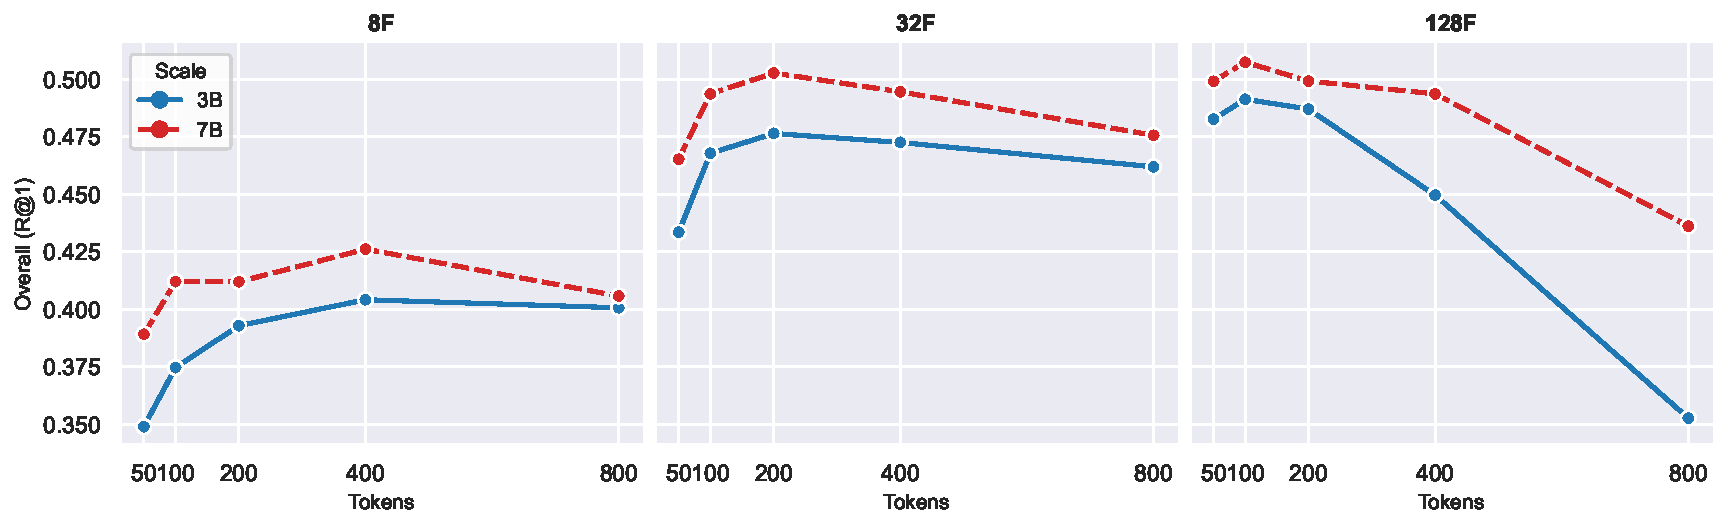
\includegraphics[width=\linewidth]{figures/mglvr/mglvr_testtime_spatial_scaling_1.pdf}
    \caption{Test-time spatial scaling sensitivity of GVE at temporal densities $F \in \{8, 32, 128\}$ frames per video. Each panel fixes $F$ and varies the number of spatial tokens $T$ per frame.}
    \label{mglvr:fig:spatial_scaling}
\end{figure}

\paragraph{Temporal Scaling.}
Varying $F$ from 4 to 512 frames reveals a divergence in scaling behavior across model families (Figure~\ref{mglvr:fig:temporal_scaling}). MLLM-based models exhibit continuous improvement up to $F = 128$, with the largest absolute gains on FN queries. CLIP-based models, by contrast, plateau around $F = 16$ and exhibit performance degradation on FN and MD queries at higher frame counts. This difference is consistent with the underlying architectural design: MLLM-based models process frames jointly through a transformer with positional encodings, whereas CLIP-based models aggregate frame-level features via mean pooling, which dilutes discriminative signals as $F$ increases.

\paragraph{Spatiotemporal Trade-off.}
When $N_{\text{total}}$ is held constant, the optimal allocation between $F$ and $T$ depends on query granularity (Figure~\ref{mglvr:fig:tradeoff}). CR queries favor high-resolution, low-frame-count configurations, while FN queries favor more frames at lower spatial resolution. Reducing spatial tokens primarily discards fine-grained texture while preserving semantic content, whereas reducing the number of frames risks eliminating visual evidence of brief events entirely.

\begin{sidewaysfigure}[t]
    \centering
    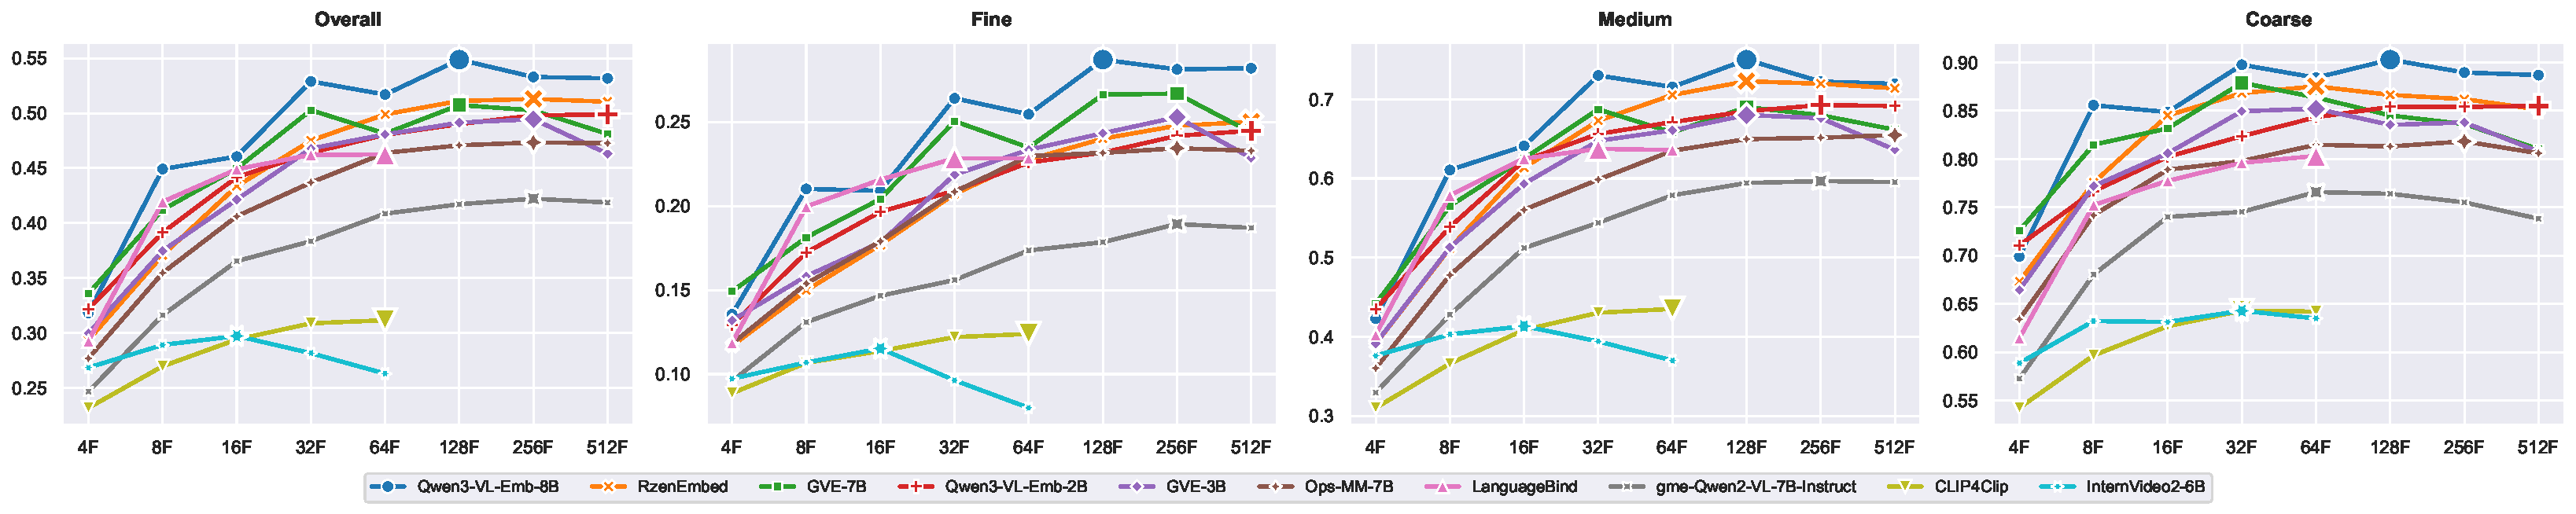
\includegraphics[width=\linewidth]{figures/mglvr/mglvr_testtime_temporal_scaling.pdf}
    \caption{Test-time temporal scaling across model families. MLLM-based models exhibit continuous improvement with increasing frame count, whereas CLIP-based models plateau and degrade at high frame counts.}
    \label{mglvr:fig:temporal_scaling}

    \vspace{1em}
    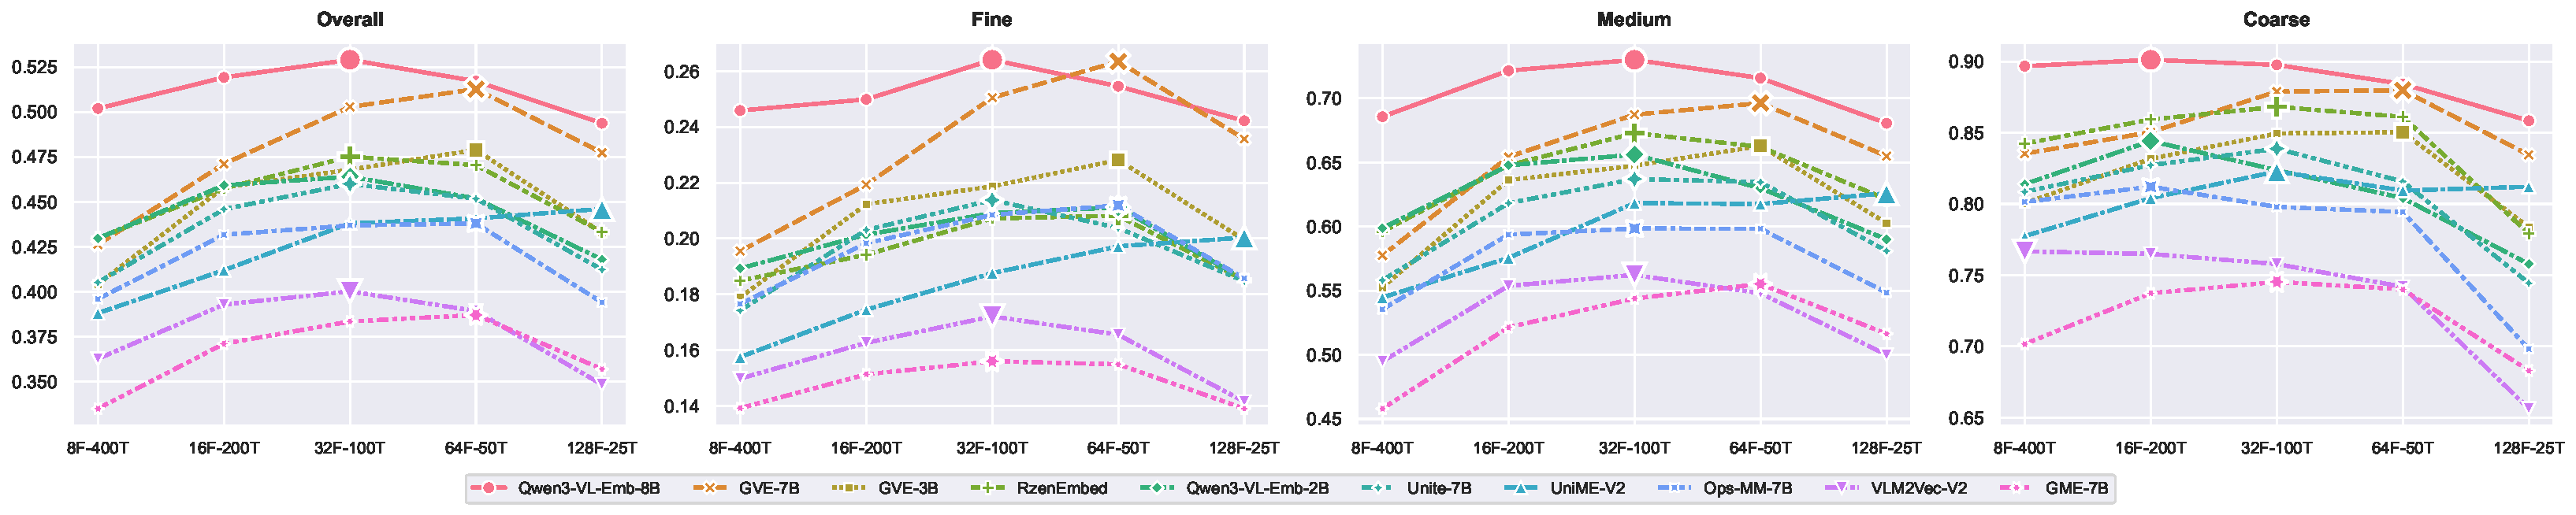
\includegraphics[width=\linewidth]{figures/mglvr/st_tradeoff.pdf}
    \caption{Retrieval performance under a fixed total token budget. The optimal allocation between spatial and temporal tokens shifts systematically with query granularity.}
    \label{mglvr:fig:tradeoff}
\end{sidewaysfigure}

\subsection{Training-Time Scaling}
\label{mglvr:sec:trainingtime}

Following the protocol of an existing work~\cite{guo2025gve}, we post-train Qwen2.5-VL-Instruct-3B~\cite{bai2025qwen25vl} with InfoNCE loss~\cite{oord2018representation} on 500K instances to examine how the training density $(F_{\text{train}}, T_{\text{train}})$ shapes the learned embedding space. We organize the results as two complementary comparisons. Table~\ref{mglvr:tab:train_spatial_scaling} varies the spatial training density and evaluates it at 4 and 8 test frames. Table~\ref{mglvr:tab:train_temporal_scaling} varies the temporal training density and evaluates it at 50 and 100 spatial tokens per test frame. Together, the two tables separate resolution robustness from frame-count anchoring.

\paragraph{Spatial Scaling: Resolution Robustness.}
Increasing $T_{\text{train}}$ yields consistent performance gains across most granularity levels and inference resolutions. Table~\ref{mglvr:tab:train_spatial_scaling}(a) reports evaluation at 4 test frames, and panel (b) verifies the same pattern at 8 test frames. Models trained at $T_{\text{train}} = 400$ achieve the best Overall R@1 in all four test-time spatial groups. Notably, even when evaluated at $T_{\text{test}} = 50$, the model trained at $T_{\text{train}} = 400$ substantially outperforms the model trained directly at $T_{\text{train}} = 50$ ($+0.0155$ Overall R@1). We term this property \textit{resolution robustness}: representations learned at high spatial density generalize effectively to low-density inference. However, this trend is not strictly monotonic at all granularity levels: at $T_{\text{test}} = 400$, increasing $T_{\text{train}}$ from 200 to 400 yields only marginal overall gains ($+0.0014$ Overall R@1) while slightly degrading Fine R@1 ($-0.0021$) and Coarse R@1 ($-0.0027$), suggesting diminishing returns at extreme spatial density.

\begin{table}[t]
    \centering
    \caption{Training-time spatial scaling with $F_{\text{train}}=4$, evaluated at (a) 4 and (b) 8 test frames. Models trained at $T_{\text{train}} \in \{50, 100, 200, 400\}$ are evaluated across all spatial test configurations. Bold indicates the best result within each group.}
    \label{mglvr:tab:train_spatial_scaling}
    \footnotesize
    \renewcommand{\arraystretch}{0.94}
    (a) Evaluation at 4 test frames.\par\smallskip
    \begin{tabular}{@{}c@{\hspace{3pt}}c@{\hspace{6pt}}c@{\hspace{3pt}}c@{\hspace{6pt}}*{7}{c@{\hspace{3pt}}}c@{}}
\toprule
\multicolumn{2}{c|}{Training} & \multicolumn{2}{c|}{Testing} & \multicolumn{2}{c|}{Overall} & \multicolumn{2}{c|}{FN} & \multicolumn{2}{c|}{MD} & \multicolumn{2}{c}{CR} \\
Temporal & Spatial & Temporal & Spatial & R@1   & MRR   & R@1   & MRR   & R@1   & MRR   & R@1   & MRR \\
\midrule
% --- Group 1: Test Spatial = 50T ---
\multirow{4}{*}{4F} & 50T & \multirow{4}{*}{4F} & \multirow{4}{*}{50T}  & 0.1941 & 0.2679 & 0.0731 & 0.1226 & 0.2591 & 0.3509 & 0.4613 & 0.5710 \\
& 100T & & & 0.2019 & 0.2770 & 0.0797 & 0.1298 & 0.2677 & 0.3617 & 0.4711 & 0.5811 \\
& 200T & & & 0.2060 & 0.2820 & 0.0837 & 0.1346 & 0.2714 & 0.3671 & 0.4773 & 0.5865 \\
& 400T & & & \textbf{0.2096} & \textbf{0.2851} & \textbf{0.0865} & \textbf{0.1378} & \textbf{0.2740} & \textbf{0.3687} & \textbf{0.4880} & \textbf{0.5939} \\
\midrule
% --- Group 2: Test Spatial = 100T ---
\multirow{4}{*}{4F} & 50T & \multirow{4}{*}{4F} & \multirow{4}{*}{100T} & 0.2243 & 0.3011 & 0.0865 & 0.1390 & 0.2996 & 0.3968 & 0.5236 & 0.6277 \\
& 100T & & & 0.2212 & 0.2979 & 0.0837 & 0.1375 & 0.2945 & 0.3901 & 0.5272 & 0.6299 \\
& 200T & & & 0.2384 & 0.3180 & 0.0922 & 0.1494 & 0.3182 & 0.4173 & 0.5565 & 0.6583 \\
& 400T & & & \textbf{0.2474} & \textbf{0.3262} & \textbf{0.0975} & \textbf{0.1558} & \textbf{0.3300} & \textbf{0.4267} & \textbf{0.5708} & \textbf{0.6696} \\
\midrule
% --- Group 3: Test Spatial = 200T ---
\multirow{4}{*}{4F} & 50T & \multirow{4}{*}{4F} & \multirow{4}{*}{200T} & 0.2406 & 0.3168 & 0.0890 & 0.1420 & 0.3199 & 0.4178 & 0.5833 & 0.6764 \\
& 100T & & & 0.2425 & 0.3202 & 0.0922 & 0.1473 & 0.3197 & 0.4187 & 0.5877 & 0.6820 \\
& 200T & & & 0.2454 & 0.3230 & 0.0948 & 0.1500 & 0.3238 & 0.4220 & 0.5877 & 0.6834 \\
& 400T & & & \textbf{0.2581} & \textbf{0.3385} & \textbf{0.1031} & \textbf{0.1628} & \textbf{0.3440} & \textbf{0.4425} & \textbf{0.5913} & \textbf{0.6910} \\
\midrule
% --- Group 4: Test Spatial = 400T ---
\multirow{4}{*}{4F} & 50T & \multirow{4}{*}{4F} & \multirow{4}{*}{400T} & 0.2503 & 0.3263 & 0.0926 & 0.1471 & 0.3353 & 0.4318 & \textbf{0.5975} & 0.6883 \\
& 100T & & & 0.2507 & 0.3285 & 0.0914 & 0.1501 & 0.3378 & 0.4332 & \textbf{0.5975} & 0.6898 \\
& 200T & & & 0.2561 & 0.3342 & \textbf{0.0984} & \textbf{0.1566} & 0.3431 & 0.4392 & 0.5966 & \textbf{0.6909} \\
& 400T & & & \textbf{0.2575} & \textbf{0.3359} & 0.0963 & 0.1563 & \textbf{0.3496} & \textbf{0.4442} & 0.5939 & 0.6889 \\
\bottomrule
\end{tabular}
\par\medskip
(b) Evaluation at 8 test frames.\par\smallskip
\begin{tabular}{@{}c@{\hspace{3pt}}c@{\hspace{6pt}}c@{\hspace{3pt}}c@{\hspace{6pt}}*{7}{c@{\hspace{3pt}}}c@{}}
\toprule
\multicolumn{2}{c|}{Training} & \multicolumn{2}{c|}{Testing} & \multicolumn{2}{c|}{Overall} & \multicolumn{2}{c|}{FN} & \multicolumn{2}{c|}{MD} & \multicolumn{2}{c}{CR} \\
Temporal & Spatial & Temporal & Spatial & R@1 & MRR & R@1 & MRR & R@1 & MRR & R@1 & MRR \\
\midrule
\multirow{4}{*}{4F} & 50T  & \multirow{4}{*}{8F} & \multirow{4}{*}{50T}  & 0.2523 & 0.3349 & 0.0941 & 0.1561 & 0.3438 & 0.4461 & 0.5779 & 0.6746 \\
                    & 100T &                      &                       & 0.2567 & 0.3392 & 0.1018 & 0.1620 & 0.3486 & 0.4512 & 0.5672 & 0.6685 \\
                    & 200T &                      &                       & 0.2702 & 0.3529 & 0.1130 & 0.1734 & 0.3607 & 0.4647 & 0.5948 & 0.6928 \\
                    & 400T &                      &                       & \textbf{0.2778} & \textbf{0.3610} & \textbf{0.1137} & \textbf{0.1780} & \textbf{0.3759} & \textbf{0.4773} & \textbf{0.6037} & \textbf{0.6991} \\
\midrule
\multirow{4}{*}{4F} & 50T  & \multirow{4}{*}{8F} & \multirow{4}{*}{100T} & 0.2773 & 0.3598 & 0.1028 & 0.1673 & 0.3793 & 0.4817 & 0.6322 & 0.7169 \\
                    & 100T &                      &                       & 0.2815 & 0.3612 & 0.1065 & 0.1683 & 0.3877 & 0.4851 & 0.6233 & 0.7122 \\
                    & 200T &                      &                       & 0.2907 & 0.3709 & 0.1107 & 0.1752 & 0.3993 & 0.4962 & 0.6447 & 0.7292 \\
                    & 400T &                      &                       & \textbf{0.3041} & \textbf{0.3871} & \textbf{0.1220} & \textbf{0.1897} & \textbf{0.4179} & \textbf{0.5169} & \textbf{0.6474} & \textbf{0.7357} \\
\midrule
\multirow{4}{*}{4F} & 50T  & \multirow{4}{*}{8F} & \multirow{4}{*}{200T} & 0.2889 & 0.3704 & 0.1037 & 0.1691 & 0.4015 & 0.5008 & 0.6500 & 0.7333 \\
                    & 100T &                      &                       & 0.2915 & 0.3721 & 0.1109 & 0.1740 & 0.4000 & 0.4991 & 0.6483 & 0.7341 \\
                    & 200T &                      &                       & 0.2970 & 0.3785 & 0.1105 & 0.1767 & 0.4085 & 0.5076 & 0.6670 & 0.7480 \\
                    & 400T &                      &                       & \textbf{0.3062} & \textbf{0.3883} & \textbf{0.1171} & \textbf{0.1851} & \textbf{0.4242} & \textbf{0.5224} & \textbf{0.6634} & \textbf{0.7453} \\
\midrule
\multirow{4}{*}{4F} & 50T  & \multirow{4}{*}{8F} & \multirow{4}{*}{400T} & 0.2936 & 0.3738 & 0.1041 & 0.1681 & 0.4090 & 0.5076 & 0.6616 & 0.7423 \\
                    & 100T &                      &                       & 0.2977 & 0.3778 & 0.1124 & 0.1754 & 0.4097 & 0.5086 & 0.6607 & 0.7435 \\
                    & 200T &                      &                       & 0.3001 & 0.3800 & 0.1171 & 0.1790 & 0.4090 & 0.5085 & 0.6652 & 0.7488 \\
                    & 400T &                      &                       & \textbf{0.3058} & \textbf{0.3861} & \textbf{0.1203} & \textbf{0.1843} & \textbf{0.4198} & \textbf{0.5175} & \textbf{0.6625} & \textbf{0.7469} \\
\bottomrule
\end{tabular}
\end{table}

\FloatBarrier
\paragraph{Temporal Scaling: Frame-Count Anchoring.}
Unlike spatial representations, temporal representations are tightly coupled to the frame count seen during training, a phenomenon we term \textit{frame-count anchoring}. Table~\ref{mglvr:tab:train_temporal_scaling} shows that the pattern persists when evaluated at 50 and 100 spatial tokens per frame in panels (a) and (b), respectively. A mismatch between $F_{\text{train}}$ and $F_{\text{test}}$ consistently degrades performance in both directions, but the degradation is asymmetric. When $F_{\text{train}} \gg F_{\text{test}}$, the performance drop is more severe: a model trained at $F_{\text{train}} = 32$ and evaluated at $F_{\text{test}} = 4$ drops $0.0104$ in Fine R@1 relative to the matched $F_{\text{train}} = 4$ baseline (Group~1 in Table~\ref{mglvr:tab:train_temporal_scaling}(a)). In the inverse direction, a model trained at $F_{\text{train}} = 4$ and evaluated at $F_{\text{test}} = 32$ drops $0.0083$ in Fine R@1 relative to the matched $F_{\text{train}} = 32$ baseline (Group~4 in Table~\ref{mglvr:tab:train_temporal_scaling}(a)). Although these gaps are measured against different absolute performance levels and should be interpreted accordingly, the consistent pattern across groups suggests that low-frame-count training better preserves fine-grained discriminability under temporal mismatch than high-frame-count training does.

\begin{table}[t]
    \centering
    \caption{Training-time temporal scaling with $T_{\text{train}}=50$, evaluated at (a) 50 and (b) 100 spatial tokens per test frame. Models trained at $F_{\text{train}} \in \{4, 8, 16, 32\}$ are evaluated across six temporal test configurations. Bold indicates the best result within each group.}
    \label{mglvr:tab:train_temporal_scaling}
    \footnotesize
    \renewcommand{\arraystretch}{0.78}
    (a) Evaluation at 50 spatial tokens per test frame.\par\smallskip
    \begin{tabular}{@{}c@{\hspace{3pt}}c@{\hspace{6pt}}c@{\hspace{3pt}}c@{\hspace{6pt}}*{7}{c@{\hspace{3pt}}}c@{}}
\toprule
\multicolumn{2}{c|}{Training} & \multicolumn{2}{c|}{Testing} & \multicolumn{2}{c|}{Overall} & \multicolumn{2}{c|}{FN} & \multicolumn{2}{c|}{MD} & \multicolumn{2}{c}{CR} \\
Temporal & Spatial & Temporal & Spatial & R@1   & MRR   & R@1   & MRR   & R@1   & MRR   & R@1   & MRR \\
\midrule
% --- Group 1: Test Temporal = 4F ---
4F  & \multirow{4}{*}{50T} & \multirow{4}{*}{4F} & \multirow{4}{*}{50T} & 0.2076 & 0.2837 & 0.0841 & 0.1352 & \textbf{0.2706} & \textbf{0.3666} & 0.4924 & 0.6002 \\
8F  & & & & 0.2080 & 0.2842 & 0.0858 & 0.1374 & 0.2694 & 0.3654 & \textbf{0.4933} & \textbf{0.6004} \\
16F & & & & \textbf{0.2082} & \textbf{0.2854} & \textbf{0.0882} & \textbf{0.1396} & 0.2677 & 0.3659 & 0.4915 & 0.5987 \\
32F & & & & 0.1930 & 0.2687 & 0.0737 & 0.1261 & 0.2528 & 0.3466 & 0.4720 & 0.5792 \\
\midrule
% --- Group 2: Test Temporal = 8F ---
4F  & \multirow{4}{*}{50T} & \multirow{4}{*}{8F} & \multirow{4}{*}{50T} & 0.2639 & 0.3515 & 0.1054 & 0.1694 & 0.3566 & 0.4669 & 0.5859 & 0.6892 \\
8F  & & & & \textbf{0.2741} & \textbf{0.3605} & \textbf{0.1143} & \textbf{0.1788} & \textbf{0.3667} & \textbf{0.4764} & \textbf{0.6020} & \textbf{0.6946} \\
16F & & & & 0.2486 & 0.3295 & 0.0992 & 0.1591 & 0.3281 & 0.4291 & 0.5815 & 0.6763 \\
32F & & & & 0.2390 & 0.3168 & 0.0982 & 0.1531 & 0.3117 & 0.4095 & 0.5610 & 0.6614 \\
\midrule
% --- Group 3: Test Temporal = 16F ---
4F  & \multirow{4}{*}{50T} & \multirow{4}{*}{16F} & \multirow{4}{*}{50T} & 0.3165 & 0.4086 & 0.1207 & 0.1951 & 0.4464 & 0.5590 & 0.6581 & 0.7484 \\
8F  & & & & 0.3071 & 0.3941 & 0.1147 & 0.1839 & 0.4288 & 0.5363 & 0.6643 & 0.7501 \\
16F & & & & \textbf{0.3254} & \textbf{0.4136} & \textbf{0.1235} & \textbf{0.1972} & \textbf{0.4587} & \textbf{0.5648} & \textbf{0.6803} & \textbf{0.7628} \\
32F & & & & 0.3090 & 0.3987 & 0.1196 & 0.1903 & 0.4254 & 0.5385 & 0.6732 & 0.7560 \\
\midrule
% --- Group 4: Test Temporal = 32F ---
4F  & \multirow{4}{*}{50T} & \multirow{4}{*}{32F} & \multirow{4}{*}{50T} & 0.3310 & 0.4196 & 0.1373 & 0.2088 & 0.4611 & 0.5678 & 0.6625 & 0.7559 \\
8F  & & & & 0.3556 & 0.4433 & 0.1432 & 0.2192 & 0.5017 & 0.6057 & 0.7070 & 0.7831 \\
16F & & & & 0.3574 & 0.4466 & \textbf{0.1466} & \textbf{0.2255} & 0.5034 & 0.6068 & 0.7026 & 0.7820 \\
32F & & & & \textbf{0.3596} & \textbf{0.4476} & 0.1456 & 0.2224 & \textbf{0.5075} & \textbf{0.6118} & \textbf{0.7115} & \textbf{0.7857} \\
\midrule
% --- Group 5: Test Temporal = 64F ---
4F  & \multirow{4}{*}{50T} & \multirow{4}{*}{64F} & \multirow{4}{*}{50T} & 0.3829 & 0.4717 & 0.1655 & 0.2440 & 0.5328 & 0.6392 & \textbf{0.7409} & \textbf{0.8110} \\
8F  & & & & 0.3772 & 0.4640 & 0.1596 & 0.2375 & 0.5280 & 0.6294 & 0.7329 & 0.8031 \\
16F & & & & 0.3877 & 0.4746 & \textbf{0.1698} & \textbf{0.2488} & 0.5420 & 0.6421 & 0.7320 & 0.8026 \\
32F & & & & \textbf{0.3892} & \textbf{0.4769} & 0.1668 & 0.2472 & \textbf{0.5468} & \textbf{0.6472} & 0.7400 & \textbf{0.8110} \\
\midrule
% --- Group 6: Test Temporal = 128F ---
4F  & \multirow{4}{*}{50T} & \multirow{4}{*}{128F} & \multirow{4}{*}{50T} & 0.4021 & 0.4900 & 0.1772 & 0.2604 & 0.5633 & 0.6626 & 0.7498 & 0.8174 \\
8F  & & & & 0.3941 & 0.4799 & 0.1698 & 0.2511 & 0.5538 & 0.6500 & 0.7453 & 0.8116 \\
16F & & & & 0.4058 & 0.4939 & 0.1806 & 0.2651 & \textbf{0.5681} & \textbf{0.6661} & 0.7507 & 0.8174 \\
32F & & & & \textbf{0.4078} & \textbf{0.4949} & \textbf{0.1859} & \textbf{0.2695} & 0.5666 & 0.6629 & \textbf{0.7516} & \textbf{0.8195} \\
\bottomrule
\end{tabular}
\par\medskip
(b) Evaluation at 100 spatial tokens per test frame.\par\smallskip
\begin{tabular}{@{}c@{\hspace{3pt}}c@{\hspace{6pt}}c@{\hspace{3pt}}c@{\hspace{6pt}}*{7}{c@{\hspace{3pt}}}c@{}}
\toprule
\multicolumn{2}{c|}{Training} & \multicolumn{2}{c|}{Testing} & \multicolumn{2}{c|}{Overall} & \multicolumn{2}{c|}{FN} & \multicolumn{2}{c|}{MD} & \multicolumn{2}{c}{CR} \\
Temporal & Spatial & Temporal & Spatial & R@1 & MRR & R@1 & MRR & R@1 & MRR & R@1 & MRR \\
\midrule
4F  & \multirow{4}{*}{50T} & \multirow{4}{*}{4F}   & \multirow{4}{*}{100T} & \textbf{0.2426} & \textbf{0.3213} & \textbf{0.0935} & \textbf{0.1498} & \textbf{0.3230} & \textbf{0.4222} & \textbf{0.5708} & \textbf{0.6681} \\
8F  &                      &                       &                       & 0.2395 & 0.3189 & 0.0912 & 0.1490 & 0.3213 & 0.4193 & 0.5592 & 0.6609 \\
16F &                      &                       &                       & 0.2251 & 0.3008 & 0.0861 & 0.1408 & 0.2945 & 0.3891 & 0.5512 & 0.6456 \\
32F &                      &                       &                       & 0.2286 & 0.3031 & 0.0916 & 0.1440 & 0.2970 & 0.3908 & 0.5503 & 0.6459 \\
\midrule
4F  & \multirow{4}{*}{50T} & \multirow{4}{*}{8F}   & \multirow{4}{*}{100T} & 0.3116 & 0.3984 & 0.1232 & 0.1943 & 0.4336 & 0.5367 & 0.6509 & 0.7438 \\
8F  &                      &                       &                       & \textbf{0.3188} & \textbf{0.4027} & \textbf{0.1288} & \textbf{0.1979} & \textbf{0.4384} & \textbf{0.5390} & \textbf{0.6741} & \textbf{0.7582} \\
16F &                      &                       &                       & 0.2982 & 0.3828 & 0.1169 & 0.1846 & 0.4116 & 0.5126 & 0.6394 & 0.7345 \\
32F &                      &                       &                       & 0.3045 & 0.3892 & 0.1258 & 0.1925 & 0.4112 & 0.5151 & 0.6598 & 0.7493 \\
\midrule
4F  & \multirow{4}{*}{50T} & \multirow{4}{*}{16F}  & \multirow{4}{*}{100T} & 0.3549 & 0.4422 & 0.1392 & 0.2160 & 0.4988 & 0.6026 & \textbf{0.7284} & \textbf{0.7986} \\
8F  &                      &                       &                       & 0.3553 & 0.4426 & 0.1400 & 0.2172 & 0.5010 & 0.6035 & 0.7204 & 0.7942 \\
16F &                      &                       &                       & \textbf{0.3582} & \textbf{0.4454} & \textbf{0.1405} & \textbf{0.2176} & \textbf{0.5097} & \textbf{0.6114} & 0.7124 & 0.7882 \\
32F &                      &                       &                       & 0.3266 & 0.4116 & 0.1194 & 0.1896 & 0.4611 & 0.5642 & 0.6990 & 0.7793 \\
\midrule
4F  & \multirow{4}{*}{50T} & \multirow{4}{*}{32F}  & \multirow{4}{*}{100T} & 0.3860 & 0.4736 & 0.1619 & 0.2404 & 0.5432 & 0.6462 & 0.7453 & 0.8138 \\
8F  &                      &                       &                       & 0.3805 & 0.4663 & 0.1594 & 0.2362 & 0.5340 & 0.6345 & 0.7409 & 0.8104 \\
16F &                      &                       &                       & \textbf{0.3905} & \textbf{0.4783} & \textbf{0.1664} & \textbf{0.2465} & 0.5483 & \textbf{0.6496} & \textbf{0.7480} & \textbf{0.8179} \\
32F &                      &                       &                       & 0.3877 & 0.4741 & 0.1636 & 0.2434 & \textbf{0.5495} & 0.6457 & 0.7302 & 0.8078 \\
\midrule
4F  & \multirow{4}{*}{50T} & \multirow{4}{*}{64F}  & \multirow{4}{*}{100T} & 0.4086 & 0.4923 & 0.1728 & 0.2538 & \textbf{0.5799} & \textbf{0.6726} & 0.7649 & 0.8266 \\
8F  &                      &                       &                       & 0.3960 & 0.4809 & 0.1696 & 0.2485 & 0.5560 & 0.6530 & 0.7551 & 0.8199 \\
16F &                      &                       &                       & 0.4108 & 0.4961 & 0.1832 & 0.2627 & 0.5739 & 0.6713 & 0.7631 & 0.8284 \\
32F &                      &                       &                       & \textbf{0.4148} & \textbf{0.4994} & \textbf{0.1885} & \textbf{0.2693} & 0.5739 & 0.6699 & \textbf{0.7765} & \textbf{0.8347} \\
\midrule
4F  & \multirow{4}{*}{50T} & \multirow{4}{*}{128F} & \multirow{4}{*}{100T} & 0.4130 & 0.4970 & 0.1859 & 0.2660 & 0.5794 & 0.6723 & 0.7507 & 0.8186 \\
8F  &                      &                       &                       & 0.4013 & 0.4853 & 0.1764 & 0.2556 & 0.5618 & 0.6569 & 0.7516 & 0.8143 \\
16F &                      &                       &                       & 0.4167 & 0.5015 & 0.1840 & 0.2679 & \textbf{0.5843} & 0.6769 & 0.7738 & 0.8330 \\
32F &                      &                       &                       & \textbf{0.4226} & \textbf{0.5073} & \textbf{0.1951} & \textbf{0.2782} & \textbf{0.5843} & \textbf{0.6782} & \textbf{0.7801} & \textbf{0.8368} \\
\bottomrule
\end{tabular}
\end{table}

\FloatBarrier
\subsection{Error Analysis and Case Studies}
\label{mglvr:sec:error_analysis}

The aggregate scaling results reveal how performance changes with sampling density, but they do not show how individual failures arise. Figure~\ref{mglvr:fig:error_cases} summarizes three representative retrieval cases that delimit both the benefits and the limitations of spatiotemporal scaling.

\paragraph{Degradation on Long Continuous Temporal Segments.}
As shown in Figure~\ref{mglvr:fig:error1}, performance degrades on long, continuous events. A fixed-length context window, such as 16 frames, divides a long video into short and independently processed clips, which can prevent the representation from capturing the full temporal scope of events spanning multiple clips.

\paragraph{Failure in Fine-Grained Temporal Retrieval.}
Figure~\ref{mglvr:fig:error2} shows a case in which the target event is a brief scene in the background. This resembles a needle-in-a-haystack setting, where increasing temporal coverage can improve the chance of observing the event but does not guarantee that the representation will preserve it strongly enough for retrieval.

\paragraph{Incomplete Satisfaction of Semantic Constraints.}
As shown in Figure~\ref{mglvr:fig:error3}, the model sometimes fails to satisfy all query conditions. The top-1 retrieved video satisfies the ``speaker'' requirement but does not match the ``blue background'' constraint. Similarly, the top-3 retrieved video satisfies most constraints but misses the requirement that the speaker wear a patterned shirt.

\begin{figure}[t]
  \centering
  \subfloat[]{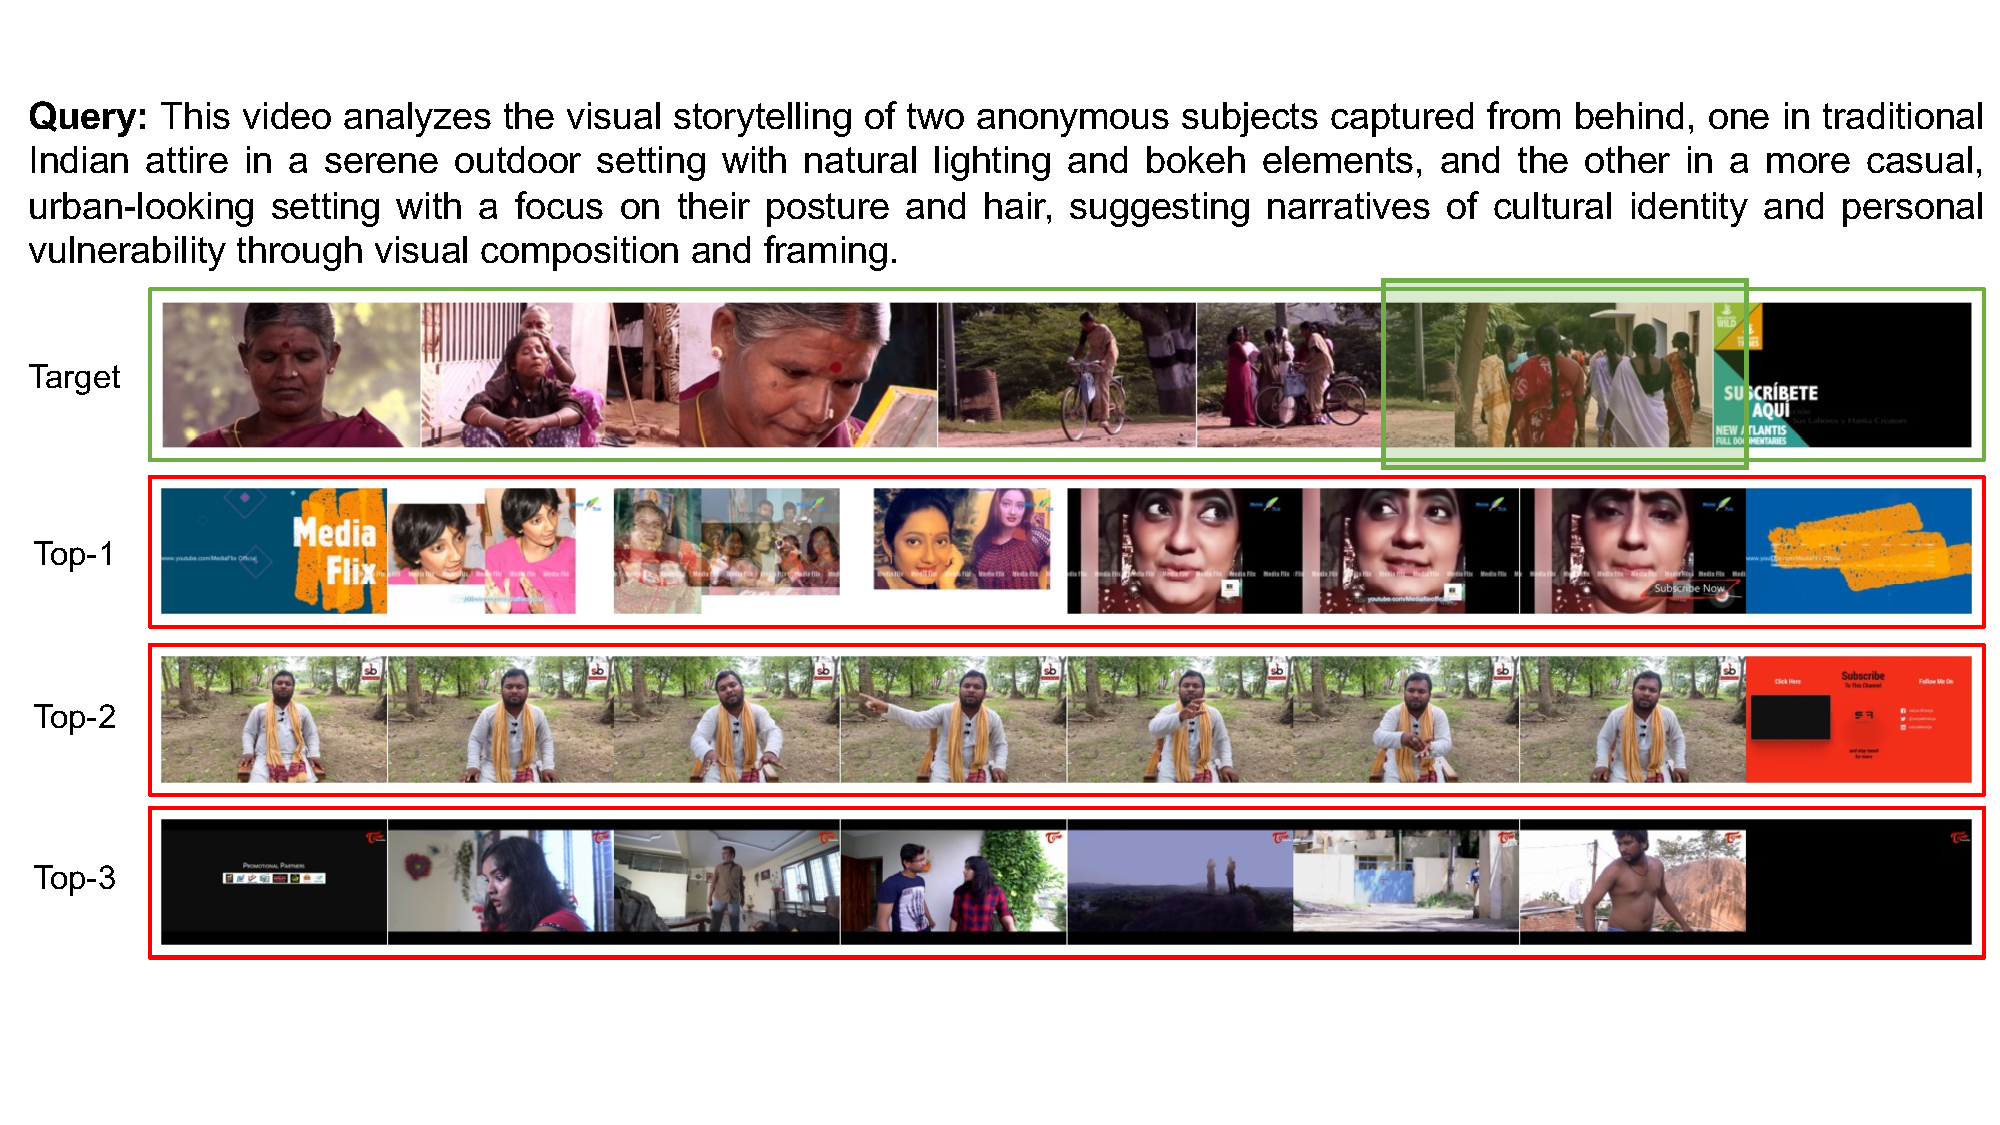
\includegraphics[width=\linewidth]{figures/mglvr/error-analysis/lvr-error-analysis-1.pdf}\label{mglvr:fig:error1}}\\[-0.5ex]
  \subfloat[]{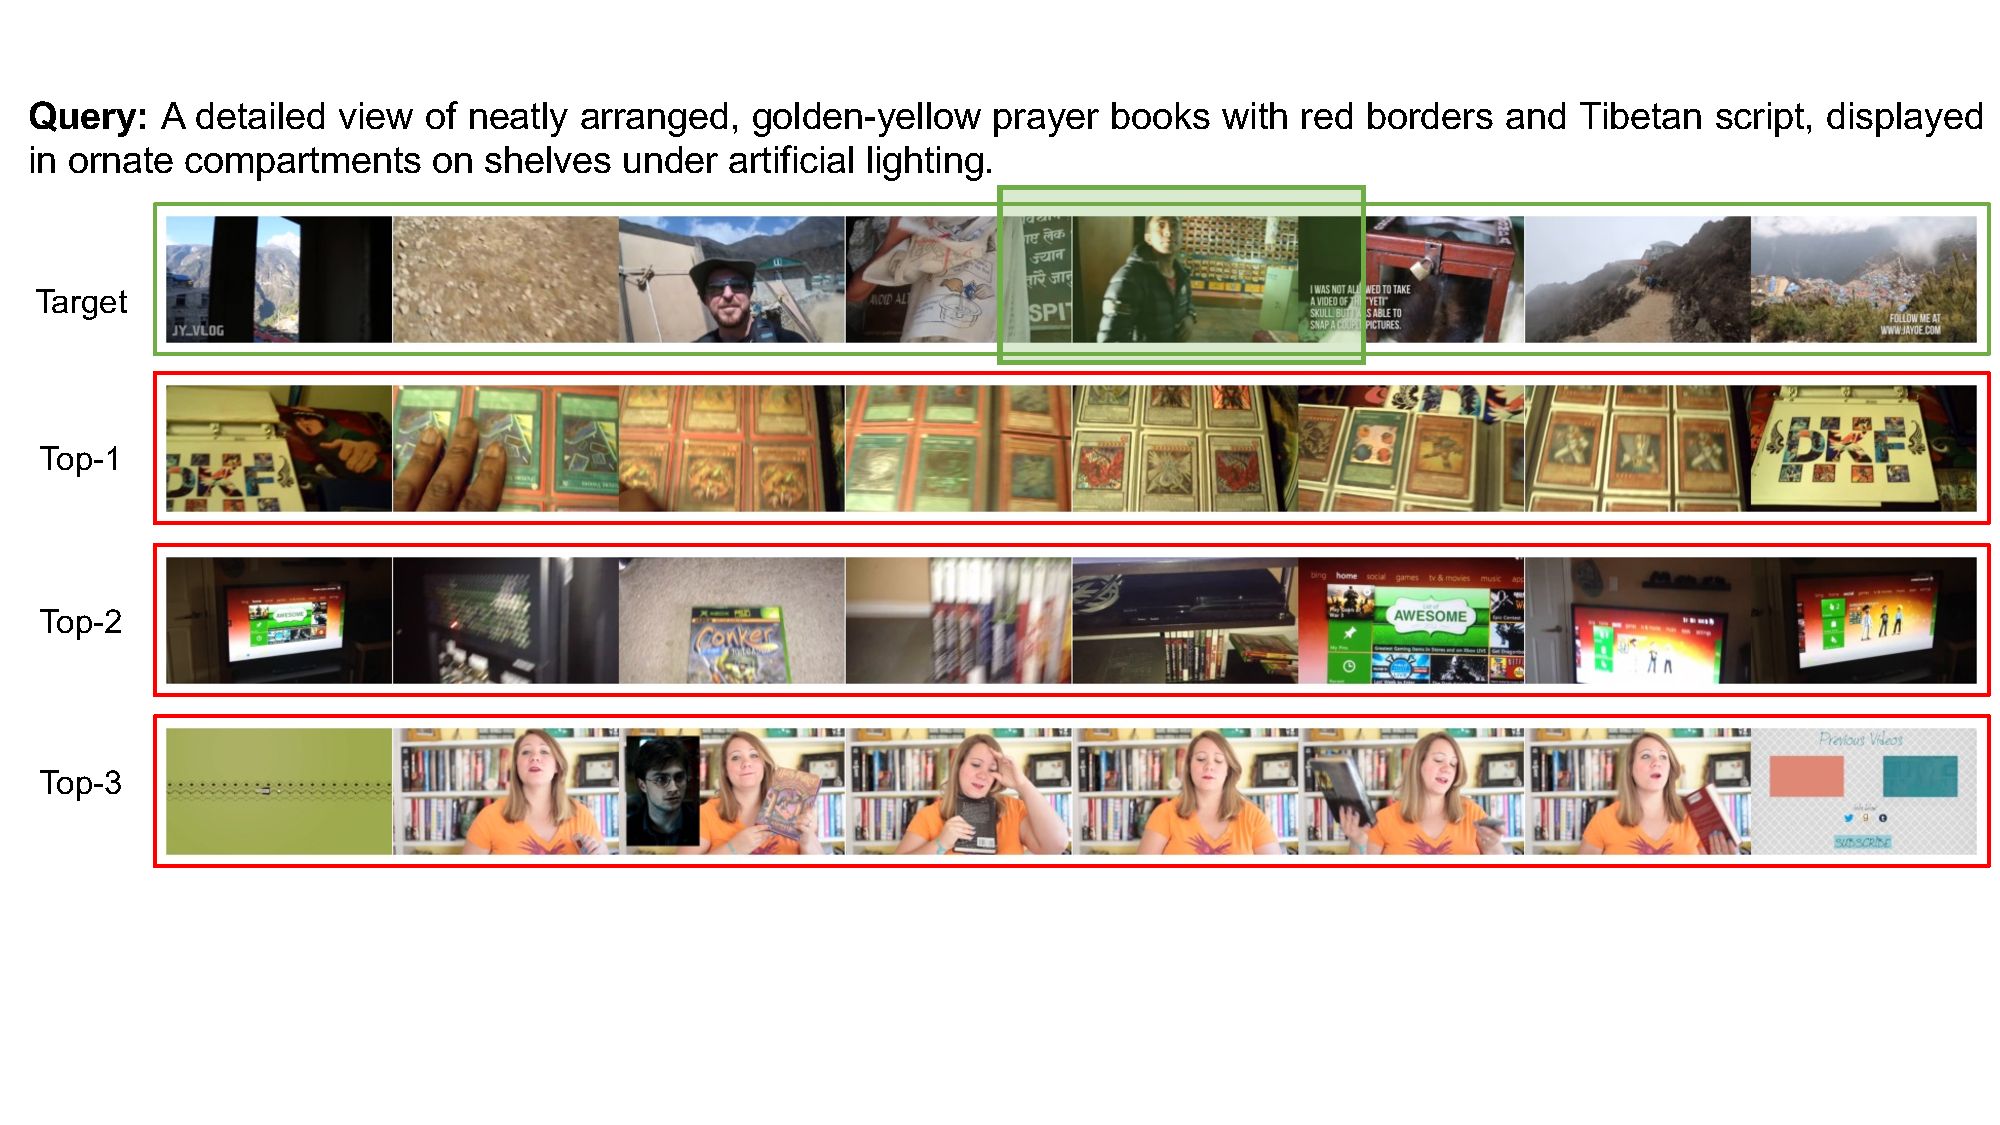
\includegraphics[width=\linewidth]{figures/mglvr/error-analysis/lvr-error-analysis-2.pdf}\label{mglvr:fig:error2}}\\[-0.5ex]
  \subfloat[]{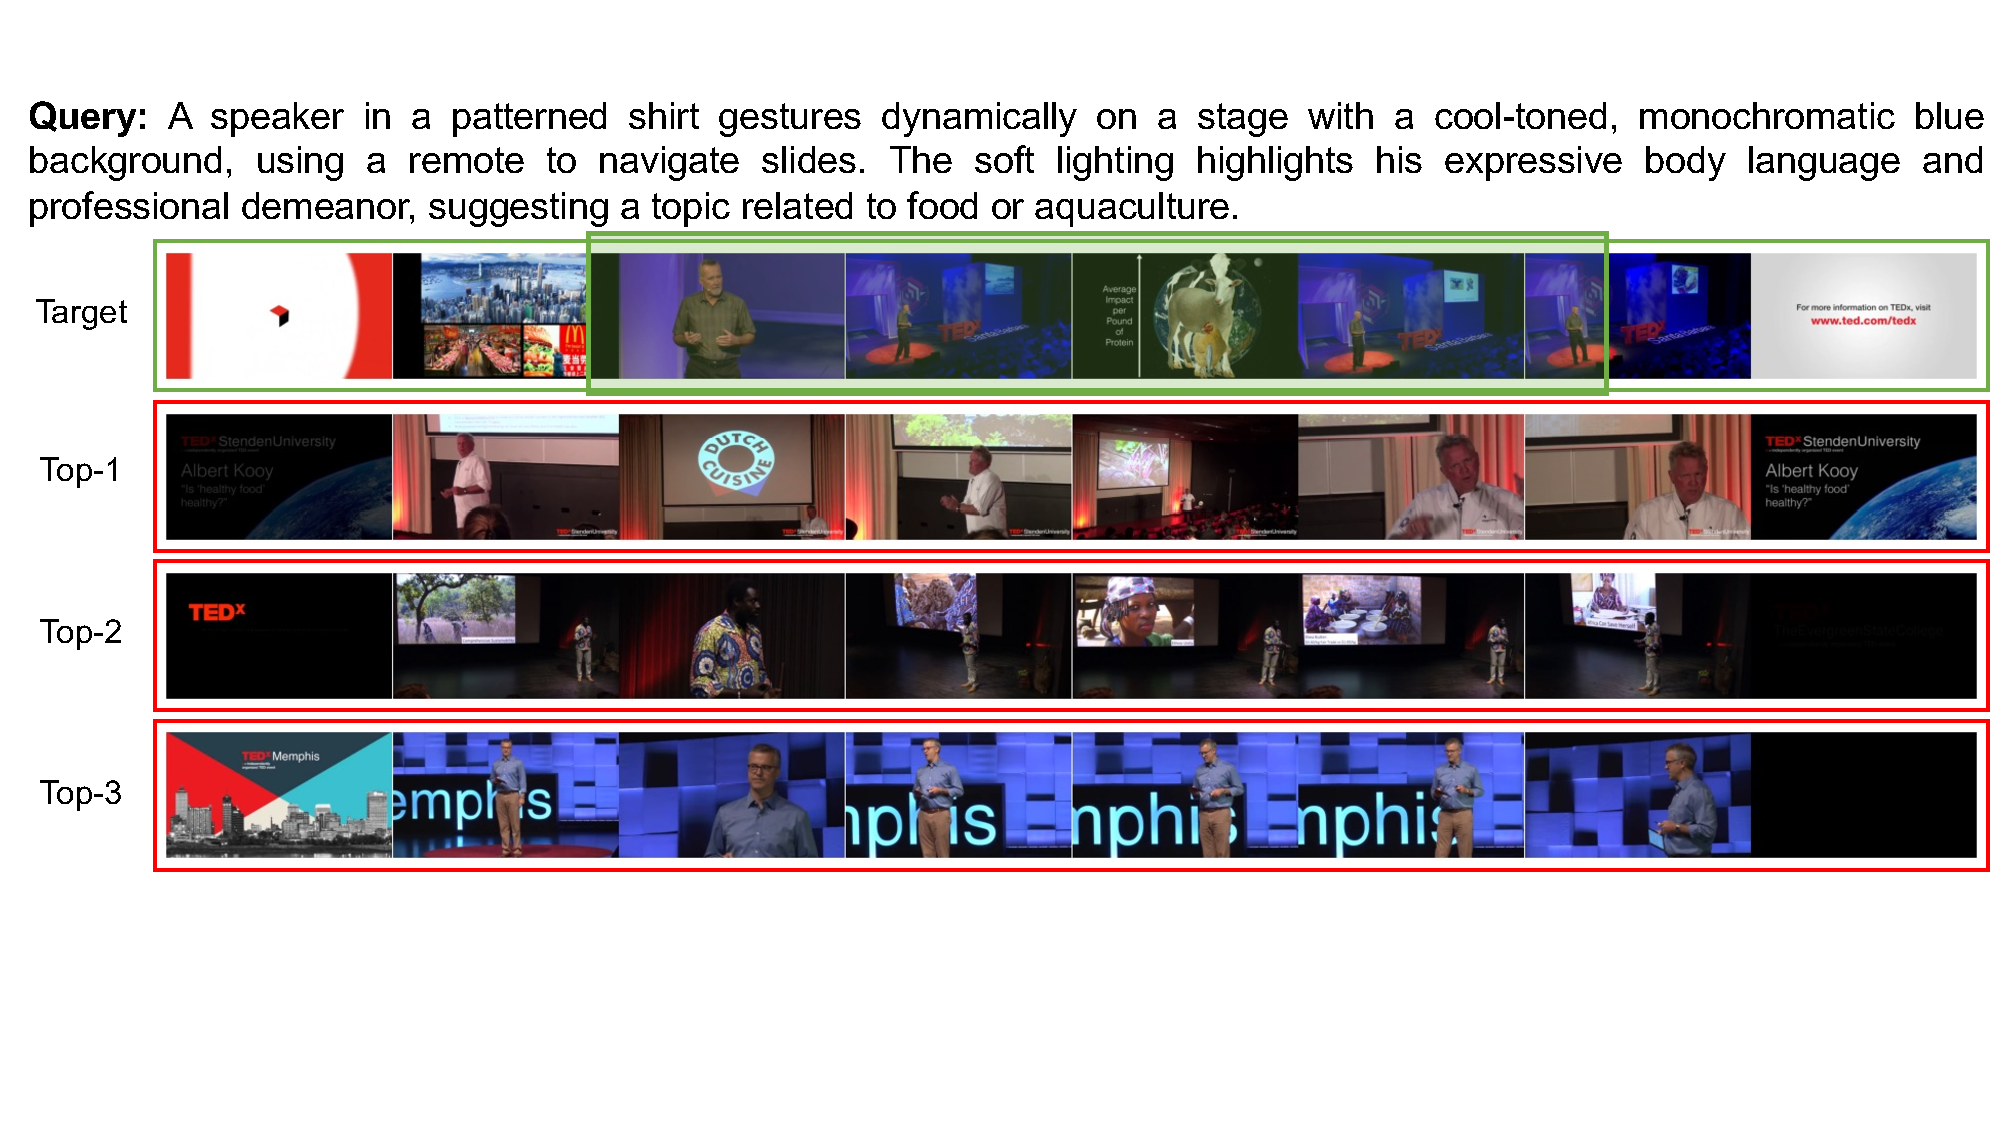
\includegraphics[width=\linewidth]{figures/mglvr/error-analysis/lvr-error-analysis-3.pdf}\label{mglvr:fig:error3}}
  \caption{Representative retrieval errors: (a) degradation on long continuous temporal segments, (b) failure in fine-grained temporal retrieval, and (c) incomplete satisfaction of semantic constraints.}
  \label{mglvr:fig:error_cases}
\end{figure}

\FloatBarrier
\section[VEterfall: Channeling Scaling Potential for Self-Enhancement of Video Embedding Models]{VEterfall: Channeling Scaling Potential for\\Self-Enhancement of Video Embedding Models}
\label{mglvr:sec:veterfall}

Our analysis reveals a key asymmetry: spatial embeddings tolerate token compression well, whereas temporal ones are governed by frame-count anchoring, i.e., models evaluated with high frame-density inputs degrade when the frame count is reduced at inference time. This suggests that the knowledge required for low-density inference is already latent within representations produced under high-density input sampling, but is not automatically transferred when the sampling configuration changes. We therefore propose \textbf{Video Embedding Waterfall (VEterfall)}, a progressive dense-to-sparse self-distillation framework that explicitly propagates this knowledge along the sampling-density axis, from high- to low-density configurations stage by stage, analogous to water descending through successive levels of a waterfall as shown in Figure~\ref{mglvr:fig:veterfall}.

\subsection{Method}

\paragraph{Single Dense-to-Sparse Distillation Step.}
The basic unit of VEterfall is a single distillation step~\cite{hinton2015distilling} from a denser to a sparser input sampling configuration, where density refers jointly to the number of frames sampled from the video and the number of spatial tokens retained per frame at inference time. A frozen teacher processes inputs at higher sampling density, while a student with the same architecture and initialization from the same pre-trained checkpoint $\mathcal{V}^{(0)}$ (here GVE-3B~\cite{guo2025gve}) is trained at a strictly lower density. The student is optimized to align its video embedding with that of the teacher via MSE loss, with an additional InfoNCE~\cite{oord2018representation} loss term ($\lambda{=}0.5$) to maintain video-text alignment by contrastive learning throughout density reduction.

\begin{figure}[t]
    \centering
    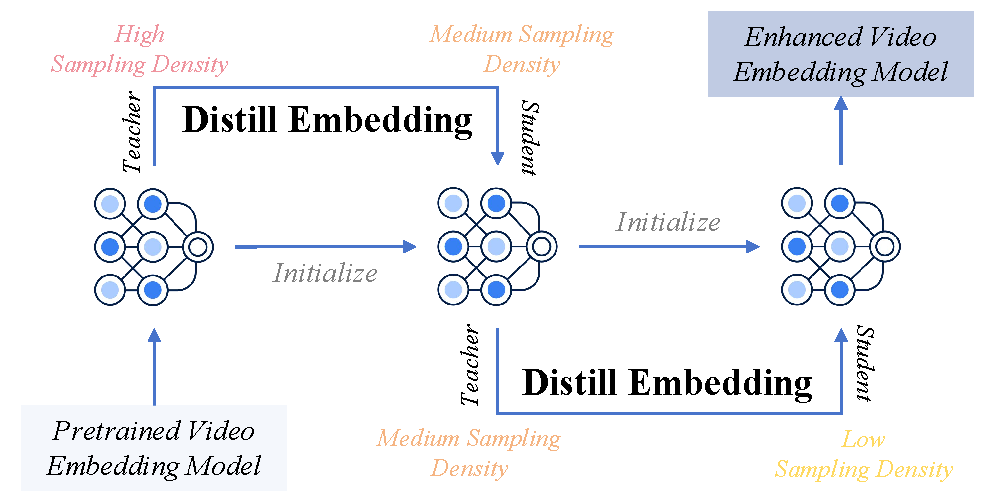
\includegraphics[width=0.75\linewidth]{figures/mglvr/d2s.pdf}
    \caption{VEterfall progressively distills video embeddings across progressively sparser input sampling configurations using the pretrained model itself as the teacher at each stage.}
    \label{mglvr:fig:veterfall}
\end{figure}

\paragraph{$K$-Round Cascade.}
To support large overall density reductions while keeping each individual step within a reliable transfer range, VEterfall chains $K$ distillation steps into a cascade, where each round takes the previous checkpoint as its frozen teacher:
\begin{equation*}
\mathcal{V}^{(k)} \xleftarrow{\;\text{distill}\;} \mathcal{V}^{(k-1)},
\qquad k = 1, \dots, K.
\end{equation*}
Here $\mathcal{V}^{(0)}$ serves as the pre-trained video embedding model, and $K$ controls the granularity of the reduction schedule.

\paragraph{Instantiation.}
We set $K{=}2$. Starting from $\mathcal{V}^{(0)}$ at $(16\text{F},\,400\text{T})$, the first round produces $\mathcal{V}^{(1)}$ at $(8\text{F},\,200\text{T})$, and the second produces $\mathcal{V}^{(2)}$ at $(4\text{F},\,100\text{T})$. Across two rounds, the input token budget is reduced by $16\times$ with no modification to the inference architecture. Each round uses 100K text-video pairs from InternVid~\cite{wang2023internvid}, a substantially smaller data requirement than comparable models.

\subsection{Experiments}

\begin{table}[t]
    \centering
    \caption{\textbf{Iterative Distillation.} R@1 performance across successive rounds ($K=1, 2$). VEterfall effectively recovers performance at lower densities, particularly for fine-grained queries.}
    \label{mglvr:tab:distillation}
    \begin{tabular}{@{}ll|*{4}{c}@{}}
        \toprule
        Setting & Model & Overall & Fine & Medium & Coarse \\
        \midrule
        \multirow{3}{*}{16F-400T} 
          & $\mathcal{V}^{(0)}$ & 0.447 & 0.202 & 0.622 & \textbf{0.829} \\
          & $\mathcal{V}^{(1)}$ & \underline{0.454} & \underline{0.212} & \underline{0.628} & \underline{0.826} \\
          & $\mathcal{V}^{(2)}$ & \textbf{0.456} & \textbf{0.215} & \textbf{0.630} & 0.819 \\
        \cmidrule(lr){1-6}
        \multirow{3}{*}{8F-200T} 
          & $\mathcal{V}^{(0)}$ & 0.369 & 0.148 & 0.508 & \textbf{0.782} \\
          & $\mathcal{V}^{(1)}$ & \underline{0.398} & \underline{0.182} & \underline{0.540} & \underline{0.780} \\
          & $\mathcal{V}^{(2)}$ & \textbf{0.402} & \textbf{0.188} & \textbf{0.543} & 0.777 \\
        \cmidrule(lr){1-6}
        \multirow{3}{*}{4F-100T} 
          & $\mathcal{V}^{(0)}$ & 0.300 & \underline{0.132} & 0.391 & \underline{0.664} \\
          & $\mathcal{V}^{(1)}$ & \underline{0.300} & 0.130 & \underline{0.394} & \underline{0.664} \\
          & $\mathcal{V}^{(2)}$ & \textbf{0.325} & \textbf{0.158} & \textbf{0.423} & \textbf{0.667} \\
        \bottomrule
    \end{tabular}
\end{table}

\paragraph{Main Results.}
As shown in Table \ref{mglvr:tab:distillation}, each distillation round yields consistent R@1 gains, with improvements concentrated on fine- and medium-grained queries. This is consistent with our earlier finding that these granularities are most sensitive to frame sparsity. Coarse-grained performance remains stable across rounds, confirming that holistic scene understanding is already well-preserved at low density. At 4F-100T, $\mathcal{V}^{(2)}$ improves overall R@1 from 0.300 to 0.325, with a ${\sim}$20\% relative gain on fine-grained queries. $\mathcal{V}^{(2)}$ also yields a marginal improvement at the original high-density setting, suggesting that the contrastive loss term provides mild regularization as a beneficial side effect.

\begin{table}[t]
    \centering
    \caption{\textbf{Frame-Efficiency.} Evaluated at fixed $T=200$. VEterfall ($\mathcal{V}^{(1)}$) significantly improves performance as frame count $F$ decreases.}
    \label{mglvr:tab:frame_eff}
    \begin{tabular}{@{}ll|*{4}{c}@{}}
        \toprule
        Setting & Model & Overall & Fine & Medium & Coarse \\
        \midrule
        \multirow{2}{*}{16F-200T}
          & $\mathcal{V}^{(0)}$ & \textbf{0.458} & \textbf{0.212} & \textbf{0.636} & \textbf{0.832} \\
          & $\mathcal{V}^{(1)}$ & 0.446 & 0.211 & 0.615 & 0.811 \\
        \cmidrule(lr){1-6}
        \multirow{2}{*}{8F-200T}
          & $\mathcal{V}^{(0)}$ & 0.369 & 0.148 & 0.508 & \textbf{0.782} \\
          & $\mathcal{V}^{(1)}$ & \textbf{0.398} & \textbf{0.182} & \textbf{0.540} & 0.780 \\
        \cmidrule(lr){1-6}
        \multirow{2}{*}{4F-200T}
          & $\mathcal{V}^{(0)}$ & 0.303 & 0.125 & 0.403 & 0.677 \\
          & $\mathcal{V}^{(1)}$ & \textbf{0.319} & \textbf{0.138} & \textbf{0.420} & \textbf{0.706} \\
        \bottomrule
    \end{tabular}
\end{table}

\begin{table}[t]
    \centering
    \caption{\textbf{Token-Efficiency.} Evaluated at fixed $F=8$. Benefits are consistent but less pronounced than frame-count adjustments.}
    \label{mglvr:tab:token_eff}
    \begin{tabular}{@{}ll|*{4}{c}@{}}
        \toprule
        Setting & Model & Overall & Fine & Medium & Coarse \\
        \midrule
        \multirow{2}{*}{8F-400T}
          & $\mathcal{V}^{(0)}$ & 0.404 & 0.179 & 0.553 & \textbf{0.801} \\
          & $\mathcal{V}^{(1)}$ & \textbf{0.412} & \textbf{0.191} & \textbf{0.558} & 0.800 \\
        \cmidrule(lr){1-6}
        \multirow{2}{*}{8F-200T}
          & $\mathcal{V}^{(0)}$ & 0.369 & 0.148 & 0.508 & \textbf{0.782} \\
          & $\mathcal{V}^{(1)}$ & \textbf{0.398} & \textbf{0.182} & \textbf{0.540} & 0.780 \\
        \cmidrule(lr){1-6}
        \multirow{2}{*}{8F-100T}
          & $\mathcal{V}^{(0)}$ & 0.375 & 0.158 & 0.513 & \textbf{0.772} \\
          & $\mathcal{V}^{(1)}$ & \textbf{0.380} & \textbf{0.171} & \textbf{0.516} & 0.758 \\
        \bottomrule
    \end{tabular}
\end{table}

\paragraph{Frame-Efficiency.}
We fix $T{=}200$ and vary the number of sampled frames $F$ to isolate the effect of temporal sparsity and evaluate the effectiveness of $\mathcal{V}^{(1)}$. As summarized in Table \ref{mglvr:tab:frame_eff}, $\mathcal{V}^{(1)}$ consistently outperforms $\mathcal{V}^{(0)}$ at 8 frames and below, with gains growing as the frame budget tightens. This confirms that VEterfall is most effective in the low-frame regime relevant for efficient deployment.

\paragraph{Token-Efficiency.}
As shown in Table \ref{mglvr:tab:token_eff}, where we fix $F{=}8$ and vary $T$, $\mathcal{V}^{(1)}$ improves consistently across all spatial token budgets. However, the margins are smaller and more uniform compared to frame-efficiency gains, confirming that spatial token compression is a secondary factor relative to frame sparsity.

\begin{table}[t]
    \centering
    \caption{\textbf{Ablation on $\lambda$}. Impact of contrastive loss term weight on 8F-200T performance. $\lambda=0.5$ provides the best alignment balance.}
    \label{mglvr:tab:lambda}
    \begin{tabular}{@{}l*{4}{c}@{}}
        \toprule
        $\lambda$ & Overall & Fine & Medium & Coarse \\
        \midrule
        0   & 0.396 & 0.178 & 0.537 & \textbf{0.782} \\
        0.5 & \textbf{0.398} & \textbf{0.182} & \textbf{0.540} & 0.780 \\
        \bottomrule
    \end{tabular}
\end{table}

\paragraph{Ablation on Contrastive Learning.}
Table \ref{mglvr:tab:lambda} illustrates the impact of the loss weight $\lambda$. Setting $\lambda{=}0$ already yields competitive performance, and adding the InfoNCE term provides marginal but consistent gains. These results confirm that the primary source of improvement is the embedding distillation objective rather than the contrastive learning term.

Together with the frame- and token-efficiency results, this ablation shows that observational scaling can be improved by transferring high-density embedding knowledge into sparse configurations.

\FloatBarrier
\section{Chapter Summary}

This chapter addressed the observational-scaling stage of the thesis by examining how spatial and temporal sampling determine which evidence a video embedding can preserve. It introduced MG-LVR, a long-video retrieval benchmark that controls query granularity and temporal continuity. Baseline results at 8, 32, and 128 frames revealed a persistent gap between coarse- and fine-grained retrieval. The subsequent test-time and training-time analyses showed that spatial and temporal density have different effects. Spatial representations are comparatively robust across resolutions, while temporal representations exhibit frame-count anchoring and are more sensitive to mismatches between training and inference. The error analysis connected these aggregate patterns to missed brief events, fragmented temporal evidence, and partially satisfied semantic constraints.

The chapter then translated these observations into VEterfall, a progressive dense-to-sparse self-distillation method. Its improvements under low-frame and low-token settings showed that knowledge available at high observational density can be transferred to more efficient configurations. Within the thesis, this study follows Chapter~\ref{ch:universal-video-retrieval} by moving from semantic coverage to evidence acquisition. It also establishes the input-efficiency conditions required before large-scale retrieval can be considered. Efficient embedding generation does not by itself make the resulting relevance signal searchable over massive candidate collections, which motivates the search-scaling study in Chapter~\ref{ch:scale-efficient-retrieval}.

\chapter{Search Scaling for Web-Scale Recommendations}
\label{ch:scale-efficient-retrieval}

\section{Introduction}

Chapters~\ref{ch:universal-video-retrieval} and~\ref{ch:spatiotemporal-scaling} address what a video embedding should represent and how visual evidence should be supplied to it. Accurate embedding generation is still insufficient when the learned relevance signal must be evaluated over billions of candidates under strict latency and throughput constraints~\cite{zhu2018learning,liu2021jizhi}. This chapter addresses this final bottleneck, search scaling, through the joint design of the learned metric, graph traversal, and GPU execution. The relevant background is reviewed centrally in \S\ref{sec:bc-search} and \S\ref{sec:lr-search}.

Retrieval-and-ranking frameworks~\cite{cheng2016wide,ma2020off} reduce a massive item catalog to a compact candidate set before ranking and are widely used in industrial systems~\cite{covington2016deep,borisyuk2016casmos,eksombatchai2018pixie}. The retrieval stage must preserve relevance while avoiding exhaustive scoring, making the interaction between metric quality and search efficiency central to deployment-scale retrieval.

This chapter focuses on the retrieval stage in Baidu's web-scale recommendation scenarios, e.g., news feed, Tieba, and video clips. Recent works~\cite{tan2020fast,chen2022approximate} establish the retrieval framework in a training-and-search manner.
Based on the complex relational dependencies modeling ability of Deep Neural Network~(DNN)~\cite{zhang2019deep}, they attempt to train a DNN-based metric for more accurate user-item relevance estimation compared with simple functions~\cite{dehghani2017neural,tay2018latent}.
Nevertheless, real-time retrieval is difficult due to complicated neural computations on massive candidates.
To solve the problem, researchers have been exploring the potential of Approximate Nearest Neighbor Search~(ANNS) algorithms to mitigate extensive computations, which search for relatively relevant items for each query user by selectively visiting instead of the entire item base.
Early works propose tree-based ANNS to organize data points in a tree-like structure by recursively splitting the dimensional space~\cite{friedman1977algorithm}.
However, they underperform in web-scale recommendations that aim to retrieve divergent and high-dimensional information because they are sensitive to complex feature spaces and item relationships~\cite{wang2021comprehensive}.
To improve retrieval effectiveness, the latest frameworks leverage graph-based ANNS algorithms that build similarity-based candidate graphs to efficiently expand the candidate set via graph traversal.
For example, HNSW~\cite{malkov2018efficient} hierarchically establishes a multi-layer indexing graph, grounding coarse-to-fine navigation towards the most satisfactory candidates.


However, we confront three challenges in developing an accurate and efficient retrieval framework for web-scale recommendations.
\textit{(1)~Unified modeling of multi-relational user-item relevance.} Baidu recommendation applications consist of dozens of distinct and related behaviors~(e.g., click, browse) that are typically modeled by a tailored metric for estimating relevance between users and items. However, the independent modeling of these user-item interactions fails to capture the semantic relations of diverse user behaviors, which are mutually beneficial between them~\cite{tan2020fast}. Besides, training multiple behavior-specific metrics incurs exponential efforts in system updates. Thus, the first challenge lies in cost-effective multi-relational metric joint training for more accurate relevance estimation.
\textit{(2)~Efficient search on large-scale graph item base.} Baidu devises Graph-based ANNS to traverse relevant candidate items from a graph item base. Practically, a trade-off problem arises that increasing the online retrieval throughput will restrict the search efforts, \ie, the graph traversal steps. However, existing methods make delivering satisfactory items in limited steps difficult, especially for billion-scale graphs in web-scale recommender systems.
On the one hand, neural relevance metrics often violate the triangle inequality, weakening the geometric consistency that supports efficient proximity-graph navigation~\cite{chen2022approximate}. This mismatch can force the exploration of redundant edges, decreasing the possibility of reaching distant yet relevant candidates.
On the other hand, graph-based ANNS usually search for relevant items greedily, which may be stuck in a narrow space after a short-length traversal among a large-scale graph.
The inability to balance search depth and breadth degrades the quality of real-time recommendations. Addressing this challenge requires developing a search-compatible relevance metric and a deep-and-broad traversal algorithm for efficient graph search.
\textit{(3)~Accelerating irregular neural computation in high concurrency.} At Baidu, users raise hundreds of millions of recommendation requests per second. These request executions are irregular because divergent user profiling drives distinct search paths, where the visited items should be estimated for their relevance by the neural metric. Baidu has developed a GPU-accelerated framework for web-scale recommendations to leverage the computational economy of GPUs~\cite{liu2022lion}. However, their performance degrades under highly concurrent, non-uniform workloads because of frequent kernel launches, a process with fixed latency overhead that dominates runtime when computations are small and irregular~\cite{el2016klap}. Millions of sequential processes of deep relevance computations on a GPU cluster introduce bottlenecks of recommendation throughput. Therefore, the third challenge is redesigning computation scheduling to accelerate large-scale irregular neural computations for higher throughput.

\begin{figure}[t]
    \centering
    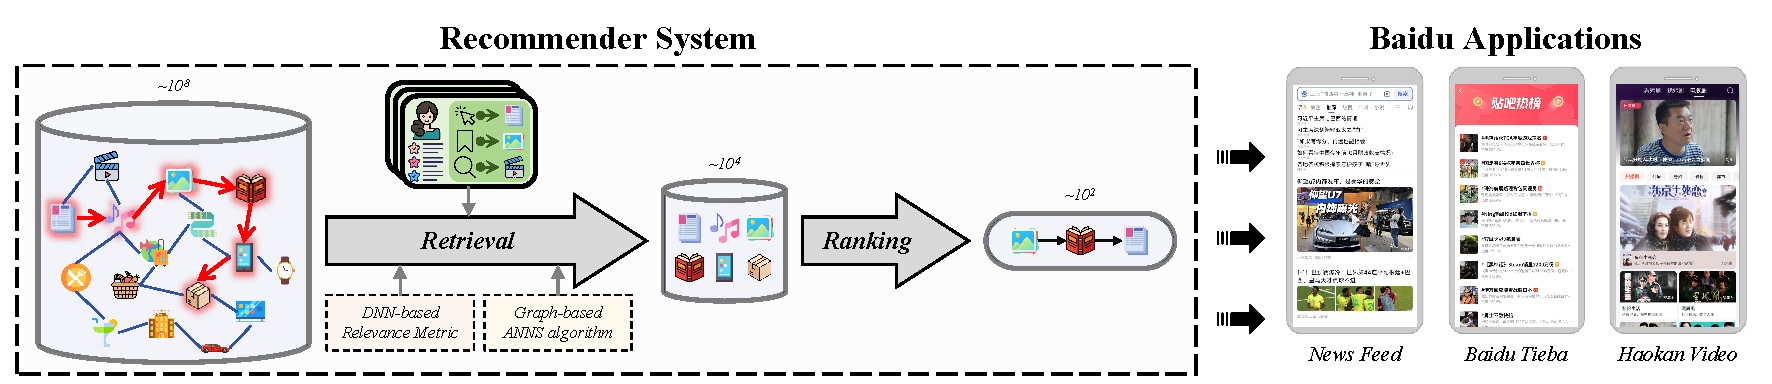
\includegraphics[width=\linewidth]{figures/gmpgr/Application.pdf}
    \caption{Applications of recommender systems at Baidu.}
    \label{gmpgr:fig:application}
\end{figure}

For the application scenarios shown in Figure~\ref{gmpgr:fig:application}, we propose a \textbf{GPU-accelerated Multi-relational Parallel Graph Retrieval~(GMP-GR)} framework for effective and efficient retrieval in web-scale recommendations.
Specifically, we first devise a \textit{Multi-relational User-Item Relevance Metric Learning~(MUIRML)} to generate a practical DNN-based metric via multi-objective optimization.
The metric extracts multi-relational knowledge in inter-dependent user behaviors to capture nuanced user preferences for accurate relevance measurement.
We also use a self-covariant loss to align the ranking regularity of our metric with Euclidean distance, encouraging shorter navigation paths on large graphs.
Second, we design a \textit{Hierarchically Parallel Approximate Nearest Neighbor Search~(HiPANNS)} algorithm to achieve timely and accurate retrieval for highly concurrent queries.
HiPANNS broadens the search space of the large graph item base by divergent parallel and co-optimized search processes, which can efficiently generate more relevant candidates in real-time retrieval.
Based on it, HiPANNS accelerates irregular neural computations from asynchronous requests by adaptive aggregation in a GPU-based cluster for higher retrieval throughput.
In Baidu recommendation applications, we further apply several system optimization strategies, including traffic dispersal, compilation optimization, model quantization, and timely stream update.
Extensive experiments demonstrate the superior retrieval effectiveness and efficiency of GMP-GR in offline retrieving evaluations and online recommendation services.
Our framework has been deployed in more than twenty web-scale recommender systems at Baidu, where it efficiently handles hundreds of millions of requests per second, improving user time-on-page by more than $3\%$ for hundreds of millions of users.

The contributions of this chapter are summarized as follows:
(1)~We propose a GPU-accelerated Multi-relational Parallel Graph Retrieval framework to achieve accurate and efficient retrieval for web-scale recommendations.
(2)~We devise a DNN-based metric to estimate user-item relevance via capturing inter-dependency among complex user-item relations, which can also improve the search efficiency on a large-scale graph for shorter navigation.
(3)~We design a GPU-accelerated parallel graph-based ANNS algorithm for highly concurrent retrieval by billion-scale breadth-depth balanced graph search and parallel irregular computations with adaptive aggregation.
(4)~We conduct extensive experiments to demonstrate retrieval effectiveness and efficiency improvements in offline and online recommendations at Baidu.


\section{Preliminaries}

Baidu has developed a recommendation framework as a comprehensive funnel mechanism to efficiently retrieve and rank items for users from a web-scale database for over twenty internet products~(e.g., news feed, short video clips, search engine, and online advertising)~\cite{liu2021jizhi}.
The recommendation framework has served hundreds of millions of online recommendation requests per second for hundreds of millions of users.
Next, we detail the retrieval framework for Baidu recommendations, including the retrieval problem and the retrieval pipeline.

\subsection{Online Retrieval at Baidu}
This setting instantiates the unified ranking problem in \S\ref{sec:bc-vr} at deployment scale. A user request serves as the query, the item base serves as the candidate corpus, and the learned relevance value determines the top-$K$ ordering. The notation below is specific to the industrial recommendation setting.

Given a user set $\mathcal{U}=\{u_1,u_2,\cdots,u_{N_u}\}$ and an item set $\mathcal{V}=\{v_1,v_2,\cdots,v_{N_v}\}$, consider a query from a user $u$ with raw feature $x_{u}$. The objective of the retrieval stage is to recommend the top-$K$ items that are most relevant to $u$ in order.
Specifically, we define the retrieval problem as a function $\mathcal{F}(\cdot;\cdot)$ that generates a set $V_{u}$ based on the user features. $V_u$ contains the $K$ most similar items $V_{u} = \{v_{u,1},v_{u,2},\cdots,v_{u,K}\}$ as
\begin{equation}
    V_{u} = \mathcal{F}(x_{u};\{v_1,v_2,\cdots,v_{N_v}\}).
\end{equation}

\subsection{Retrieval Pipeline at Baidu}

Baidu has constructed a graph retrieval framework in their recommendation system, including two stages: offline training and online search~\cite{tan2020fast,chen2022approximate}.

\subsubsection{Step 1. Offline Training}
The first stage aims to learn user and item embeddings associated with a relevance metric for estimating the relevance between users and items.
Embeddings and the metric are learnable modules stored by the system, which are immutable in the search stage.
We can also periodically re-train the modules once the properties change significantly.
Overall, the pipeline of the training step is presented below.

\textit{(1)~Users and item feature construction.}
We first prepare the raw features of the users and items that are denoted as $\{x_{u_1},x_{u_2},\cdots,x_{N_u}\}$ and $\{x_{v_1},x_{v_2},\cdots,x_{N_v}\}$, where $N_u$ and $N_v$ are the numbers of users and items, respectively. Meanwhile, the interaction records of users $u$ and items $v$ are denoted as $\{D^z_{u,v}\}$. For an interaction type $z$, $D^z_{u_i,v_j}$ is the interactive value between a user $u_i$ and an item $v_j$, which reflects how close they are in terms of the interaction $z$.

\textit{(2)~User and item embedding projection.}
Then, we pre-define a user and an item projector, $\mathcal{H}_u(\cdot)$ and $\mathcal{H}_v(\cdot)$, to transform raw features into learnable embeddings as user and item representations, which are defined as $h_{u_i} = \mathcal{H}_u(x_{u_i})$ and $h_{v_j} = \mathcal{H}_v(x_{v_j})$.

\textit{(3)~User-item relevance metric definition.}
After that, we devise a DNN-based learnable metric~\cite{dehghani2017neural,tay2018latent} to estimate the relevance between a user and an item by a high-dimensional calculation of their embeddings.
Hence, we aim to obtain a metric $\Delta(\cdot,\cdot)$ to quantify the relevance value given a user embedding and an item embedding as
\begin{equation*}
\delta_{u,v} = \Delta(h_u,h_v).
\end{equation*}

\textit{(4)~Optimization of embeddings and the metric.}
Next, we optimize the user embeddings, item embeddings, and the relevance metric based on the user features, item features, and user-item interactions. We describe the optimization as a function $\mathcal{F}_t(\cdot,\cdot,\cdot)$ that
\begin{equation}
    \{h_u\}, \{h_v\}, \Delta(\cdot,\cdot) = \mathcal{F}_t(\{x_u\}, \{x_v\}, \{D^z_{u,v}\}).
\end{equation}
The learned embeddings and the relevance metric are used in the online search stage to measure user-item relevance. 

\begin{figure}[t]
    \centering
    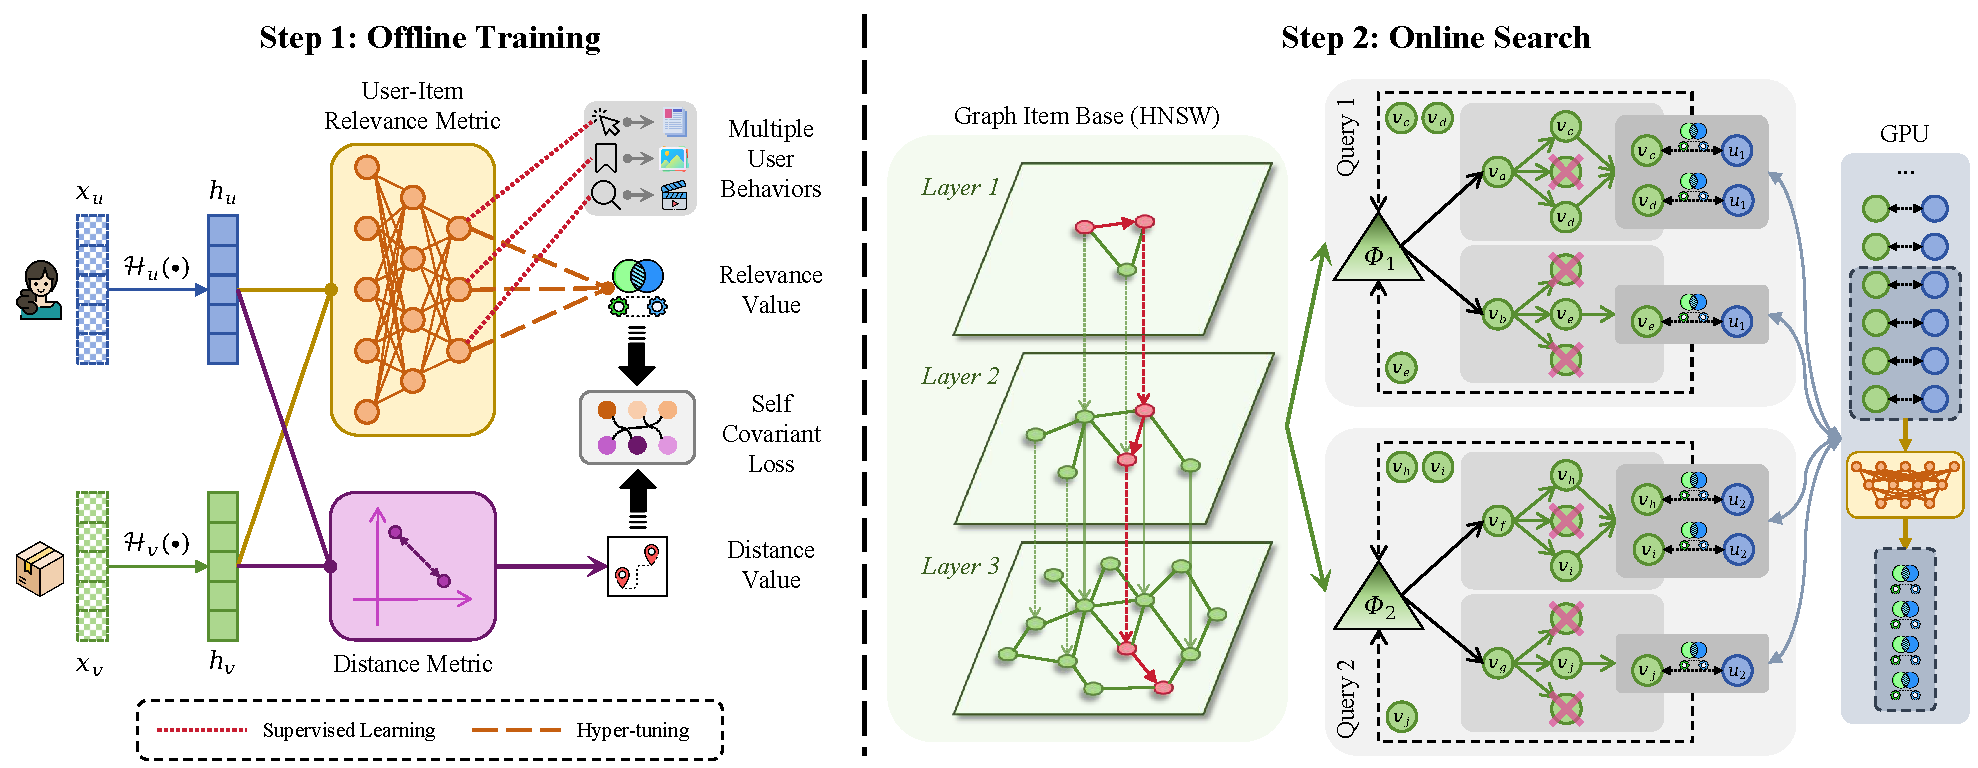
\includegraphics[width=\linewidth]{figures/gmpgr/GMP-GR.pdf}
    \caption{An overview of the GPU-accelerated Multi-relational Parallel Graph Retrieval framework.}
    \label{gmpgr:fig:gmp-gr}
\end{figure}


\subsubsection{Step 2. Online Search}
In the second stage, we construct a graph-based item database that supports an efficient search for the target items.
Traditional tree-based ANNS fails to handle web-scale data with high dimensions and uneven distributions, and requires extensive tree construction costs.
Instead, we follow graph-based ANNS to construct a graph item base that can efficiently navigate possibly relevant items and retrieve satisfactory items for given users based on graph search.
Specifically, we adopt HNSW~\cite{malkov2018efficient} as the graph structure.
HNSW utilizes a multi-layered graph structure, denoted as a $L$-layer graph $G$, where each upper layer contains fewer nodes to facilitate efficient search paths. Based on its hierarchy, we can effectively narrow the search space for nearest neighbors in the base layer, initiating the search process from the upper layers.

In the online search, we infer $K$ relevant items with a querying user as follows. We perform the search iteratively across each layer of the HNSW structure, with the selected items from one layer serving as seed nodes for traversal in the subsequent layer. For each layer, we first access the corresponding user embedding. Second, we generate seed nodes, from which we start to traverse the graph. Third, we expand the candidate node set by visiting neighbors of existing nodes and continuously update the most similar ones for the queried user. The $K$ most similar items are ultimately extracted from the final layer.
The overall search process for the relevant item set $\hat{V}_u$ for user $u$ can be defined as
\begin{equation}
    \hat{V}_u = \mathop{\arg\max}\limits_{\substack{V_u \subseteq \mathcal{V} \\ |V_u|=K}} \sum\limits_{v \in V_u} \delta_{u,v}.
\end{equation}


\section{GPU-accelerated Multi-relational Parallel Graph Retrieval Framework}

This section introduces the GPU-accelerated Multi-relational Parallel Graph Retrieval~(GMP-GR) framework deployed at Baidu for web-scale recommendation.
As shown in Figure~\ref{gmpgr:fig:gmp-gr}, GMP-GR equips two main modules to achieve effective and efficient performance.
In the training step, multi-relational user-item relevance metric learning generates a DNN-based metric that captures inter-dependent relationships between users and items while encouraging Euclidean ranking regularity for path-efficient graph search.
In the search step, a hierarchically parallel graph-based ANNS algorithm effectively delivers reliable search candidates in high concurrency, which explores a breadth-depth balanced search space and synchronizes large-scale irregular neural computations on GPUs.


\subsection{Multi-relational User-item Relevance Metric Learning}\label{gmpgr:sec:metric}

The training step aims to optimize the user and item embeddings with the DNN-based metric to model the relevance between users and items.
However, existing DNN-based metrics may model nuanced user preferences incompletely because they incorporate only part of the multi-dimensional behaviors on items, or may lack the geometric regularity that supports efficient graph-based ANNS navigation.
Therefore, we propose a \textit{Multi-relational User-Item Relevance Metric Learning~(MUIRML)} algorithm to train a relevance metric that not only ensures elaborate multi-relational modeling, but also enhances navigating efficiency in the search step, ultimately improving the retrieval effectiveness.

\textit{(1)~DNN-based Relevance computation.}
We first utilize a Multi-Layer Perceptron~(MLP) to model multiple interactive behaviors.
Initially, the input consists of the user embedding $h_u$, the item embedding $h_v$, and the serendipity vector $\tilde{h} \sim \mathcal{N}(0,1)$ for diverse exploration as
\begin{equation}
    h_{u,v}^{(0)} = \operatorname{concat}(h_u+\tilde{h},h_v),
\end{equation}
the MLP inputs $h_{u,v}^{(0)}$ and aims to output the interaction vector $Z_{u,v}$ that stacks multiple interactions $z_{u,v}$ between user $u$ and item $v$.
The overall operation can be defined as
\begin{equation}
    \hat{Z}_{u,v} = \operatorname{MLP}(h_{u,v}^{(0)}),
\end{equation}
where $\hat{Z}_{u,v}$ is the predicted interaction vector.
Specifically, we define the computation of the $m$-th layer MLP as
\begin{equation}
    h_{u,v}^{(m)} = \mathbf{W}^{(m)} \cdot h_{u,v}^{(m-1)}+b^{(m)},
\end{equation}
where $h_{u,v}^{(m)}$ is the $m$-th layer joint representation of user $u$ and item $v$, and $\mathbf{W}^{(m)}$ and $b^{(m)}$ are the $m$-th layer learnable parameters.

Then, we leverage an attention mechanism to aggregate predicted interaction values for a joint understanding of diverse user behaviors.
Specifically, the attention vector $\mathbf{A}$ is multiplied on $\hat{Z}_{u,v}$ to produce the final user-item relevance value $\delta_{u,v}$ as
\begin{equation*}
\delta_{u,v} = \mathbf{A} \cdot \hat{Z}_{u,v}.
\end{equation*}
where $\mathbf{A}$ is initialized with $\frac{1}{|\mathbf{A}|}$ and can be hyper-tuned to achieve personalized behavior importance for different web recommendation scenarios.


\textit{(2)~Self-supervised loss for short graph navigation.}
Instead of directly forcing the alignment between user-item relevance values computed by the DNN-based metric and Euclidean distance, we encourage the DNN-based metric to follow the ranking regularity of Euclidean distance.
Specifically, we devise a Self Covariant Loss~(SCL) to quantify the gap of the ranking regularity via the divergence of the pairwise values covariance for two metrics.
By minimizing the loss, the order of items ranked according to our metric will be similar to the Euclidean distance, while the relevance values will be maximally retained for accurate estimation by multi-dimensional understanding.
In this way, we can eliminate unnecessary traversal paths and increase the possibility of approaching the optimal candidates.

Specifically, we randomly sample $N_l$ pairs of users and items $\{(u_{i_1},v_{j_1}),\cdots,(u_{i_{N_l}},v_{j_{N_l}})\}$ and compute their DNN-based relevance values $\{\delta_{u,v}\}$ and Euclidean distance $\{\delta^{\prime}_{u,v}\}$, respectively. Then, we calculate the correlation of two groups of values based on their covariance as
\begin{equation}
    \rho_{u,v} = {\frac {\sum \limits _{k=1}^{N_l}(\delta_{u_k,v_k}-{\overline {\delta_{u,v}}})(\delta^{\prime}_{u_k,v_k}-{\overline {\delta^{\prime}_{u,v}}})}{{\operatorname{VAR}(\delta_{u,v})} \cdot {\operatorname{VAR}(\delta^{\prime}_{u,v})}}},
\end{equation}
where $\operatorname{VAR}(x)=\sqrt {\sum_{k=1}^{N_l}(x-{\overline {x}})^{2}}$.


\textit{(3)~Multi-objective optimization for embeddings and the relevance metric.}
Lastly, we design the multi-objective optimization to train the user and item embeddings, as well as the DNN-based relevance metric. The loss is defined as
\begin{equation}
    \mathcal{L} = \sum\limits_{i=1}^{N_u} \sum\limits_{j=1}^{N_v} (\Vert Z_{u_i,v_j} - \hat{Z}_{u_i,v_j} \Vert_2 + \sum\limits_{k=1}^{N_l} \frac{1}{\rho_{u_{i_k},v_{j_k}}+1}),
\end{equation}
which will be optimized by gradient-based algorithms.
In this way, we can simultaneously minimize the prediction error of multi-relational interaction behaviors and maximize the similarity between the ranking regularities of our DNN-based metric and Euclidean distance, which can generate shorter graph-search paths for more efficient retrieval.


\subsection{GPU-accelerated Hierarchically Parallel Approximate Nearest Neighbor Search}\label{gmpgr:sec:search}

In this work, the search step aims to retrieve the most similar items using graph-based ANNS.
Existing graph retrieval frameworks struggle to achieve low-latency retrieval in high-concurrency scenarios for two reasons.
First, their traversal strategies underperform at scale, as they inadequately balance search depth, \ie, refinement of local neighborhoods, and breadth, \ie, coverage of global graph regions, within constrained computational budgets~\cite{ootomo2024cagra}.
Second, the underlying GPU-based infrastructure faces inefficiencies when handling asynchronous retrieval requests, which includes tremendous irregular neural computations according to divergent search routes. The frequent kernel launch of GPU computation from different queries induces significant overhead and contention under extreme concurrency~\cite{pan2023recom}.
These limitations collectively degrade the retrieval throughput for real-time recommendations.
To this end, we propose a \textit{Hierarchically Parallel Approximate Nearest Neighbor Search~(HiPANNS)} algorithm to efficiently answer highly concurrent retrieval queries.
Specifically, HiPANNS consists of two sub-algorithms, \ie, inter-candidate HiPANNS and inter-query HiPANNS.

Inter-candidate HiPANNS~(C-HiPANNS) allows parallel search within the large-scale graph item base to broaden the global search space for more comprehensive retrieval.
For each query $u$, we aim to execute $k$ parallel search processes with different initial seeds $S$.
Each search process traverses the graph item base by visiting the most relevant neighbors.
We jointly maintain candidates by a shared max heap $\Phi_u$ that ranks $k$ current most relevant items among processes.
In this work, we carry out the multi-processing at each layer of the HNSW graph, seeded with top-$k$ candidates ranked by $\Phi_u$ of the last layer.
The parallelized traversal achieves a $k$-fold expansion of the search space, which yields more effective retrieval results.

Inter-query HiPANNS~(Q-HiPANNS) adaptively aggregates irregular neural computations for more efficient GPU-accelerated retrieval against launch bound from extreme concurrency.
We adaptively synchronize the irregular user-item relevance evaluation by a queuing aggregation scheme and parallelize batched neural computation on GPU for acceleration.
First, we initialize a queue $\Psi$ to persistently listen to neural computations. $\Psi$ will record the computations orderly for the following sequential batching, \ie, the element received first will be batched first. Each element in $\Psi$ is produced from C-HiPANNS as a group of $(u,v)$ pairs for measuring neighbor embedding similarity. We dynamically generate batches for parallel computing the GPU cluster $U$.
However, the elements of $\Psi$ vary in amounts due to divergent connections in the graph item base, causing difficulties in aggregating fixed batches that are beneficial to fully utilize the computational ability of GPUs.
To address that, we synthesize batches by adaptively slicing $(u,v)$ groups to fit certain configurations.
Specifically, we set the maximum size of the computing batch as $B_U$. If the size of current batch $B_i$, $N_{B_i}$, is larger than the remaining space $\epsilon$, we split it into two elements, including $B_i^{[1,\epsilon]}=\{(u_{i,1},v_{i,1}),\cdots,(u_{i,\epsilon},v_{i,\epsilon})\}$ and $B_i^{[\epsilon+1,N_{B_i}]}=\{(u_{i,\epsilon+1},v_{i,\epsilon+1}),\cdots,(u_{i,N_{B_i}},v_{i,N_{B_i}})\}$. $B_i^{[1,\epsilon]}$ will be computed in the current executive round of $U$ while $B_i^{[\epsilon+1,N_{B_i}]}$ will be computed in the next.
The output values will be returned as estimations of the relevance between users and items during the processes of C-HiPANNS.

The complete procedures of C-HiPANNS and Q-HiPANNS are summarized in
Algorithms~\ref{gmpgr:alg:c_hipanns} and~\ref{gmpgr:alg:q_hipanns}, respectively.

\begin{algorithm}[t]
    \caption{Inter-candidate HiPANNS.}
    \label{gmpgr:alg:c_hipanns}
    \LinesNumbered
    \KwIn{Query user $u$, HNSW $G$, neighbor hops $T$, heap size $K$, and number of HNSW layers $L$.}
    \KwOut{Top-$K$ retrieved items $V_u$.}
    \Fn{\CHIPANNS{$u$,$G$,$T$,$K$,$L$}}{
        Initialize a $K$-size max heap $\Phi_u$\;
        Initialize $K$ search seeds $S^{(0)}=\{v^{(0)}_{1},v^{(0)}_{2},\cdots,v^{(0)}_{K}\}$ and push them into $\Phi_u$\;
        \For{$l=1,\cdots,L$}{
            Initialize search seeds for the $l$-th layer as $S^{(l)}=\Phi_u$\;
            \ForEach{$v^{(l)}_{i} \in S^{(l)}$ in parallel}{
                \For{$t=1,\cdots,T$ in batch}{
                    Retrieve the $t$-hop neighbor set $\{v^{(l)}_{i,t_j}\}$ of $v^{(l)}_{i}$\;
                    Calculate the relevance $\delta_{u,v^{(l)}_{i,t_j}}$ by \QHIPANNS{$\{(u,v^{(l)}_{i,t_j})\}$}\;
                    Push $v^{(l)}_{i,t_j}$ into $\Phi_u$\;
                }
            }
        }
        \Return{$\Phi_u$}
    }
\end{algorithm}

\begin{algorithm}[t]
    \caption{Inter-query HiPANNS.}
    \label{gmpgr:alg:q_hipanns}
    \LinesNumbered
    \KwIn{GPU cluster $U$ and its batch size $N_U$.}
    \KwOut{Relevance values $\delta_{B_i}$.}
    \Fn{\QHIPANNS{$B_i$}}{
        Initialize an empty $N_U$-size batch $B_U$ and current batch length $N^{\prime}_U=0$\;
        Initialize a queue $\Psi$\;
        Listen to a batch $B_i=\{(u_{i,1},v_{i,1}),\cdots,(u_{i,N_{B_i}},v_{i,N_{B_i}})\}$ in real time and push it into $\Psi$\;
        \ForEach{$B_i \in \Psi$}{
            $\epsilon = N_U - N^{\prime}_U$\;
            \eIf{$N_{B_i} \leq \epsilon$}{
                Concatenate the batch as $B_U = B_U \cup B_i$ and set $N^{\prime}_U = N^{\prime}_U + N_{B_i}$\;
                Calculate $\delta_{B_i}$ on $U$\;
            }{
                Split $B_i$ into $B_i^{[1,\epsilon]}$ and $B_i^{[\epsilon+1,N_{B_i}]}$\;
                Concatenate the batch as $B_U = B_U \cup B_i^{[1,\epsilon]}$\;
                Calculate $\delta_{B_i}$ on $U$\;
                Set $B_U = B_i^{[\epsilon+1,N_{B_i}]}$ and $N^{\prime}_U = N_{B_i} - \epsilon$\;
            }
        }
        Concatenate $\delta_{B_i}$ if $B_i$ is split\;
        \Return{$\delta_{B_i}$}
    }
\end{algorithm}

\section{System Optimization}\label{gmpgr:sec:sys_op}

We devise various system optimization strategies to accelerate our retrieval framework deployed at Baidu.

\paragraph{Traffic Dispersal}
We construct a communicative computing cluster composed of multiple interconnected servers designed to facilitate traffic dispersal and mitigate the effects of extreme query loads.
Each server is equipped with a monitoring module that continuously assesses its computing load by analyzing available memory and current query traffic levels.
When a server reaches its saturation point, it proactively requests assistance from its peer servers to redistribute the excess queries. The receiving servers will accept these queries if they possess adequate computational resources at that time.
This approach significantly enhances overall system efficiency by optimizing the utilization of distributed computational resources.

\paragraph{Compilation Optimization}
Metric learning and graph search algorithms employ fundamental operators.
To accelerate retrieval processes, we integrate these operators to minimize redundant computations based on existing techniques of computational graph optimization and pattern recognition~\cite{niu2021dnnfusion}.
Our system includes an automatic analysis module for operator kernel compilation, which aids in the optimization of neural computations for specific hardware configurations.
Moreover, to address the launch bound issue that may affect computational performance on GPUs~\cite{wang2014characterization}, we abstract the execution process of DNN-based operations as a graph. This approach utilizes an adaptive bucketing mechanism to aggregate independent submissions of individual operations into a single, cohesive submission, thereby enhancing computational efficiency.

\paragraph{Model Quantization}
We utilize a post-training quantization technique on the DNN-based relevance metric to decrease the computing costs with little accuracy loss. Specifically, we reduce the size of the entire MLP connection layers by quantizing the weights from $32$-bit floating point numbers to $16$-bit. After reductions, the metric only requires half of the size for computing and memorization and supports faster operators tailored for lower precise calculation. In large-scale recommendations, this method can reduce retrieval latency and significantly conserve computational resources on participating processing units for higher throughput.

\paragraph{Timely Stream Update}
The user and item information is time-varying. To deliver accurate recommendations over time, it is crucial for the system to maintain up-to-date user and item representations and model parameters to reflect the evolving knowledge.
However, increasing the freshness of this information necessitates more frequent updates, which can lead to higher training costs.
To balance freshness and training costs, we first design a stepwise entry scheme to select active users and items via a dynamic threshold for timely updates.
Besides, we use a click trigger that activates updates of the item base to incorporate items that occurred initially.
Fresh data is then cumulatively integrated with the original item base in a batched manner to ensure both responsiveness and efficiency in handling data updates.


\FloatBarrier
\section{Experiments}\label{gmpgr:sec:exp}

\subsection{Experimental Setup}

We present implementation details, datasets, baselines, and metrics for the offline and online experiments.

\paragraph{Implementation Details.}
We construct HNSW with four layers consistently for the Video, MVideo, Explore, and Fresh datasets. The layer-wise node counts are reported in Table~\ref{gmpgr:tab:nodes}. We use $35$ feature slots for user representation learning, and the neural metric contains approximately $3$ million learnable parameters. For commercial online serving, we deploy the method for two services across five servers, using $165$ and $119$ NVIDIA A30 Tensor Core GPUs, respectively. The server-level allocation is reported in Table~\ref{gmpgr:tab:gpu}.

\begin{table}[t]
    \centering
    \caption{Number of nodes in the four HNSW layers for each dataset.}
    \label{gmpgr:tab:nodes}
    \begin{tabular}{c|cccc}
        \toprule
         & Video & MVideo & Explore & Fresh \\
        \midrule
        Layer 1 & 281 & 214 & 210 & 78 \\
        Layer 2 & 4,676 & 3,560 & 3,530 & 1,249 \\
        Layer 3 & 79,249 & 61,246 & 60,679 & 20,874 \\
        Layer 4 & 1,335,473 & 1,033,857 & 1,024,531 & 355,585 \\
        \bottomrule
    \end{tabular}
\end{table}

\begin{table}[t]
    \centering
    \caption{GPU allocation across five servers for the two online services.}
    \label{gmpgr:tab:gpu}
    \begin{tabular}{c|ccccc}
        \toprule
         & Server 1 & Server 2 & Server 3 & Server 4 & Server 5 \\
        \midrule
        Service 1 & 28 & 24 & 36 & 40 & 37 \\
        Service 2 & 23 & 15 & 29 & 29 & 23 \\
        \bottomrule
    \end{tabular}
\end{table}

\paragraph{Datasets.}\label{gmpgr:sec:dataset}
We collect real-world video resources from Baidu applications and construct four datasets according to their potential of user satisfaction, including (1)~Video: popular landscape videos, (2)~MVideo: popular portrait videos, (3)~Explore: videos that are potentially favorable but not popular, and (4)~Fresh: videos that are uncommon and infrequently discovered.

\paragraph{Baselines.}
We adopt four retrieval baselines in offline experiments, including
(1)~C-NSW: a basic retrieval framework with cosine function as the relevance metric based on NSW~\cite{malkov2014approximate};
(2)~D-NSW: a DNN-based retrieval framework based on NSW, supervised by a single user-item interaction;
(3)~SL2G~\cite{tan2020fast}: a DNN-based retrieval framework based on HNSW~\cite{malkov2018efficient};
and (4)~NANN~\cite{chen2022approximate}: an industrial retrieval framework improved on SL2G with adversarial training and more efficient ANNS.

\paragraph{Metrics.}
For offline experiments, we involve three metrics in our evaluations on retrieval performance, including Coverage~(Cov), Recall@10~(Rec@10), and Recall@100~(Rec@100).
We take the brute-force-sorted items as the ground truths of retrieval.
Cov describes the percentage of retrieved items that rank in the top $100$ items of the ground truths.
Rec@10 and Rec@100 measure the percentage of the top $10$ and $100$ items of the ground truths in the top $10$ and $100$ retrieved items, respectively.
Moreover, we evaluate the speed by the number of items retrieved per second. For online testing, we collect query traffic, latency, and throughput of servers for different services across timestamps.


\subsection{Offline Evaluation}

We evaluate the retrieval performance and efficiency of GMP-GR and baseline frameworks on four datasets in an offline environment.

\paragraph{Retrieval Performance.}
Overall, GMP-GR consistently outperforms the baseline methods across all settings. For instance, GMP-GR demonstrates improvements of at least $20.94\%$, $22.66\%$, and $21.36\%$ in terms of Cov, Rec@10, and Rec@100, respectively, on the Video dataset. Notably, significant improvements are also evident on other datasets.
Specifically, compared to SL2G and NANN, two typical industrial retrieval frameworks consistently based on HNSW, GMP-GR produces more accurate retrieved results. GMP-GR achieves performance improvements of $20.37\%$, $24.86\%$, and $12.66\%$ over SL2G and NANN on Cov on MVideo, Explore, and Fresh, respectively. The potential reasons are that~(1)~GMP-GR reduces the graph-search inefficiency caused by a neural metric that is poorly aligned with Euclidean ranking regularity, and (2)~GMP-GR incorporates valuable insights from dimensional interactive information in metric learning and leverages a broader search space for higher possibility of effective retrieval.

\begin{table}[t]
    \centering
    \caption{Offline retrieval performance of different methods on four datasets for three metrics.}
    \label{gmpgr:tab:overall}
    \begin{tabular}{@{}c*{6}{c}@{}}
        \toprule
        & \multicolumn{3}{c}{Video} & \multicolumn{3}{c}{MVideo} \\
        \cmidrule(lr){2-4}\cmidrule(lr){5-7}
        & Cov & Rec@10 & Rec@100 & Cov & Rec@10 & Rec@100 \\
        \midrule
        C-NSW & 0.3386 & 0.3829 & 0.4028 & 0.3185 & 0.3775 & 0.3986 \\
        D-NSW & 0.4084 & 0.5527 & 0.6094 & 0.4283 & 0.5428 & 0.5908 \\
        SL2G & 0.4413 & 0.5784 & 0.6121 & 0.4428 & 0.5684 & 0.6049 \\
        NANN & 0.5368 & 0.6717 & 0.6635 & 0.5021 & 0.6491 & 0.6498 \\
        \midrule
        GMP-GR & \textbf{0.6492} & \textbf{0.8239} & \textbf{0.8052} & \textbf{0.6044} & \textbf{0.7175} & \textbf{0.7325} \\
        \bottomrule
    \end{tabular}

    \medskip
    \begin{tabular}{@{}c*{6}{c}@{}}
        \toprule
        & \multicolumn{3}{c}{Explore} & \multicolumn{3}{c}{Fresh} \\
        \cmidrule(lr){2-4}\cmidrule(lr){5-7}
        & Cov & Rec@10 & Rec@100 & Cov & Rec@10 & Rec@100 \\
        \midrule
        C-NSW & 0.3288 & 0.3486 & 0.3674 & 0.3493 & 0.3823 & 0.4084 \\
        D-NSW & 0.4081 & 0.5265 & 0.5376 & 0.5083 & 0.6075 & 0.6344 \\
        SL2G & 0.4076 & 0.5249 & 0.5485 & 0.5123 & 0.6285 & 0.6298 \\
        NANN & 0.5029 & 0.6038 & 0.6345 & 0.6130 & 0.7318 & 0.7555 \\
        \midrule
        GMP-GR & \textbf{0.6279} & \textbf{0.7999} & \textbf{0.7810} & \textbf{0.6906} & \textbf{0.8420} & \textbf{0.8428} \\
        \bottomrule
    \end{tabular}
\end{table}

\begin{table}[t]
    \centering
    \caption{Retrieval speed (items per second).}
    \label{gmpgr:tab:speed}
    \begin{tabular}{@{}c|cccc@{}}
        \toprule
        & Video & MVideo & Explore & Fresh\\
        \midrule
        C-NSW & 520,390 & 405,096 & 521,639 & 345,577 \\
        D-NSW & 163,093 & 163,821 & 199,163 & 170,889 \\
        NANN & 281,758 & 226,280 & 248,118 & 150,022 \\
        SL2G & 134,947 & 145,312 & 162,033 & 176,316 \\
        GMP-GR & 321,352 & 299,242 & 384,458 & 229,902 \\
        \bottomrule
    \end{tabular}
\end{table}

\paragraph{Efficiency Analysis.}
This part analyzes the efficiency by testing their inference time and search speed.
We first analyze the correlation between retrieval performance and time by comparing all five methods across the four datasets in Figure~\ref{gmpgr:fig:efficiency}.
Intuitively, a method is considered more efficient if it achieves higher performance~(here we use Cov to evaluate) with lower time consumption. Results reveal that GMP-GR outperforms the four baseline methods in terms of efficiency, as evidenced by its proximity to the upper left quadrant in the scatter plots.
Notably, C-NSW stands out for its minimal retrieval time, attributed to its reliance on the cosine similarity metric which is computationally lightweight than DNNs. However, C-NSW underperforms in retrieval accuracy due to the limitation that the simple metric is unable to capture complex user-item relationships.
Then, we compare the retrieval speed in Table~\ref{gmpgr:tab:speed}, which reflects the number of nodes that methods traverse on HNSW per second. GMP-GR also exhibits the capability to search through more nodes~(\ie, larger search space) than any DNN-based approach.
In summary, GMP-GR consistently outperforms all baseline methods, striking an optimal balance between retrieval efficiency and accuracy.

\begin{figure}[t]
    \centering
    \subfloat[Video]{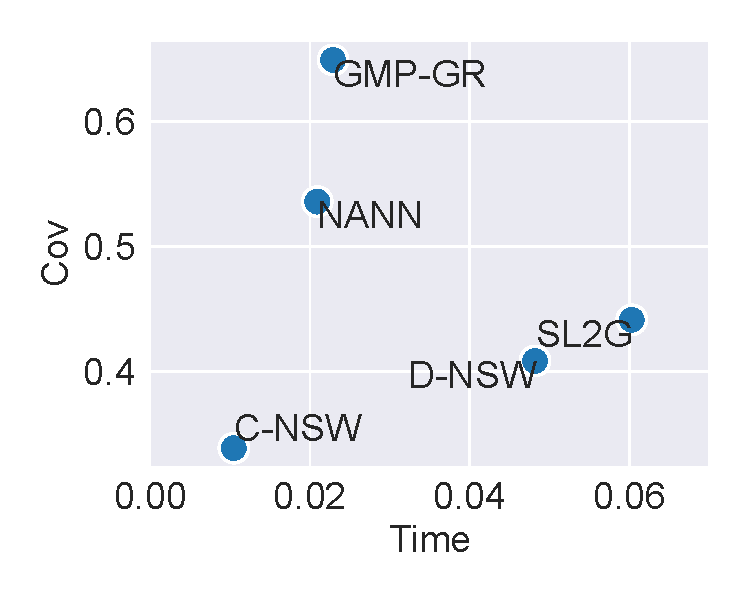
\includegraphics[width=0.47\linewidth]{figures/gmpgr/efficiency_Video.pdf}}
    \subfloat[MVideo]{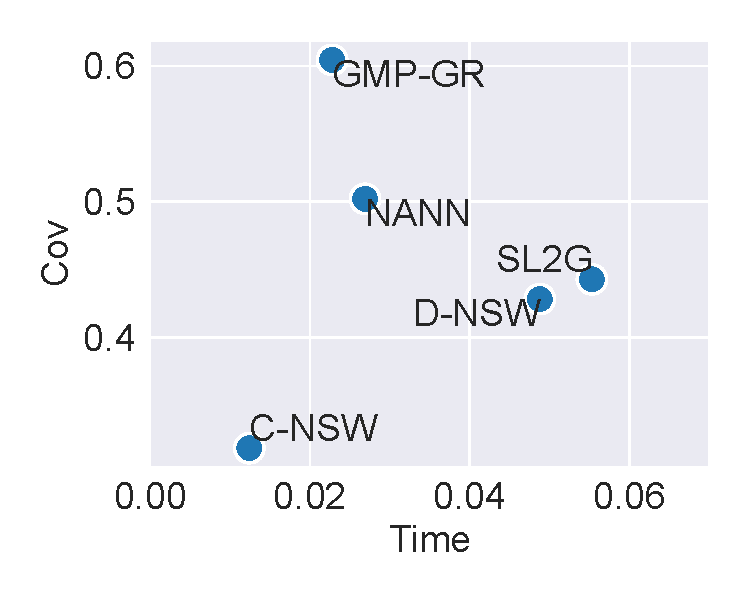
\includegraphics[width=0.48\linewidth]{figures/gmpgr/efficiency_MVideo.pdf}}
    \\[-0.5ex]
    \subfloat[Explore]{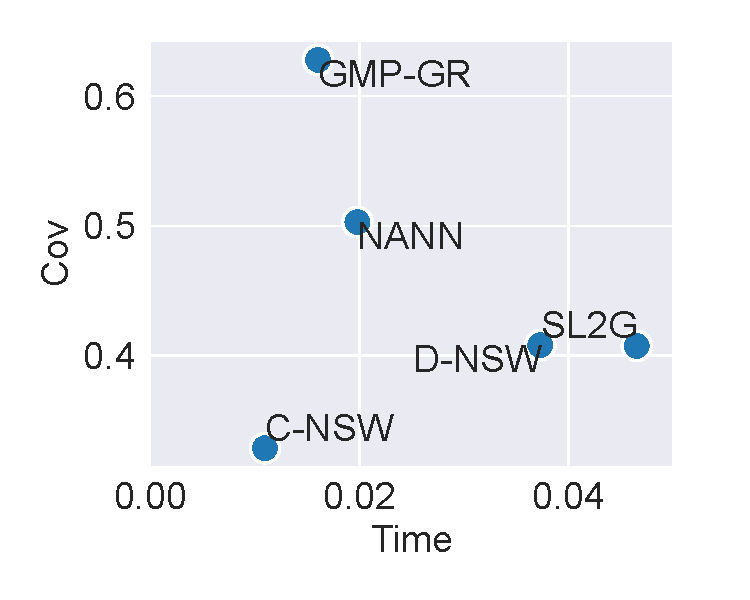
\includegraphics[width=0.47\linewidth]{figures/gmpgr/efficiency_Explore.pdf}}
    \subfloat[Fresh]{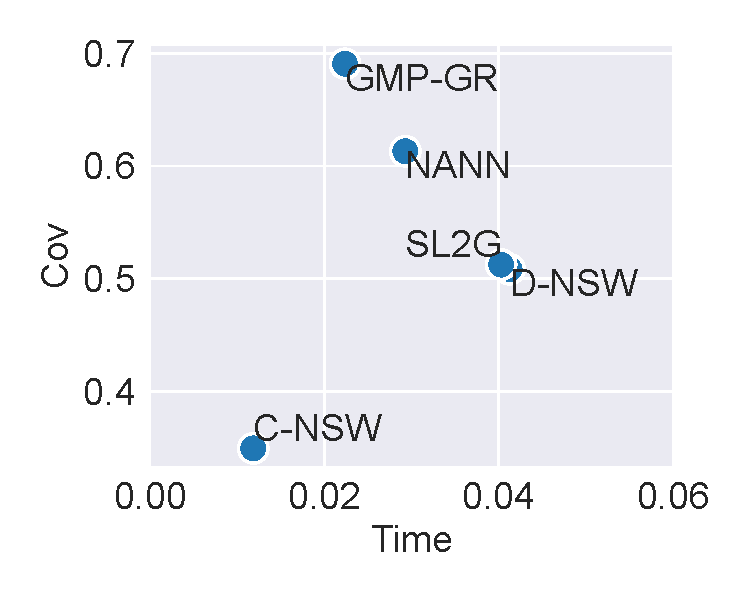
\includegraphics[width=0.47\linewidth]{figures/gmpgr/efficiency_Fresh.pdf}}
    \caption{Correlation between retrieval performance and efficiency on all four datasets. Methods closer to the upper-left corner achieve higher Cov with lower time cost.}
    \label{gmpgr:fig:efficiency}
\end{figure}

\paragraph{Ablation Study.}
We conduct an ablation study on GMP-GR in Figure~\ref{gmpgr:fig:ablation}, comparing it with two variants, \ie, GMP-GR-P and GMP-GR-M. The four panels jointly report Cov, retrieval speed, Rec@10, and Rec@100, allowing the effects on effectiveness and efficiency to be read together.
GMP-GR-P replaces MUIRML with a single supervision of the behavior in which a user visits an item, and GMP-GR-M substitutes HiPANNS with a standard HNSW search algorithm.
Specifically, we find that GMP-GR consistently outperforms both GMP-GR-P and GMP-GR-M across different datasets.
This superiority can be attributed to two key factors. First, MUIRML significantly enhances the relevance estimation accuracy and pathfinding efficiency. Second, HiPANNS prevents the graph-based ANNS process from succumbing to local optima by distributed and co-optimized search.
In addition, GMP-GR also shows a notable advantage in retrieval speed that replacing HiPANNS with a standard HNSW search algorithm can result in a great degradation of retrieval speed. This observation underscores the pivotal role of HiPANNS in acceleration. Furthermore, a more effective user-item relevance metric not only enhances the accuracy but also reduces traversal steps to converge to optimal candidates.

\begin{figure}[t]
    \centering
    \subfloat[Cov]{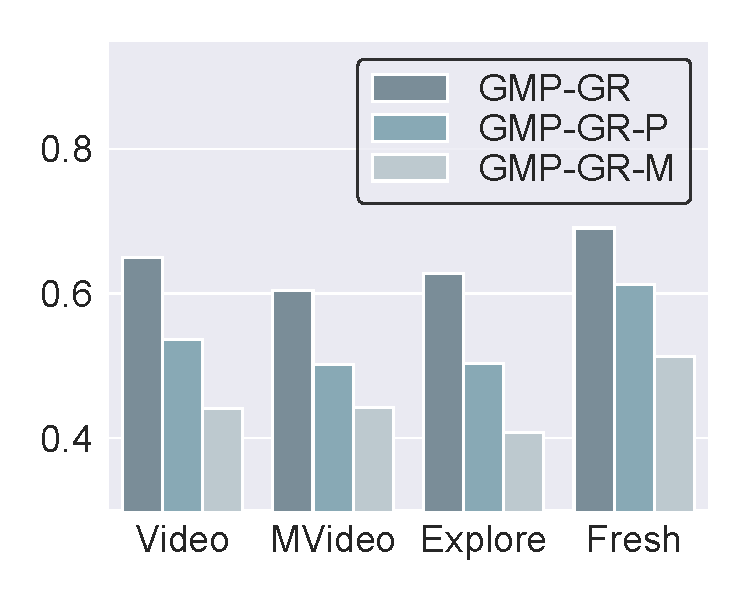
\includegraphics[width=0.42\linewidth]{figures/gmpgr/ablation_Cov.pdf}}
    \subfloat[Speed~($10^6$ items / sec)]{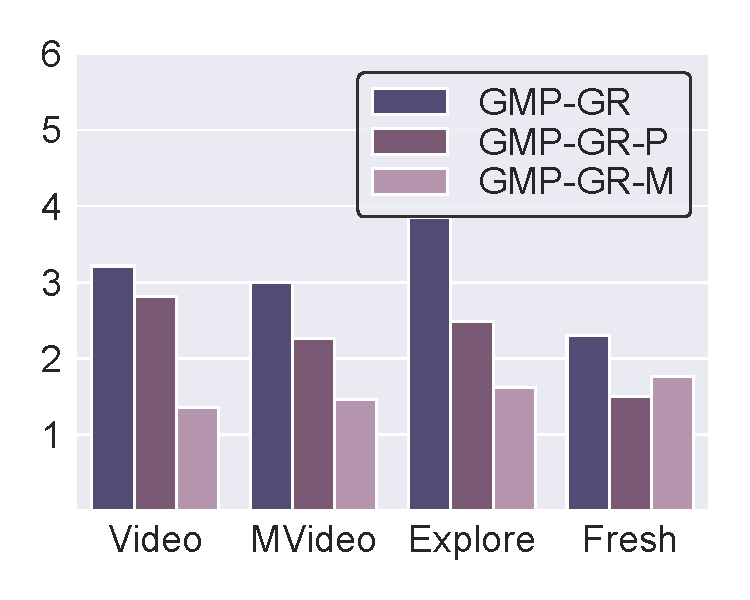
\includegraphics[width=0.42\linewidth]{figures/gmpgr/ablation_ItemPerS.pdf}}
    \\[-0.5ex]
    \subfloat[Rec@10]{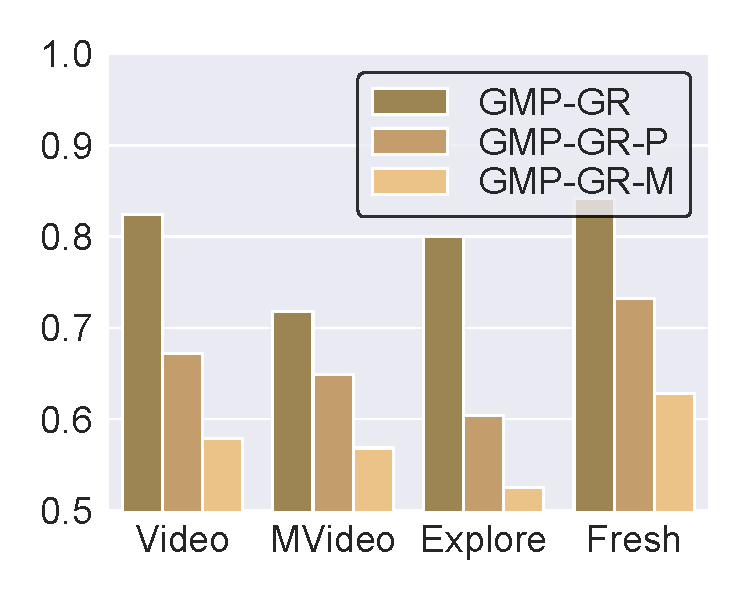
\includegraphics[width=0.42\linewidth]{figures/gmpgr/ablation_Rec10.pdf}}
    \subfloat[Rec@100]{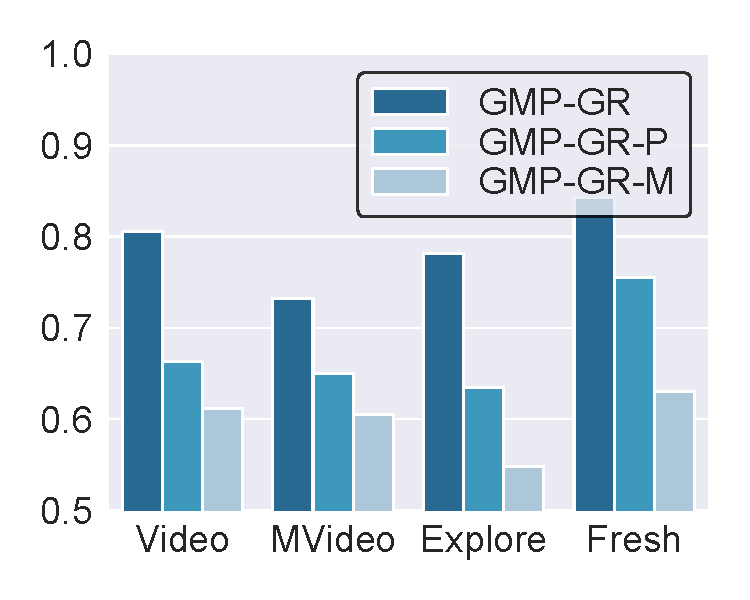
\includegraphics[width=0.42\linewidth]{figures/gmpgr/ablation_Rec100.pdf}}
    \caption{Ablation study of GMP-GR across retrieval effectiveness and efficiency metrics.}
    \label{gmpgr:fig:ablation}
\end{figure}

\FloatBarrier
\subsection{Online Testing}

We deploy GMP-GR in the Baidu Mobile APP for two services supported by five servers for online testing.
Service 1 is for the main recommendation list on the initial page.
Service 2 is for the next recommendation sequence that can be accessed after clicking on a video in immersive mode.

\subsubsection{Time on Page and Daily Active Users}

Table~\ref{gmpgr:tab:user_exp} depicts the impact of deploying GMP-GR on time on page and daily active users. Our results indicate a significant improvement in time on page and daily active users across the two services.
The integral components of GMP-GR, MUIRML, and HiPANNS, contribute to a $0.57\%$ and $0.23\%$ improvement in time on page, respectively.
Our findings suggest that the deployment of GMP-GR with improved modules has positively impacted user engagement and satisfaction.

\begin{table}[t]
    \caption{Online user statistics for two services.}
    \label{gmpgr:tab:user_exp}
    \centering
    \begin{tabular}{c|cc|cc}
        \toprule
        & \multicolumn{2}{c|}{Time on Page} & \multicolumn{2}{c}{Daily Active Users} \\
        & \textit{Service 1} & \textit{Service 2} & \textit{Service 1} & \textit{Service 2} \\
        \midrule
        GMP-GR & +1.13\% & +1.19\% & +0.23\% & +0.50\% \\
        \bottomrule
    \end{tabular}
\end{table}

\subsubsection{Query Throughput}
We also examine the query throughput influenced by the system acceleration strategies. The results demonstrate a strong improvement in query throughput, with an approximate doubling of throughput in the two services. Specifically, our analysis shows that the compilation optimization has led to a $74\%$ and $75\%$ increase in throughput by simplifying the computational graphs. Similarly, the model quantization has resulted in a $26\%$ and $25\%$ increase in throughput by decreasing DNN-based calculations. These findings underscore the effectiveness of GMP-GR in optimizing query processing and system efficiency.

\subsubsection{Statistical Analysis of Traffic and Latency}

\begin{figure}[t]
    \centering
    \subfloat[Traffic of two weeks in June, 2024.]{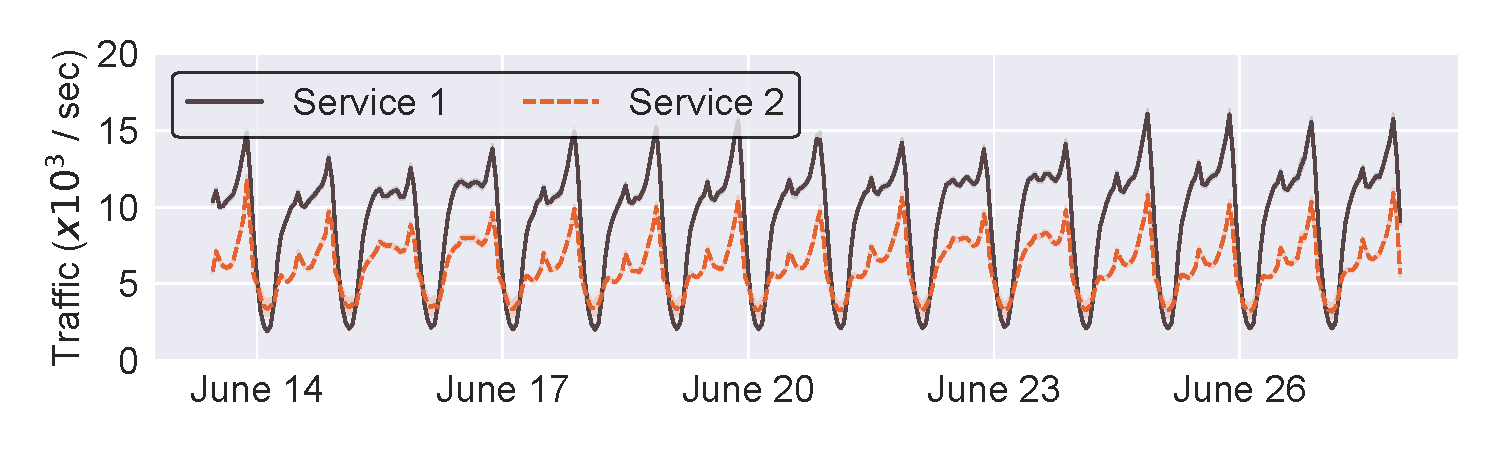
\includegraphics[width=\linewidth]{figures/gmpgr/timestamp_traffic.pdf}\label{gmpgr:fig:timestamp_traffic}}\\
    \subfloat[Latency in one day.]{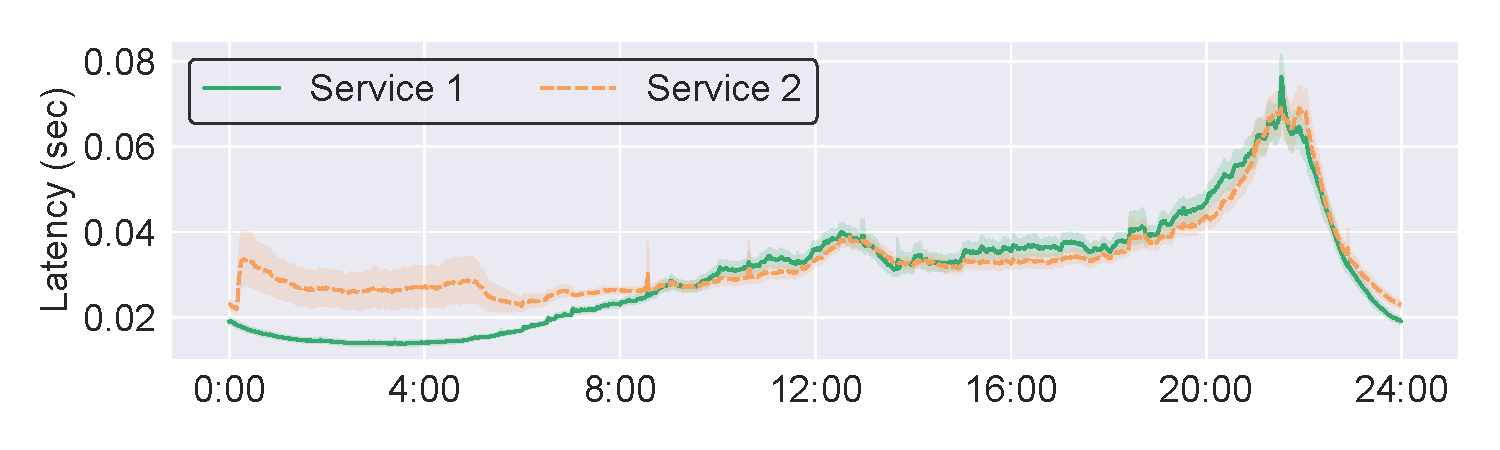
\includegraphics[width=\linewidth]{figures/gmpgr/timestamp_latency.pdf}\label{gmpgr:fig:timestamp_latency}}
    \caption{Temporal statistics of traffic and latency.}
    \label{gmpgr:fig:timestamp_traffic_latency}
\end{figure}

We collect traffic and latency statistics per second, which are recorded in a distributed manner at five servers in two services.
First, we examine the temporal patterns as shown in Figure~\ref{gmpgr:fig:timestamp_traffic_latency}. Specifically, Figure~\ref{gmpgr:fig:timestamp_traffic} illustrates the traffic trends over a two-week period, highlighting periodic fluctuations in query volumes. Meanwhile, Figure~\ref{gmpgr:fig:timestamp_latency} provides a more granular view of latency statistics over a 24-hour cycle, revealing variations in online response times in one day.
Moreover, we investigate the distributions of traffic and latency and explore their correlations in Figure~\ref{gmpgr:fig:service_traffic_latency}. The result indicates a direct relationship between query traffic and latency, with higher traffic volumes leading to longer response times. Furthermore, we observe distinct patterns in the latency-traffic relationships across five servers, reflecting divergence in computational resources and workload distribution.
Finally, Figures~\ref{gmpgr:fig:server_traffic} and~\ref{gmpgr:fig:server_latency} summarize the traffic and latency statistics across five servers, providing insights into the performance characteristics in terms of query processing and response times.

Taken together, the offline and online results show that search scaling cannot be reduced to faster graph traversal alone. Retrieval quality, navigation behavior, and GPU execution efficiency must be optimized jointly for the learned relevance signal to remain effective under production-scale traffic. This system-level evidence completes the progression from semantic representation through observational efficiency to large-scale search developed across the three technical chapters.

\begin{figure}[t]
    \centering
    \subfloat[Service 1]{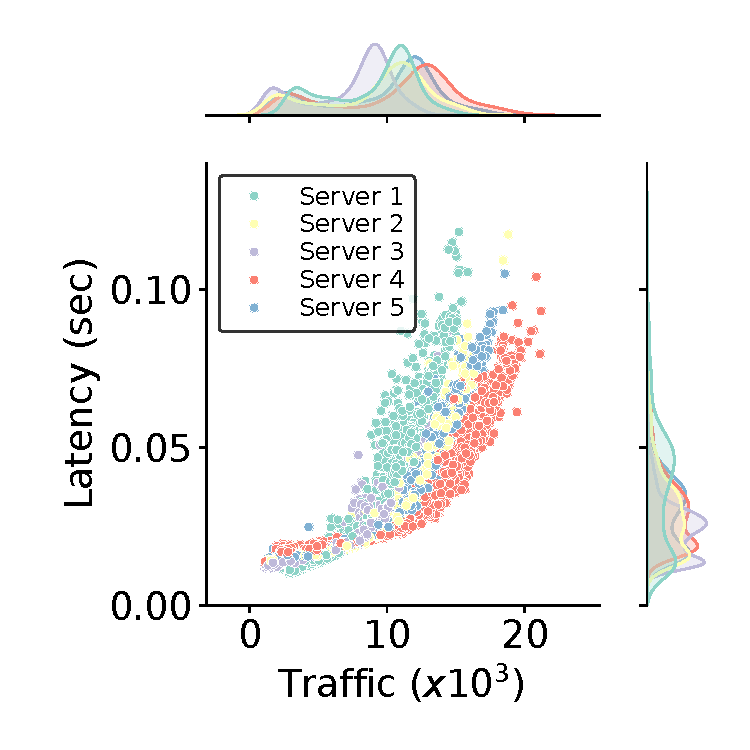
\includegraphics[width=0.38\linewidth]{figures/gmpgr/service_1_traffic_latency.pdf}}
    \hspace{0.04\linewidth}
    \subfloat[Service 2]{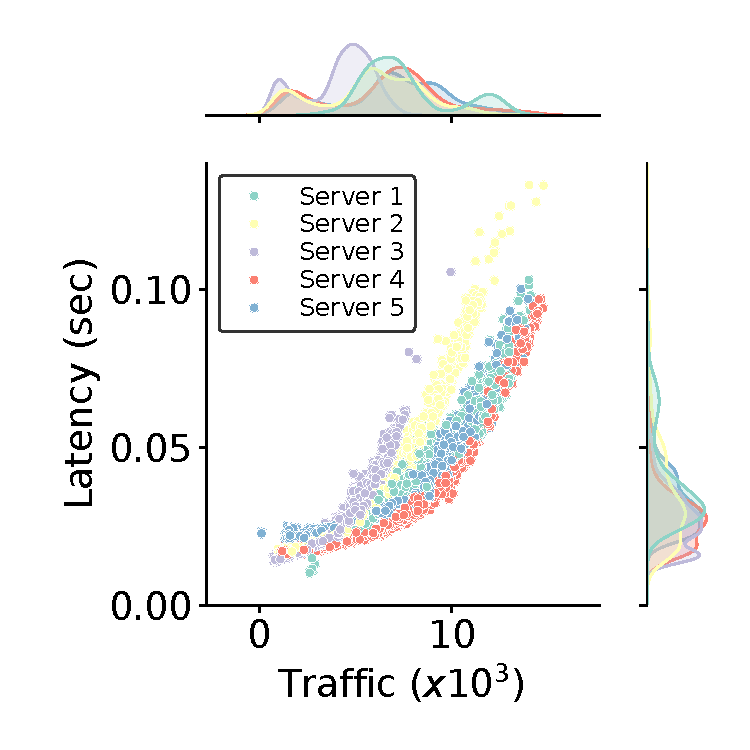
\includegraphics[width=0.38\linewidth]{figures/gmpgr/service_2_traffic_latency.pdf}}\\[-0.5ex]
    \subfloat[Traffic across servers]{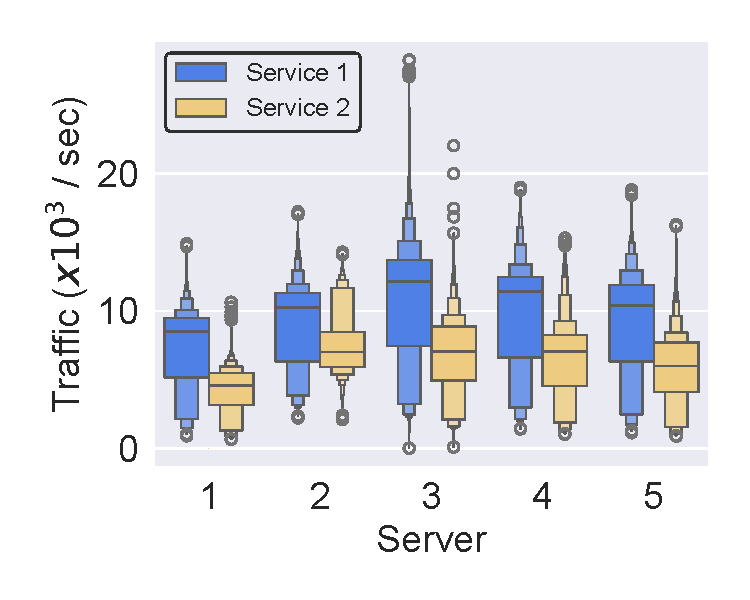
\includegraphics[width=0.38\linewidth]{figures/gmpgr/server_traffic.pdf}\label{gmpgr:fig:server_traffic}}
    \hspace{0.04\linewidth}
    \subfloat[Latency across servers]{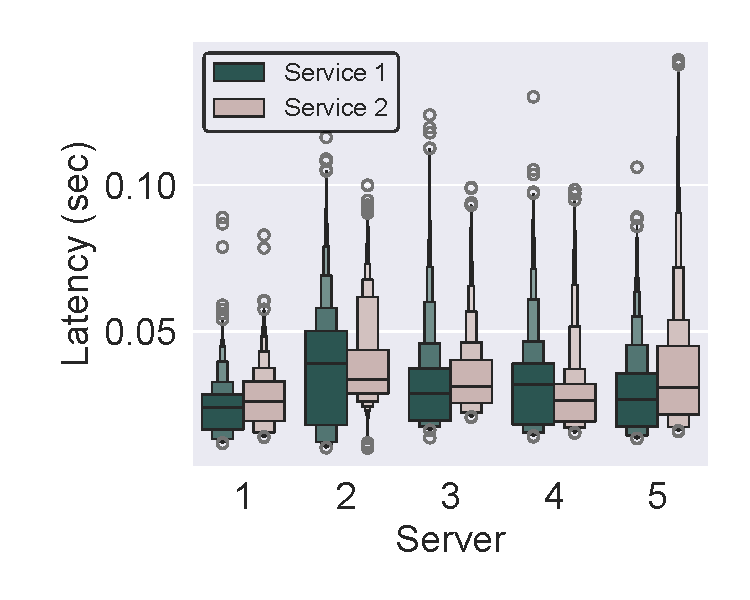
\includegraphics[width=0.38\linewidth]{figures/gmpgr/server_latency.pdf}\label{gmpgr:fig:server_latency}}
    \caption{Distributions and relationships of traffic and latency across two services and five servers.}
    \label{gmpgr:fig:service_traffic_latency}
\end{figure}

\FloatBarrier
\section{Chapter Summary}

This chapter addressed the search-scaling stage of the thesis by studying how a learned relevance signal can be used for accurate and efficient retrieval over web-scale recommendation collections. It introduced GMP-GR, which combines multi-relational user-item relevance metric learning with hierarchically parallel graph search and system-level GPU optimizations. Offline experiments showed consistent gains in retrieval quality and a favorable balance between accuracy and search speed. The ablation results attributed these gains to both MUIRML and HiPANNS. Online deployment further demonstrated improvements in user engagement and query throughput under production traffic.

Within the thesis, this chapter completes the progression from representation to deployment. Chapter~\ref{ch:universal-video-retrieval} established semantic generalization across retrieval tasks and domains, while Chapter~\ref{ch:spatiotemporal-scaling} studied how observational density affects the evidence preserved by video embeddings. The present chapter showed that these representations must also be paired with a relevance metric, graph-navigation strategy, and execution system that remain effective at large candidate scale. Together, the three studies position scalable video retrieval as a joint problem of semantic coverage, observational efficiency, and search-system efficiency.

\chapter{Conclusions and Future Directions}
\label{ch:conclusion}

\section{Conclusions}
\label{sec:conclusions}

Modern video retrieval must operate across heterogeneous query forms, long and informationally dense videos, and candidate collections whose scale precludes exhaustive scoring. This thesis has argued that these demands are best understood as three sequential scaling challenges along the retrieval pipeline: semantic scaling, observational scaling, and search scaling. Each challenge corresponds to a distinct stage of the pipeline, and each presents a distinct bottleneck that is not eliminated by optimizing an upstream stage alone.

This thesis is organized around three studies, each addressing one of these stages. The first study establishes the representation foundation through semantic scaling. The second extends the investigation to observational scaling, studying how visual evidence should be allocated for long and multi-granular video retrieval. The third addresses search scaling, examining the retrieval infrastructure required when learned relevance signals are deployed at web scale. Together, they support a shared thesis: scalable video retrieval requires structure-aware scaling across semantic capability, visual observation, and search execution, and such scaling should be evaluated through generalization beyond the conditions under which each stage is optimized. The key findings and contributions of each study are summarized below.

\subsection{Summary of Contributions}

\paragraph{Chapter~\ref{ch:universal-video-retrieval}: Universal Video Retrieval through Capability-Oriented Learning.}
Existing video retrieval research often evaluates on a narrow set of benchmarks, leaving critical capability gaps unexamined. This work proposed the General Video Embedder (GVE) framework, which (1) identified deficiencies in fine-grained, temporal, and partially relevant retrieval through a structured assessment across 16 public datasets; (2) introduced V-SynFlow, a synthesis pipeline that produced the Universal Video Retrieval Dataset (UVRD) with over 1.55 million multi-task video-text pairs targeting those gaps; and (3) developed a Modality Pyramid curriculum that leverages inherent task hierarchies for progressive learning. The resulting GVE model achieved state-of-the-art zero-shot performance across diverse retrieval scenarios, demonstrating that conventional benchmarks poorly correlate with holistic retrieval capability and that partially relevant retrieval is a pivotal yet overlooked real-world challenge.

\paragraph{Chapter~\ref{ch:spatiotemporal-scaling}: Spatiotemporal Scaling Analysis and Efficient Inference.}
The way videos are observed during embedding generation fundamentally affects retrieval quality, yet this dimension has received limited attention. This work introduced the Multi-Granular Long Video Retrieval (MG-LVR) benchmark, the first benchmark supporting multi-granular queries for long-form video retrieval. Evaluation across 23 multimodal embedding models revealed a significant granularity gap---fine-grained retrieval lags coarse-grained performance by over 75\% under sparse sampling. The comprehensive spatiotemporal scaling analysis identified actionable principles including frame-count anchoring and granularity-dependent token allocation. Building on these insights, the Video Embedding Waterfall (VEterfall) framework was proposed, achieving up to 20\% improvement in fine-grained query performance while operating in 4$\times$ to 16$\times$ more efficient inference settings.

\paragraph{Chapter~\ref{ch:scale-efficient-retrieval}: Scale-Efficient Retrieval via Co-Designed Metrics, Graph Search, and GPU Execution.}
A learned retrieval signal must not only be accurate but also searchable and deployable at scale. This work proposed the GPU-accelerated Multi-relational Parallel Graph Retrieval (GMP-GR) framework with three key innovations: (1) Multi-relational User-Item Relevance Metric Learning (MUIRML) that unifies diverse user behaviors through multi-objective optimization and employs a self-covariant loss to enhance graph pathfinding; (2) Hierarchically Parallel Approximate Nearest Neighbor Search (HiPANNS) that conducts breadth-depth-balanced graph traversal with adaptive GPU aggregation for irregular neural computation; and (3) system-level optimizations including traffic dispersal, compilation optimization, model quantization, and timely stream update. Deployed across more than twenty applications at Baidu, GMP-GR serves hundreds of millions of users with throughput exceeding one hundred million requests per second, improving more than 3\% time of page for users.

\subsection{Unified Methodology and Insights}

Together, these studies form a coherent methodology that extends from representation learning through observation-aware embedding generation to deployment-scale retrieval. Each study addresses the scaling bottleneck at its respective stage of the pipeline, and each depends on the conclusions of the preceding one: the first study establishes what capabilities a retrieval model should possess, the second examines how visual observation affects the realization of those capabilities, and the third ensures that the resulting retrieval signals can scale to large candidate collections.

A central insight shared across all three studies is that scaling capacity does not automatically translate into retrieval generalization. Scaling model size alone does not cover the full breadth of semantic capabilities. Increasing observation density does not automatically improve fine-grained retrieval. Improving metric accuracy does not guarantee faster search. Within the scope of this thesis, generalizability serves as an empirical criterion for assessing whether scaling has been performed in a structure-aware manner at each stage of the retrieval pipeline: only by understanding the structure of the bottleneck and designing accordingly does the system remain effective under conditions it was not explicitly optimized for. This unified view provides practical guidance for building video retrieval systems that support richer semantic tasks, adapt to different sampling budgets, and scale to large candidate spaces while maintaining effectiveness across heterogeneous queries, videos, and deployment conditions.

The notion of generalizability evolves across the three stages of the retrieval pipeline. In semantic scaling, it concerns whether the learned representation transfers across query modalities, retrieval domains, and relevance granularities. In observational scaling, it concerns whether retrieval quality remains robust when visual evidence is resampled across different densities, durations, and query granularities. In search scaling, it concerns whether the learned retrieval signal remains effective under different deployment contexts, traffic patterns, and serving constraints. These forms are not identical, but they are unified by the same principle: scaling is meaningful only when the resulting capability transfers beyond the narrow condition under which it is optimized.

\section{Future Directions}
\label{sec:future-works}

The three studies in this thesis address distinct dimensions of video retrieval, yet each opens avenues that extend beyond the scope of the present work. This section outlines four directions for future research, organized from immediate extensions of the current findings to longer-term visions for the field.

\subsection{Query- and Content-Adaptive Observation}

The results in this thesis suggest that different queries do not require the same visual evidence. Coarse topical queries, fine-grained event queries, visual queries, and composed queries may prefer different allocations of temporal coverage and spatial detail. A natural next step is to make the observation policy adaptive to both the query and the video content, so that the system can spend computation where evidence is most likely to matter.

One promising direction is to develop lightweight query classifiers that predict the optimal sampling configuration before video encoding. Such classifiers could analyze query text to estimate temporal granularity, spatial specificity, and relevance distribution patterns, then select appropriate frame counts and resolutions accordingly. Another direction is content-aware sampling, where the system analyzes video content to identify information-dense segments that warrant higher sampling density. This could involve preliminary passes with cheap feature extractors to detect scene changes, action boundaries, or semantically rich regions, followed by targeted dense sampling in those regions.

More ambitiously, end-to-end differentiable sampling policies could be trained jointly with the retrieval model, allowing the system to learn task-specific observation strategies through reinforcement learning or attention mechanisms. Such approaches could enable dynamic allocation of computational resources within a single video, concentrating frames on moments most relevant to the query while maintaining sufficient coverage to avoid missing distributed evidence.

\subsection{Retrieval-Oriented Video Foundation Models}

Current multimodal models are often trained for broad vision-language instruction following or contrastive alignment. Future video foundation models could be trained more explicitly around retrieval requirements, including partial relevance, temporal evidence preservation, multimodal query support, robustness under sparse observation, and compatibility with efficient search.

The findings from Chapter~\ref{ch:spatiotemporal-scaling} suggest that current video models exhibit frame-count anchoring, where temporal representations become overly specialized to specific training densities. Future training objectives could explicitly encourage density-invariant representations, perhaps through multi-density contrastive learning where the same video must retrieve the same query across different sampling configurations. Similarly, the capability gaps identified in Chapter~\ref{ch:universal-video-retrieval} suggest that training data should more systematically cover fine-grained temporal reasoning, spatial relation understanding, and composed query scenarios.

Another important direction is developing video foundation models that natively support partial relevance, where a video is relevant to a query even if only a portion of its content matches. This requires moving beyond global video-level representations toward segment-aware or moment-aware embeddings that can capture localized relevance. Such models might employ hierarchical encoding schemes that maintain both coarse global summaries and fine-grained local representations, enabling retrieval at multiple granularity levels simultaneously.

Furthermore, future video foundation models should be designed with deployment constraints in mind. This includes compatibility with approximate search structures, efficient update mechanisms for dynamic corpora, and representations that remain discriminative even under aggressive compression or quantization for large-scale storage.

\subsection{Joint Optimization of Embeddings and Indexes}

Large-scale retrieval depends on both representation quality and index searchability. Future work can further close the loop between embedding learning and index behavior, optimizing models not only for pairwise similarity or ranking accuracy, but also for graph navigability, update efficiency, memory footprint, batching behavior, and hardware execution.

The work in Chapter~\ref{ch:scale-efficient-retrieval} demonstrated that metric properties like approximate triangle inequality significantly impact graph traversal efficiency. Future research could explore learned metrics that are explicitly optimized for specific index structures, such as hierarchical navigable small world graphs or product quantization schemes. This could involve differentiable approximations of graph traversal that allow gradient-based optimization of embedding spaces for both retrieval accuracy and search efficiency.

Another promising direction is co-designing embeddings and indexes for dynamic scenarios where the candidate corpus evolves over time. This requires representations that support efficient incremental indexing without full rebuilds, as well as metrics that remain stable as the corpus distribution shifts. Online learning approaches that continuously update both embeddings and index structures could enable more responsive retrieval systems for applications like news recommendation or trending content discovery.

Hardware-aware embedding learning represents another frontier. Different hardware platforms (CPUs, GPUs, TPUs, specialized accelerators) have distinct computational characteristics that affect retrieval performance. Future work could develop embedding models that are co-optimized with specific hardware constraints, such as memory bandwidth, parallelism patterns, or instruction set capabilities. This could lead to significant efficiency gains in large-scale deployment scenarios.

\subsection{Evaluation Protocols for Real-World Video Retrieval}

Existing benchmarks remain useful, but real retrieval systems involve changing corpora, mixed query modalities, variable video duration, latency budgets, freshness constraints, and downstream ranking interactions. Building evaluation protocols that reflect these conditions will be essential for measuring progress beyond static benchmark recall.

The benchmarks developed in this thesis, including UVRD and MG-LVR, provide foundations for more comprehensive evaluation, but significant gaps remain. Future evaluation frameworks should incorporate temporal dynamics, where videos are added, removed, or modified over time, testing the system's ability to maintain retrieval quality in evolving corpora. They should also include diverse query modalities within the same evaluation, requiring systems to handle text, image, video, and composed queries seamlessly.

Latency and throughput constraints should be explicitly incorporated into evaluation metrics, moving beyond pure recall measurements to efficiency-adjusted metrics that reward systems achieving high accuracy within computational budgets. This is particularly important for real-time applications where response time directly impacts user experience.

Downstream task evaluation represents another important direction. Rather than evaluating retrieval in isolation, future protocols should measure how retrieval quality affects downstream tasks like recommendation, content discovery, or user engagement. This requires end-to-end evaluation frameworks that integrate retrieval with ranking, filtering, and presentation components.

Finally, evaluation should consider fairness, diversity, and serendipity aspects of retrieval, ensuring that systems do not merely optimize for narrow relevance metrics but also support broader information access goals. This includes evaluating retrieval across different user populations, content categories, and temporal contexts to ensure robust and equitable performance.


% ============================================================
% APPENDIX
% ============================================================

\clearpage
\appendix
\chapter{Full Publication List}
\label{ch:publications}

This appendix provides the complete list of publications by the author during his Ph.D. study. The first three first-authored publications form the basis of the three main research chapters of this dissertation, addressing the semantic, observational, and search scaling challenges of video retrieval, respectively. The remaining first-authored publications cover related but independent work in federated graph learning and labor market modeling. The co-authored publications reflect collaborative contributions in multimodal retrieval and human mobility modeling.

\section*{Publications Involved in This Thesis}

\begin{enumerate}
    \item \textbf{Chapter~\ref{ch:universal-video-retrieval} (ACM MM 2026).} Zhuoning Guo, Mingxin Li, Yanzhao Zhang, Dingkun Long, Pengjun Xie, and Xiaowen Chu. ``Towards Universal Video Retrieval: Generalizing Video Embedding via Synthesized Multimodal Pyramid Curriculum.'' Accepted for publication in \emph{Proceedings of the 34th ACM International Conference on Multimedia (MM '26)}. ACM, 2026.

    \item \textbf{Chapter~\ref{ch:spatiotemporal-scaling} (AAAI 2027, submitted).} Zhuoning Guo, Tingyu Song, Mingxin Li, Yanzhao Zhang, Dingkun Long, Pengjun Xie, and Xiaowen Chu. ``Demystifying Spatiotemporal Scaling Laws of Multimodal Video Embeddings.'' Submitted to the \emph{Forty-First AAAI Conference on Artificial Intelligence (AAAI-27)}, 2027.

    \item \textbf{Chapter~\ref{ch:scale-efficient-retrieval} (WebConf 2026).} Zhuoning Guo, Guangxing Chen, Qian Gao, Xiaochao Liao, Jianjia Zheng, Lu Shen, and Hao Liu. ``GPU-accelerated Multi-relational Parallel Graph Retrieval for Web-scale Recommendations.'' In \emph{Proceedings of the ACM Web Conference 2026 (WWW '26)}. ACM, 2026.
\end{enumerate}

\section*{Other First-Author Publications}

\begin{enumerate}
    \item \textbf{[ECML-PKDD 2026]} Zhuoning Guo, Ruiqian Han, and Hao Liu. ``Against Multifaceted Graph Heterogeneity via Asymmetric Federated Prompt Learning.'' In \emph{Proceedings of the European Conference on Machine Learning and Principles and Practice of Knowledge Discovery in Databases (ECML-PKDD '26)}, 2026.

    \item \textbf{[PAKDD 2025, Oral]} Zhuoning Guo, Le Zhang, Hengshu Zhu, Weijia Zhang, Hui Xiong, and Hao Liu. ``Labor Migration Modeling through Large-scale Job Query Data.'' In \emph{Advances in Knowledge Discovery and Data Mining: Pacific-Asia Conference on Knowledge Discovery and Data Mining (PAKDD '25)}, 2025.

    \item \textbf{[KDD 2024, Oral]} Zhuoning Guo, Duanyi Yao, Qiang Yang, and Hao Liu. ``HiFGL: A Hierarchical Framework for Cross-silo Cross-device Federated Graph Learning.'' In \emph{Proceedings of the 30th ACM SIGKDD Conference on Knowledge Discovery and Data Mining (KDD '24)}. ACM, 2024.

    \item \textbf{[KDD 2024 Workshop]} Zhuoning Guo, Le Zhang, Hengshu Zhu, Weijia Zhang, Hui Xiong, and Hao Liu. ``Discrepant Homophily Co-Preserved Graph Convolutional Network for Labor Migration Forecasting.'' In \emph{Workshop of Talent Management Computing (TMC) at SIGKDD 2024}, 2024.

    \item \textbf{[KDD 2022, Oral]} Zhuoning Guo, Hao Liu, Le Zhang, Qi Zhang, Hengshu Zhu, and Hui Xiong. ``Talent Demand-Supply Joint Prediction with Dynamic Heterogeneous Graph Enhanced Meta-Learning.'' In \emph{Proceedings of the 28th ACM SIGKDD Conference on Knowledge Discovery and Data Mining (KDD '22)}. ACM, 2022.

    \item \textbf{[arXiv]} Zhuoning Guo, Hao Liu, Le Zhang, Qi Zhang, Hengshu Zhu, and Hui Xiong. ``Convergence-aware Clustered Federated Graph Learning Framework for Collaborative Inter-company Labor Market Forecasting.'' arXiv preprint, 2024.
\end{enumerate}

\section*{Co-Authored Publications}

\begin{enumerate}
    \item \textbf{[ICML 2026]} Qiuchen Wang, Shihang Wang, Yu Zeng, Qiang Zhang, Fanrui Zhang, Zhuoning Guo, Bosi Zhang, Wenxuan Huang, Lin Chen, Zehui Chen, Pengjun Xie, and Ruixue Ding. ``VimRAG: Navigating Massive Visual Context in Retrieval-Augmented Generation via Multimodal Memory Graph.'' In \emph{Proceedings of the 43rd International Conference on Machine Learning (ICML '26)}, 2026.

    \item \textbf{[ACL 2026]} Tingyu Song, Yanzhao Zhang, Mingxin Li, Zhuoning Guo, Dingkun Long, Pengjun Xie, Siyue Zhang, Yilun Zhao, and Shu Wu. ``Rethinking Composed Image Retrieval Evaluation: A Fine-Grained Benchmark from Image Editing.'' In \emph{Proceedings of the 64th Annual Meeting of the Association for Computational Linguistics (ACL '26)}, 2026.

    \item \textbf{[AAAI 2024, Oral]} Wen Shuo Chao, Zhaopeng Qiu, Likang Wu, Zhuoning Guo, Zhi Zheng, Hengshu Zhu, and Hao Liu. ``A Cross-View Hierarchical Graph Learning Hypernetwork for Skill Demand-Supply Joint Prediction.'' In \emph{Proceedings of the Thirty-Eighth AAAI Conference on Artificial Intelligence (AAAI '24)}, 2024.

    \item \textbf{[AAAI 2023]} Yang Liu, Yu Rong, Zhuoning Guo, Nuo Chen, Tingyang Xu, Fugee Tsung, and Jia Li. ``Human Mobility Modeling During the COVID-19 Pandemic via Deep Graph Diffusion Infomax.'' In \emph{Proceedings of the Thirty-Seventh AAAI Conference on Artificial Intelligence (AAAI '23)}, 2023.

    \item \textbf{[TVCG]} Wenyuan Kong, Zhaoyun Jiang, Shizhao Sun, Zhuoning Guo, Weiwei Cui, Ting Liu, Jian-Guang Lou, and Dongmei Zhang. ``Aesthetics++: Refining Graphic Designs by Exploring Design Principles and Human Preference.'' \emph{IEEE Transactions on Visualization and Computer Graphics}, 2022.
\end{enumerate}


% ============================================================
% BIBLIOGRAPHY
% ============================================================

\clearpage
\addcontentsline{toc}{chapter}{Bibliography}
\bibliographystyle{IEEEtran}
\bibliography{references/references}

\end{document}
